% The manuscript; cardiac-rings.pdf beside it is this file built with pdflatex, run three times
% (sh tools/paper-build.sh cardiac-rings). Paths such as code/fourier/existence.py and data/fourier-stability-N8.json
% are relative to the paper's folder (the folder that holds paper/, code/ and data/). The figures in figures/ are drawn
% by code/plot_cardiac_rings.py from stored files.
\documentclass[11pt]{article}
\usepackage[letterpaper,margin=1in]{geometry}
\usepackage[T1]{fontenc}
\usepackage{lmodern}
\usepackage{amsmath,amssymb,amsthm}
\usepackage{array}
\usepackage{booktabs}
\usepackage{graphicx}
\usepackage{microtype}
\setlength{\emergencystretch}{2em}
\usepackage{xurl}
\usepackage[hidelinks]{hyperref}

\hypersetup{
  pdftitle={Stable Rotating Waves in Rings of a Modified Ventricular Cell Model: Computer-Assisted Proofs},
  pdfauthor={Chase Hendrick}}

\newtheorem{theorem}{Theorem}
\renewcommand{\thetheorem}{\Alph{theorem}}
\newtheorem{lemma}{Lemma}[section]
\newtheorem{proposition}[lemma]{Proposition}
\newtheorem{thmx}[lemma]{Theorem}
\newtheorem{corollary}[lemma]{Corollary}
\theoremstyle{definition}
\newtheorem{definition}[lemma]{Definition}
\newtheorem{remark}[lemma]{Remark}

\newcommand{\R}{\mathbb{R}}
\newcommand{\C}{\mathbb{C}}
\newcommand{\Z}{\mathbb{Z}}
\newcommand{\re}{\operatorname{Re}}
\newcommand{\im}{\operatorname{Im}}
\newcommand{\spec}{\operatorname{spec}}
\newcommand{\Ran}{\operatorname{Ran}}
\newcommand{\rank}{\operatorname{rank}}
\newcommand{\one}{\mathbf{1}}
\newcommand{\Dsp}{\mathcal{D}}
\newcommand{\Xsp}{\mathcal{X}}
\newcommand{\Lop}{\mathcal{L}}
\DeclareUrlCommand\file{\urlstyle{tt}}

\title{\Large\bfseries Stable Rotating Waves in Rings of a Modified Ventricular Cell Model:\\ Computer-Assisted Proofs}
\author{Chase Hendrick\\[0.2em] {\small Independent Researcher}\\ {\small\href{mailto:chase@hendrickresearch.com}{\texttt{chase@hendrickresearch.com}}}\\ {\small ORCID \href{https://orcid.org/0009-0002-9754-6087}{0009-0002-9754-6087}}}
\date{}

\begin{document}
\maketitle

\begin{abstract}
We give computer-assisted proofs for Erhardt's 18-state modification of the ten Tusscher--Panfilov 2006 endocardial ventricular cell model at slow delayed rectifier conductance $G_{Ks} = 0.0275$~nS/pF, 1.46 per cent below the first supercritical Hopf point he computed numerically. Rings of $N$ identical cells, coupled diffusively through the voltage with strength $N^2/64000$ per ms, discretize the cable $u_t = f(u) + D\,u_{xx}$, $D = 1/64000$ per ms, on a ring of length 1. Rotating waves there are expected from equivariant Hopf theory; we prove them at explicit parameters.

For one cell, two proofs (CAPD and Arb, sharing only GMP and MPFR) give an orbitally asymptotically stable periodic orbit, with 17 nontrivial Floquet multipliers below $0.998642$ and $0.997859$ respectively, and an exact rational check shows both enclose the same orbit. For $N = 8, 16, 32, 64$ a rotating 1-wave exists, is locally unique and not synchronous, has minimal period $T = 2\pi/\omega$ enclosed to within $2 \times 10^{-25}$~ms, and is locally exponentially orbitally stable: the multiplier $1$ is algebraically simple and the other $18N - 1$ have modulus below $e^{-\delta T} < 0.9997321$, $\delta = 5 \times 10^{-6}$ per ms. A locally unique rotating 1-wave also exists for every $N \ge 8$, and a traveling wave for the cable, the limit of the ring waves.

Existence is a radii-polynomial argument in a weighted $\ell^1$ space, made uniform over $\varepsilon \in [0, 1/64]$ ($1/N^2$ for the rings, $0$ for the cable) in 73 pieces glued by ball inclusion. Stability rests on one Hill operator whose spectrum gives every Floquet multiplier with its algebraic multiplicity; a Riesz-projection homotopy shows it meets $\{\re\mu \ge -\delta\}$ only in the eigenvalues $i\omega N\Z$, each algebraically simple. For the single cell, a connected conductance family reaches a certified supercritical Hopf endpoint. Its 712-piece lower interval has uniform nontrivial multiplier bound $0.998413816$; a 68-piece amplitude family supplies the bridge. Quantitative uniform stability is proved only on the lower interval. Nothing is claimed for tissue.

\medskip
\noindent\textbf{Keywords:} cardiac cell model; modified ten Tusscher--Panfilov model; ring of coupled oscillators; rotating wave; Floquet multipliers; Hill operator; computer-assisted proof; ball arithmetic; radii polynomial.\\
\textbf{MSC 2020:} 37C27, 34C25, 92C30, 37M20, 65G20.
\end{abstract}

\section{Introduction}\label{sec:intro}

Detailed ionic models of cardiac cells are systems of a few dozen nonlinear ordinary differential equations whose right-hand sides contain exponentials, logarithms (Nernst potentials) and square roots. Their bifurcations are studied by numerical continuation. Erhardt and Solem analyzed reduced versions of the ten Tusscher--Panfilov 2006 (TP06) model \cite{tp2006} in this way \cite{es2021,es2022}, K\"ugler and coauthors related early afterdepolarizations to period doubling cascades and to folded nodes \cite{keb2017,keb2018}, and Erhardt \cite{erhardt2025} studied an 18-dimensional modification of the TP06 endocardial cell with reduced repolarization reserve, continued in the slow delayed rectifier conductance $G_{Ks}$. For that model he reports a supercritical Hopf bifurcation at $G_{Ks} = 0.027907858929580$~nS/pF with stable bifurcating cycles \cite[Table~2]{erhardt2025}.

This paper gives computer-assisted proofs for that model at $G_{Ks} = 0.0275$, about $1.46$ per cent below the Hopf value, for the single cell and for rings of $N$ identical cells coupled diffusively through the membrane potential. The ring is the simplest spatial object built from these cells: a periodic chain $x_0, \dots, x_{N-1}$ with
\begin{equation}\label{eq:ring}
  \dot x_j = f(x_j) + c\, E\,(x_{j-1} - 2x_j + x_{j+1}), \qquad j \in \Z_N, \qquad c = \frac{N^2}{64000}\ \text{per ms},
\end{equation}
where $f$ is the cell's vector field and $E$ the projection on the voltage. The coupling $c = N^2 D$ with $D = 1/64000$ is that of a ring of unit length discretized into $N$ cells. The ring is equivariant under the cyclic shift, and a rotating wave (a discrete traveling wave) is a solution $x_j(t) = \phi(\omega t + 2\pi j/N)$ with $\phi$ $2\pi$-periodic. That such waves exist near a Hopf point of a ring of identical cells is the generic expectation of $\Z_N$-equivariant Hopf theory \cite{gs1985}, \cite[Ch.~XVIII, Sect.~4]{gss1988}; we make no claim that their existence is surprising. What we add is a proof, at an explicit parameter value and explicit coupling strengths, of existence, local uniqueness, the minimal period and local exponential orbital stability, for the full 18-dimensional nonlinear cells.

\paragraph{Results.} Theorem~\ref{thm:cell} concerns the single cell. It has two parts, proved independently: one in the time domain with CAPD \cite{capd2021}, by a contraction argument for the Poincar\'e map, and one in Fourier space with Arb \cite{johansson2017}, by the method of this paper with $N = 1$. The two proofs use different interval arithmetic (CAPD with filib double intervals, and MPFR intervals for one center image; Arb ball arithmetic in FLINT), different translations of the model and different methods; they have in common only the multiprecision libraries GMP and MPFR, linked in separate builds. An exact rational check (Lemma~\ref{lem:link}) shows that they enclose the same orbit. We call the existence proof in Fourier space Stage~E (Section~\ref{sec:existence}) and the stability proof Stage~S (Section~\ref{sec:stability}), as the programs and their records do. Theorem~\ref{thm:ring} concerns the rings with $N = 8, 16, 32, 64$. Its existence part (Section~\ref{sec:existence}) is a radii-polynomial (Newton--Kantorovich) argument for the Fourier coefficients of the profile $\phi$ in a weighted $\ell^1$ space. In Fourier space the ring enters only through a scalar damping $d_m = 4c\sin^2(\pi m/N)$ on the voltage of mode $m$, so the cost does not grow with the dimension $18N$ of the ring: each existence proof takes about two minutes. Its stability part (Section~\ref{sec:stability}) rests on a lemma (Theorem~\ref{thm:hill}) that the Floquet multipliers of the rotating wave, with algebraic multiplicities, are the numbers $e^{\mu T}$ for $\mu$ in the spectrum of a single Hill operator $H_0$ in a half-open strip of height $\omega N$. Spectrum of $H_0$ is then excluded from the half plane $\{\re \mu \ge -\delta\}$, except a simple eigenvalue at $0$ and its translates by $i\omega N\Z$, by counting the rank of a Riesz projection along a homotopy (Theorem~\ref{thm:cert}). The stability proofs take between half a minute and eight minutes. Theorem~\ref{thm:alln} extends existence and local uniqueness to every ring size $N \ge 8$ and to the continuum cable. The damping $d_m$ is an entire function of $\varepsilon = 1/N^2$, and its value at $\varepsilon = 0$ is the damping of the cable, so the profile equations of all the rings and of the cable belong to one family (Section~\ref{sec:family}). We prove existence for every $\varepsilon \in [0, 1/64]$ by making the radii-polynomial argument uniform over 73 parameter pieces, in the manner of rigorous parameter continuation \cite{vblm2010}, and glue the pieces by ball inclusion (Section~\ref{sec:alln}). Stability is proved only where Stage~S was run, for $N = 8, 16, 32, 64$.

\paragraph{Conductance extension.} Theorem~\ref{thm:conductance} separates three assertions for $N=1$: continuation on a 712-piece conductance interval, stability uniform on that entire lower interval, and connection by a 68-piece amplitude family to a certified supercritical Hopf endpoint. Sections~\ref{sec:conductance-methods} and~\ref{sec:hopf-methods} provide the analytic implications; Section~\ref{sec:conductance-gates} identifies the exact source-bound numerical evidence. Its uniform stability interval does not extend automatically to the whole Hopf bridge.

\paragraph{Related work.} Gameiro and Lessard \cite{gl2017} proved periodic orbits of the Kuramoto--Sivashinsky equation by a space-time Fourier radii-polynomial argument and enclosed individual Floquet exponents by a second contraction on the invariance equation \cite[Sect.~7]{gl2017}. That proves instability; they state that their approach could only prove that some solutions are unstable, and that extending it to prove stability ``is the subject of current research'' \cite[Sect.~1]{gl2017}. The exclusion and counting step of Section~\ref{sec:stability} is how we supply the missing part for our Hill operator. Other routes to the stability of a periodic orbit exist: Castelli and Lessard \cite{cl2013} computed the Floquet normal form $\Phi(t) = Q(t)e^{Rt}$ of periodic orbits of ODEs by rigorous numerics, which gives all Floquet exponents; a time-domain contraction for the Poincar\'e map, as in Section~\ref{sec:capd}, is another; and Church, Dai, H\'enot, Lappicy and Vassena \cite{cdhlv2026} proved global families of stable periodic orbits in a model of competing predators by computer; their abstract does not say how stability is certified. Figueras, Gameiro, Lessard and de la Llave \cite{fgld2017} gave a framework for the numerical computation and a posteriori verification of invariant objects of evolution equations. Church and Lessard \cite{cl2022} verified Hopf bifurcations in functional differential equations of mixed type, the class to which the profile equation of a lattice traveling wave belongs, Arioli and Koch \cite{ak2020} constructed traveling waves of the FPU chain by a computer-assisted proof, and Kuehn and Queirolo \cite{kq2022} proved Hopf bifurcation points and periodic orbits of recurrent neural networks by computer. Bayer and Leine \cite{bl2026} proved an explicit a priori bound on the truncation error of the Koopman--Hill approximation of the monodromy matrix of a linear time-periodic system, for coefficients with $\|J_k\| \le a e^{-b|k|}$ and $b > \ln 2$ \cite[Theorem~4]{bl2026}, and inferred multiplier locations from pseudospectra in floating point; our tail bound is a posteriori and acts on the resolvent of the Hill operator, which lets us count eigenvalues in ball arithmetic. Johnson and Zumbrun \cite{jz2012} proved convergence of Hill's method for nonselfadjoint periodic-coefficient operators; as far as its first page describes it, the result is convergence in location and multiplicity, with no error bound stated there, and we cite it as background on Hill truncation only; our tail bound does not use it.

The reduction of a ring's Floquet problem to Fourier blocks combines three classical ingredients: the $\Z_N$-isotypic decomposition of rings of identical cells \cite{gs1985}, \cite[Ch.~XVIII, Sect.~4]{gss1988}; the spatio-temporal symmetry of a discrete wave, which makes the monodromy an $N$-th power of a twisted map, as in Rucklidge and Silber \cite{rs1998} and de Wolff \cite{dewolff2023}; and the discrete Laplacian eigenvalues $4\sin^2(\pi m/N)$, familiar from the master stability function of Pecora and Carroll \cite{pc1998}. We state the resulting identity as a lemma and prove it for completeness. Paullet and Ermentrout \cite{pe1994} studied stable rotating waves in two-dimensional discrete active media analytically, and Ermentrout \cite{ermentrout1992} gave conditions for the stability of phase-locked solutions of weakly coupled oscillator arrays; Ashwin and Swift \cite{as1992} and Hoppensteadt and Izhikevich \cite{hi1997} treat weakly coupled identical oscillators and phase reduction. For piecewise-linear Chua--Yang rings, Di Marco, Forti, Garay, Koller and Pancioni \cite{dmfgkp2016} obtained, according to excerpts of their abstract, the Floquet multipliers of an unstable, metastable rotating wave. Reentry on rings of excitable (not self-oscillating) cardiac tissue has a long numerical and analytical history, for example Courtemanche, Glass and Keener \cite{cgk1993} and ten Tusscher and Panfilov \cite{tp2006}; the waves of this paper are of a different kind, phase waves on rings of self-oscillating cells. For the FitzHugh--Nagumo traveling-wave ODE, Czechowski and Zgliczy\'nski \cite{cz2016} proved periodic orbits by computer, without stability, and, according to them, Arioli and Koch \cite{ak2015} proved the existence and stability of the FitzHugh--Nagumo traveling pulse by computer. Kapela and Zgliczy\'nski \cite{kz2003} proved choreographies of the $N$-body problem by computer; a choreography has the same cyclic-shift symmetry $x_{j+1}(t) = x_j(t + T/N)$ as a rotating wave, in a Hamiltonian system without diffusive coupling.

\paragraph{Method credit and search scope.} Rigorous Fourier continuation and amplitude desingularization are established methods~\cite{vbq2021,vblq2021}. In particular locally analytic nonpolynomial fields and gluing by transformed-ball containment already appear in~\cite[Sects.~2.2 and~6]{vblq2021}. The contribution here is the stated model application and its explicit domain, remainder, spectral and identification checks. Erhardt's numerical continuation~\cite{erhardt2025} already predicts the cell oscillation. The bounded literature and forward-citation searches described in Section~\ref{sec:limits} do not establish historical priority; no first-ever claim is made.

\paragraph{Labels.} Theorems~\ref{thm:cell}, \ref{thm:ring} and~\ref{thm:alln} are computer-assisted: the inequalities they rest on are decided in exact rational, interval or ball arithmetic by the programs of Section~\ref{sec:reproduce} (four constants of Theorem~\ref{thm:alln}(a) that summarize all its pieces are read off the record by an exact rational check, as the proof says), and every step from those inequalities to the statements is proved in this paper. Lemma~\ref{lem:link} is computer-assisted (exact rational arithmetic, \file{code/fourier/link_cell.py}). Theorem~\ref{thm:conductance} is computer-assisted, with its source-bound continuation and stability evidence specified in Section~\ref{sec:conductance-gates}. The other lemmas, Proposition~\ref{prop:enclosure}, Theorems~\ref{thm:hill}, \ref{thm:cert} and~\ref{thm:stab} and Corollaries~\ref{cor:strip} and~\ref{cor:section} are proved here; Theorems~\ref{thm:cert} and~\ref{thm:stab} are implications from inequalities that the programs check to their conclusions, with no computation of their own; where a lemma's hypotheses are numerical inequalities, the proofs of the theorems say which program checks them. So are the standard facts about operators with compact resolvent that Section~\ref{sec:stability} uses, in Appendix~\ref{app:resolvent}, from elementary facts only. Section~\ref{sec:numerics} collects numerical observations, labelled as such, among them a floating-point comparison with the weak-coupling phase reduction (Remark~\ref{rem:phase}); none of them is used in a proof or stated as a theorem. The checks made of this work are listed in Section~\ref{sec:limits}. Unless stated otherwise, paths such as \file{code/fourier/existence.py} name files of the folder that accompanies this paper (the companion repository named under Data availability).

\section{The model and the ring}\label{sec:model}

\subsection{The cell}\label{sec:cell}

The vector field $f: U \subset \R^{18} \to \R^{18}$ is the function \texttt{fun\_eval} of the file \texttt{bifurcation\ analysis/TP06\_18d\_endo\_bif.m} in Erhardt's MIT-licensed GitHub repository \file{andreerhardt/cardiac-dynamics-of-a-human-ventricular-tissue-model-with-focus-on-early-afterdepolarizations} \cite{erhardtcode}, commit \texttt{dc78f86fd218418e029ec43d945bcd0fc54b9f1e}, file SHA-256 \texttt{a50f6c08b4360dd257cce389a39ae72fda51e3642641bf5b8e5fced6c2225670}, which accompanies \cite{erhardt2025}. The state is $(V, X_{r1}, X_{r2}, X_s, m, h, j, d, f, f_2, f_{Cass}, s, r, R', \mathrm{Ca}_i, \mathrm{Ca}_{sr}, \mathrm{Ca}_{ss}, \mathrm{Na}_i)$, in mV and mM, and time is in ms. It is Erhardt's 18-state modification of the TP06 endocardial cell \cite{tp2006}, and we call it that rather than ``the TP06 cell'', because it differs from the published TP06 cell in four ways:
\begin{enumerate}
\item the intracellular potassium concentration $K_i$ is a parameter held at $138.3$~mM, so 19 states become 18;
\item the Heaviside switch at $V = -40$~mV in the rates of the gates $h$ and $j$ is replaced by $u(V) = 1/(1 + e^{-5(V + 40)})$, which makes $f$ real analytic;
\item Erhardt's reduced-repolarization parameters: $G_{Kr} = 0.0153$ ($0.1$ times the endocardial value), $G_{CaL} = 0.000199$ ($5$ times), with $G_{Ks}$ the continuation parameter, here $G_{Ks} = 0.0275$; also $G_{Na} = 14.838$, $G_{K1} = 5.405$ and no stimulus;
\item Erhardt's capacitance convention: the parameter $C_m = 1$ divides $dV/dt$ and also multiplies the fluxes of $\mathrm{Ca}_i$, $\mathrm{Ca}_{ss}$ and $\mathrm{Na}_i$, where the CellML-derived version of TP06 in the same repository (the gotran file \texttt{tentusscher\_panfilov\_2006\_endo\_cell.ode}) uses the numerical value $0.185$ for the cell capacitance (185~pF); so every concentration flux is $1/0.185 \approx 5.405$ times its value in that convention. We state only this ratio and make no claim about the physical units of Erhardt's $C_m$.
\end{enumerate}
The domain $U$ is the open set on which every logarithm argument is positive, every square-root argument is positive and every divisor is nonzero. In the proofs every decimal constant of the source enters as an exact rational (Section~\ref{sec:reproduce}), so the theorems are about the model as written, not about its floating-point rounding. All computations use the scaled variables $z = \Sigma^{-1} x$, $\Sigma = \operatorname{diag}(2^{e_1}, \dots, 2^{e_{18}})$ with the scale exponents $(-2, 0, -5, -1, 0, -28, -28, 0, -4, -2, -1, -8, -5, -1, -10, 2, -3, 3)$ (\file{code/model/scales.txt}); a constant diagonal change of variables commutes with $E$ and changes no eigenvalue or multiplier, and we keep writing $f$ for the field in scaled variables where no confusion arises.

\subsection{The ring and its symmetry}\label{sec:ringsym}

For $N \ge 1$ the ring is \eqref{eq:ring} on $(\R^{18})^N$, with $E = e_V e_V^{\mathsf T}$ the projection on the voltage component; for $N = 1$ the coupling vanishes and \eqref{eq:ring} is the cell. Write $F$ for its vector field and $Q$ for the shift $(Qx)_j = x_{j+1}$. Then $F(Qx) = QF(x)$ and $Q^N = I$.

Let $\omega > 0$, $T = 2\pi/\omega$, $\tau = T/N$, and let $\phi: \R \to \R^{18}$ be $2\pi$-periodic, real analytic and nonconstant, with $\phi(\theta) = \sum_{m \in \Z} a_m e^{im\theta}$. Write $\theta_j(t) = \omega t + 2\pi j/N$ and $(\Delta_N p)(\theta) = p(\theta - 2\pi/N) - 2p(\theta) + p(\theta + 2\pi/N)$. If $\phi$ solves the profile equation
\begin{equation}\label{eq:profile}
  \omega\,\phi'(\theta) = f(\phi(\theta)) + c\,E\,(\Delta_N\phi)(\theta) \qquad (\theta \in \R),
\end{equation}
then $x_j(t) = \phi(\theta_j(t))$ solves \eqref{eq:ring}, because $x_{j\pm1}(t) = \phi(\theta_j(t) \pm 2\pi/N)$, and indices modulo $N$ are consistent because $\phi$ is $2\pi$-periodic. Moreover $x(t + \tau) = Qx(t)$, since $\theta_j(t + \tau) = \theta_{j+1}(t)$. We call $x$ a rotating 1-wave. On mode $m$ the operator $c\,E\,\Delta_N$ acts as $-d_m E$ with
\begin{equation}\label{eq:damping}
  d_m = 4c\sin^2(\pi m/N), \qquad 0 \le d_m \le 4c, \quad d_{-m} = d_m = d_{m+N} = d_{N-m},
\end{equation}
so in Fourier space \eqref{eq:profile} reads $i\omega m a_m = [f \circ \phi]_m - d_m E a_m$ for every $m \in \Z$. The ring is felt only through the scalars $d_m$.

\subsection{One family for all rings and the cable}\label{sec:family}

Let $D = 1/64000$ per ms, so that $c = N^2D$. For $\varepsilon \ge 0$ and $m \in \Z$ let
\begin{equation}\label{eq:deps}
  d_m(\varepsilon) = 4\pi^2Dm^2\,S(\pi^2m^2\varepsilon)^2, \qquad S(w) = \sum_{k\ge0}\frac{(-w)^k}{(2k+1)!}.
\end{equation}
$S$ is entire with real coefficients, and $S(w) = \sin\sqrt w/\sqrt w$ for $w > 0$. So each $d_m$ is a real analytic function on $\R$, $d_m(\varepsilon) \ge 0$ for $\varepsilon \ge 0$, $d_{-m} = d_m$, $d_0 = 0$, $d_m(0) = 4\pi^2Dm^2$, and $d_m(1/N^2) = 4N^2D\sin^2(\pi m/N)$, which is \eqref{eq:damping}. For $\varepsilon = h^2 > 0$, $d_m(\varepsilon) = 4D\sin^2(\pi mh)/h^2$, and $-d_m(\varepsilon)E$ is the action on mode $m$ of
\begin{equation}\label{eq:Leps}
  (\mathcal L_\varepsilon p)(\theta) = \frac{D}{h^2}\,E\,\big(p(\theta - 2\pi h) - 2p(\theta) + p(\theta + 2\pi h)\big) \quad (\varepsilon = h^2 > 0), \qquad \mathcal L_0p = 4\pi^2D\,E\,p'',
\end{equation}
where $\mathcal L_0$ is understood for $C^2$ functions $p$. The profile equation of the family is
\begin{equation}\label{eq:profile-eps}
  \omega\,\phi'(\theta) = f(\phi(\theta)) + (\mathcal L_\varepsilon\phi)(\theta) \qquad (\theta \in \R).
\end{equation}
For $\varepsilon = 1/N^2$, $\mathcal L_\varepsilon = c\,E\,\Delta_N$ and \eqref{eq:profile-eps} is \eqref{eq:profile}. For $\varepsilon = 0$, if $\phi$ is $C^2$, $2\pi$-periodic and solves \eqref{eq:profile-eps}, then $u(x, t) = \phi(\omega t + 2\pi x)$ solves the cable equation
\begin{equation}\label{eq:cable}
  u_t = f(u) + D\,E\,u_{xx}, \qquad x \in \R/\Z,
\end{equation}
because $u_t = \omega\phi'$ and $u_{xx} = 4\pi^2\phi''$; the ring \eqref{eq:ring} is the discretization of \eqref{eq:cable} by $N$ cells of length $1/N$. For other $\varepsilon > 0$, \eqref{eq:profile-eps} is the profile equation of a lattice of spacing $\sqrt\varepsilon$, which closes into a ring only when $1/\sqrt\varepsilon$ is an integer; these values of $\varepsilon$ serve only to connect the rings with each other and with the cable.

\section{Results}\label{sec:results}

Let $s$ be the double-precision number nearest to $0.2$, and call the section $\{V = s\}$ (in mV).

\begin{theorem}[the cell; computer-assisted]\label{thm:cell}
Let $N = 1$ and $G_{Ks} = 0.0275$.
\begin{enumerate}
\item[(i)] (CAPD, time domain.) The first-return map $g$ to the section $\{V = s\}$, crossed upward, has a unique fixed point $x_c$ in the explicit ball $B$ of Section~\ref{sec:capd}. The periodic orbit through $x_c$ has period in $[53.5855190480139, 53.585519630722438]$~ms (exact bounds \texttt{0x1.acaf249c533cfp+5} and \texttt{0x1.acaf24ea88f37p+5}), every eigenvalue of $Dg(x_c)$, that is every one of the 17 nontrivial Floquet multipliers, has modulus at most $0.99864150686405151 < 0.998642$, and the orbit is locally orbitally asymptotically stable.
\item[(ii)] (Arb, Fourier space.) There are $\omega_* > 0$ and a real analytic $2\pi$-periodic $\phi_*$ with $\phi_{*,V}(0) = s$ such that $x(t) = \phi_*(\omega_* t)$ is a periodic orbit of minimal period $T = 2\pi/\omega_*$ with
\[ T \in [53.58551933936116920991898,\ 53.58551933936116920991899]~\text{ms} \]
(23-decimal outward roundings of binary ends $1.56 \times 10^{-25}$~ms apart);
the pair $(\omega_*, (a_m))$ is locally unique in the sense of Theorem~\ref{thm:ring}(a) with $N = 1$. The Floquet multiplier $1$ is algebraically simple and the other 17 multipliers have modulus less than $e^{-\delta T} \le 0.9978588747123748493822038$, where $\delta = 23058430092137/2^{59} \approx 4.0000000000000104916 \times 10^{-5}$ per ms; the orbit is locally exponentially orbitally stable with asymptotic phase.
\item[(iii)] (Link.) The orbits of (i) and (ii) are the same: $\Sigma^{-1}\phi_*(0) \in B$, so $x_c$ lies on the orbit of (ii) (Lemma~\ref{lem:link}). The period interval of (ii) lies inside that of (i).
\end{enumerate}
\end{theorem}

Each of (i) and (ii) assumes that its program evaluates Erhardt's function with exact decimals (the CAPD field in (i), the Arb field in (ii)); (iii) uses both assumptions together, so a fault in either translation would also break the link. The two programs were compared at 104 points by the tests (Section~\ref{sec:reproduce}), not proved equal (Section~\ref{sec:limits}). Figure~\ref{fig:cell} shows the orbit.

\begin{figure}[tbp]
\centering
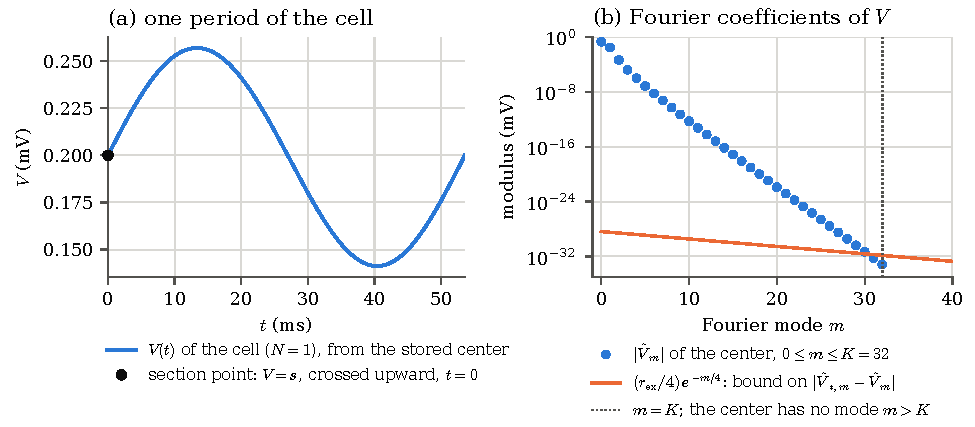
\includegraphics[width=\textwidth]{figures/cell-orbit.pdf}
\caption{The periodic orbit of the cell (Theorem~\ref{thm:cell}). (a) The membrane potential over one period: the $V$ component of the center of the existence proof for $N = 1$ (\texttt{code/\allowbreak fourier/\allowbreak data/\allowbreak centre\_N1\_K32.json}, $K = 32$ modes, hashed by \texttt{data/\allowbreak fourier-existence-N1.json}), summed in binary64 and drawn against $t = \theta/\bar\omega$, with $\bar\omega$ the frequency of the center; the dot is the section point, where $V = s$ is crossed upward, at $t = 0$. The oscillation is small (note the scale of the $V$ axis); it is not an action potential, and nothing is claimed about action potentials. The period is not drawn as data: Theorem~\ref{thm:cell}(ii) encloses it in $[53.58551933936116920991898, 53.58551933936116920991899]$~ms, which lies inside the CAPD enclosure $[53.5855190480139, 53.585519630722438]$~ms of Theorem~\ref{thm:cell}(i). (b) The moduli $|\hat V_m|$ of the Fourier coefficients of $V = 2^{-2}z_V$ in the center (dots, $0 \le m \le K$; the center has no mode $m > K$, dotted line), and the bound $(r_{\mathrm{ex}}/4)e^{-m/4}$ (line), with $r_{\mathrm{ex}}$ the existence radius of Table~\ref{tab:existence} for $N = 1$. By Theorem~\ref{thm:ring}(a) with $N = 1$, to which Theorem~\ref{thm:cell}(ii) refers, the coefficient $\hat V_{*,m}$ of the orbit satisfies $|\hat V_{*,m} - \hat V_m| \le (r_{\mathrm{ex}}/4)e^{-m/4}$ for every $m$, so for $m > K$, $|\hat V_{*,m}|$ is at most this bound; for $m \ge 31$ the stored coefficients are below the bound, so these modes of the center are not resolved individually. Hence the profile $\phi_{*,V}$ differs from the $V$ component of the center (the exact trigonometric polynomial that (a) evaluates in binary64) by at most $r_{\mathrm{ex}}/4$~mV at every phase, and $|\omega_* - \bar\omega| \le r_{\mathrm{ex}}$, far below what the figure can show. A display of stored data, not part of a proof; reproduced by \texttt{code/\allowbreak plot\_cardiac\_rings.py}.}
\label{fig:cell}
\end{figure}

\begin{theorem}[rings; computer-assisted]\label{thm:ring}
Let $G_{Ks} = 0.0275$, $N \in \{8, 16, 32, 64\}$ and $c = N^2/64000$ per ms.
\begin{enumerate}
\item[(a)] (Existence and local uniqueness.) There are $\omega_* > 0$ and a real $2\pi$-periodic $\phi_*$, analytic on the strip $|\im\theta| < 1/4$, with $\phi_{*,V}(0) = s$, such that $x_j(t) = \phi_*(\omega_* t + 2\pi j/N)$ solves \eqref{eq:ring}. The pair $(\omega_*, (a_m)_{m\in\Z})$ formed by $\omega_*$ and the Fourier coefficients of $\Sigma^{-1}\phi_*$ (the profile in the scaled variables of Section~\ref{sec:cell}) lies within $r_{\mathrm{ex}}$ of an explicit center in the norm $\max(|\omega|, \max_k \sum_m |a_{k,m}| e^{|m|/4})$, and it is the only zero of the map \eqref{eq:F} below in the ball of radius $r_{\mathrm{un}}$ about that center, where $r_{\mathrm{un}}$ is the largest double not above $10^{-12}$ ($r_{\mathrm{un}} \approx 9.9999999999999997989 \times 10^{-13}$); $r_{\mathrm{ex}}$ is given in Table~\ref{tab:existence}.
\item[(b)] (Period, minimal period, wave number.) $T = 2\pi/\omega_*$ lies in a certified interval of width less than $2 \times 10^{-25}$~ms (between $1.49 \times 10^{-25}$ and $1.51 \times 10^{-25}$ for the four values of $N$), which Table~\ref{tab:existence} prints rounded outward to 23 decimals. Each cell has minimal period $T$, the solution is not synchronous (it is not the case that $x_j = x_0$ for all $j$), and it is a rotating 1-wave: $x_j(t) = x_0(t + jT/N)$, and no relation $x_j(t) = x_0(t + jkT/N)$ for all $j$ holds with $k \not\equiv 1 \pmod N$.
\item[(c)] (Stability.) Let $\delta = 5764607523035/2^{60} \approx 5.0000000000006636358 \times 10^{-6}$ per ms. The monodromy matrix of the linearization along the wave over the period $T$ has the eigenvalue $1$ algebraically simple, and its other $18N - 1$ eigenvalues (the nontrivial Floquet multipliers, with algebraic multiplicity) have modulus less than $e^{-\delta T}$, which is at most the bound of Table~\ref{tab:stability}. The shift-reduced map $Q^{-1}\varphi_{\tau}$, $\tau = T/N$, has derivative at $x(0)$ with eigenvalue $1$ algebraically simple and all other eigenvalues of modulus less than $e^{-\delta\tau}$. The orbit is locally exponentially orbitally stable with asymptotic phase: for every $\delta' < \delta$ there are $\epsilon_0 > 0$ and $C$ such that every solution starting within distance $\epsilon_0$ of the orbit $O$ satisfies, for some $\sigma \in \R$ and all $t \ge 0$, $|\varphi_t(x^0) - x(t + \sigma)| \le C e^{-\delta' t} \operatorname{dist}(x^0, O)$.
\end{enumerate}
\end{theorem}

Here $\varphi_t$ is the flow of \eqref{eq:ring}. The constants $\epsilon_0$ and $C$ are not computed. Figure~\ref{fig:ring} shows the wave for $N = 8$ and $N = 64$.

\begin{figure}[tbp]
\centering
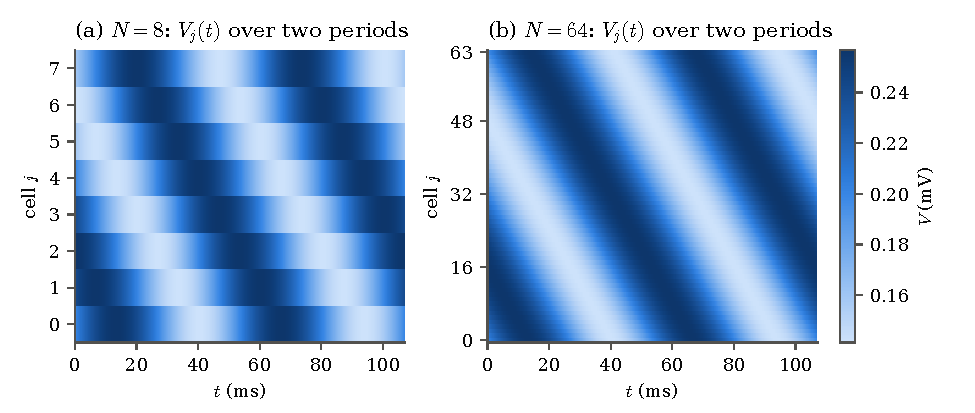
\includegraphics[width=\textwidth]{figures/ring-wave.pdf}
\caption{The rotating 1-wave of Theorem~\ref{thm:ring} on rings of (a) $N = 8$ and (b) $N = 64$ cells: $V_j(t) = \phi_{*,V}(\omega_*t + 2\pi j/N)$, one row per cell $j$, over two periods, $0 \le t \le 2T$, with one color scale for both panels. The profile is the $V$ component of the center of the existence proof for that $N$ (\texttt{code/\allowbreak fourier/\allowbreak data/\allowbreak centre\_N8\_K32.json} and \texttt{centre\_N64\_K32.json}, hashed by \texttt{data/\allowbreak fourier-existence-N8.json} and \texttt{-N64.json}), summed in binary64 at 600 times per row, with the frequency $\bar\omega$ of the center in place of $\omega_*$; by Theorem~\ref{thm:ring}(a) the profile of the wave differs from it by at most $r_{\mathrm{ex}}/4$~mV and $|\omega_* - \bar\omega| \le r_{\mathrm{ex}}$ (Table~\ref{tab:existence}). Since $x_j(t) = x_0(t + jT/N)$, each cell runs $T/N$ ahead of cell $j - 1$, and the crests move toward decreasing $j$, once around the ring in each period. The periods are not drawn as data; Theorem~\ref{thm:ring}(b) encloses them in $[53.58797097681944967415082, 53.58797097681944967415083]$~ms for $N = 8$ and $[53.58810041831757754104213, 53.58810041831757754104214]$~ms for $N = 64$. The figure shows the wave only, not its stability (Theorem~\ref{thm:ring}(c)). Reproduced by \texttt{code/\allowbreak plot\_cardiac\_rings.py}.}
\label{fig:ring}
\end{figure}

\begin{table}[ht]
\centering\small
\begin{tabular}{@{}rlll@{}}
\toprule
$N$ & lower end of the enclosure of $T$ (ms) & $r_{\mathrm{ex}}$ & $Z_1$ \\
\midrule
1 & 53.58551933936116920991898 & $1.7073 \times 10^{-28}$ & 0.20366 \\
8 & 53.58797097681944967415082 & $1.6440 \times 10^{-28}$ & 0.20339 \\
16 & 53.58806910359016923593730 & $1.6415 \times 10^{-28}$ & 0.20338 \\
32 & 53.58809413031803250655154 & $1.6409 \times 10^{-28}$ & 0.20338 \\
64 & 53.58810041831757754104213 & $1.6408 \times 10^{-28}$ & 0.20337 \\
\bottomrule
\end{tabular}
\caption{Existence (Section~\ref{sec:existence}), from the existence records in \texttt{data/}. The printed ends are the exact binary ends stored in the record, about $1.5 \times 10^{-25}$~ms apart, rounded outward to 23 decimals; the upper end is one unit larger in the last printed digit. $r_{\mathrm{ex}}$ and $Z_1$ (both rounded up here) are the radius at which the radii polynomial is negative and the bound of Lemma~\ref{lem:rp}; the uniqueness radius is $r_{\mathrm{un}} \approx 10^{-12}$ for every $N$, set by the validity radius $r_*$ of the bound $Z_2$.}
\label{tab:existence}
\end{table}

\begin{table}[ht]
\centering\small
\begin{tabular}{@{}rlllll@{}}
\toprule
$N$ & bound on $e^{-\delta T}$ (full period) & bound on $e^{-\delta\tau}$ & $K_e$ & $\theta_T$ & worst (SC) ratio \\
\midrule
1 & 0.9978588747123748493822038 & (same) & 16 & 0.2949 & 0.105 \\
8 & 0.9997320960377930203747358 & 0.9999665080790063923613739 & 20 & 0.2817 & 0.090 \\
16 & 0.9997320955472906096505621 & 0.9999832538686231493032797 & 24 & 0.2519 & 0.084 \\
32 & 0.9997320954221904942011761 & 0.9999916268953467731405854 & 32 & 0.2896 & 0.154 \\
64 & 0.9997320953907589193958104 & 0.9999958134384184917812441 & 48 & 0.2951 & 0.170 \\
\bottomrule
\end{tabular}
\caption{Stability (Section~\ref{sec:stability}), from the stability records in \texttt{data/}: the certified upper bounds, rounded upward from Arb, with $\delta = 23058430092137/2^{59}$ per ms for $N = 1$ and $\delta = 5764607523035/2^{60}$ per ms for the rings; the window half-width $K_e$; the tail constant $\theta_T < 1$ of Lemma~\ref{lem:smallgain} (rounded up); and the largest ratio of the left side to the right side of the window inequality (SC) over all window columns, which must be below $1$ (a floating-point figure, the record's \texttt{SC\_worst\_ratio}, rounded up and reported for information; every inequality is decided in Arb).}
\label{tab:stability}
\end{table}

\begin{remark}\label{rem:same}
The CAPD record \file{data/cell-gks0.0275.json} and the Fourier record \file{data/fourier-existence-N1.json} store both period enclosures, and the second lies inside the first; Lemma~\ref{lem:link} shows that the two orbits are the same. An independent computation within the project, by a separate CAPD pipeline that is not part of these proofs, enclosed the periods of the cell in $[53.58551856, 53.58552012]$~ms, of the 8-cell wave in $[53.58795907, 53.58798288]$~ms and of the 16-cell wave in $[53.58805554, 53.58808267]$~ms, with all nontrivial multipliers of modulus below $999/1000$ (cell) and $9999/10000$ (rings). The periods of Theorem~\ref{thm:cell}(ii) and Theorem~\ref{thm:ring} for $N = 1, 8, 16$ lie inside these intervals. We use these intervals as a consistency check only.
\end{remark}

\begin{theorem}[every ring size and the cable; computer-assisted]\label{thm:alln}
Let $G_{Ks} = 0.0275$, and let $d_m(\varepsilon)$, $\mathcal L_\varepsilon$ and $D = 1/64000$ per ms be as in Section~\ref{sec:family}.
\begin{enumerate}
\item[(a)] (One continuous family.) For every $\varepsilon \in [0, 1/64]$ there are $\omega_*(\varepsilon) > 0$ and a real $2\pi$-periodic $\phi_*(\cdot\,;\varepsilon)$ of minimal period $2\pi$, analytic on the strip $|\im\theta| < 1/4$, with $\phi_{*,V}(0;\varepsilon) = s$, that solve \eqref{eq:profile-eps}. Let $x_*(\varepsilon)$ be the pair formed by $\omega_*(\varepsilon)$ and the Fourier coefficients of $\Sigma^{-1}\phi_*(\cdot\,;\varepsilon)$. The map $\varepsilon \mapsto x_*(\varepsilon)$ is continuous from $[0, 1/64]$ into the space $X$ of Section~\ref{sec:F}. Since $x_*(\varepsilon) \in X$, the Fourier series of $\phi_*(\cdot\,;\varepsilon)$ converges absolutely and uniformly on the closed strip $|\im\theta| \le 1/4$, and $\phi_*(\cdot\,;\varepsilon)$ denotes its sum there, a continuous function on the closed strip. The interval $[0, 1/64]$ is covered by 73 pieces, each with an explicit center, and for every piece $P$ that contains $\varepsilon$: $x_*(\varepsilon)$ lies within $9.07 \times 10^{-7}$ of the center of $P$ in the norm of Theorem~\ref{thm:ring}(a); it is the only zero of $F(\cdot\,;\varepsilon)$ (Section~\ref{sec:alln}) within $1.05 \times 10^{-6}$ of that center in that norm, and within $r_{\mathrm{un}}(P) \ge 4.65 \times 10^{-4}$ of it in a weighted norm stored with the piece; and $T(\varepsilon) = 2\pi/\omega_*(\varepsilon)$ lies in an explicit interval of width less than $1.24 \times 10^{-5}$~ms.
\item[(b)] (Every ring size.) For every integer $N \ge 8$, with $c = N^2/64000$ per ms and $\omega_* = \omega_*(1/N^2)$, $x_j(t) = \phi_*(\omega_*t + 2\pi j/N;\, 1/N^2)$ solves \eqref{eq:ring}. Each cell has minimal period $T_N = T(1/N^2)$, the solution is not synchronous, and it is a rotating 1-wave in the sense of Theorem~\ref{thm:ring}(b). It is locally unique in the sense of (a) with $\varepsilon = 1/N^2$, for which $F(\cdot\,;\varepsilon)$ is the map \eqref{eq:F} of this $N$. For $N = 8$, $16$, $32$ and $64$ it is the wave of Theorem~\ref{thm:ring}, and so it is stable in the sense of Theorem~\ref{thm:ring}(c). For every other $N$ its stability is not claimed.
\item[(c)] (The cable.) With $\omega_* = \omega_*(0)$, $u(x, t) = \phi_*(\omega_*t + 2\pi x;\, 0)$, $x \in \R/\Z$, is a real analytic, hence classical, solution of the cable equation \eqref{eq:cable} on the ring of unit length. It is a traveling wave that goes once around the ring in each period $T_\infty = T(0)$, which is its minimal period in $t$ and lies in $[53.58809529823299300232974, 53.58810763684487454838746]$~ms. It is locally unique in the sense of (a) with $\varepsilon = 0$. Its stability is not claimed.
\item[(d)] (The limit $N \to \infty$.) $x_*(1/N^2) \to x_*(0)$ in $X$ as $N \to \infty$. Hence $\phi_*(\cdot\,;1/N^2) \to \phi_*(\cdot\,;0)$ uniformly on the closed strip $|\im\theta| \le 1/4$, and $T_N \to T_\infty$.
\end{enumerate}
\end{theorem}

The pieces, their weights, radii, period enclosures and the SHA-256 of each center are stored in \file{data/fourier-existence-alln.json}, and the exact centers are in its run log \file{code/fourier/data/alln/pieces.jsonl}, whose hash the record stores; Table~\ref{tab:alln} lists the pieces that contain $1/N^2$ for $N = 8, 16, 32, 64$, and the cable. For these four $N$, Theorem~\ref{thm:ring} encloses $T_N$ in intervals about $10^{20}$ times narrower; what Theorem~\ref{thm:alln} adds is every other $N \ge 8$, the cable, and the continuity in $\varepsilon$. It says nothing about a rate of convergence in (d). The proof is in Section~\ref{sec:alln}, and Figure~\ref{fig:alln} draws the pieces.

\begin{table}[ht]
\centering\small
\begin{tabular}{@{}lllll@{}}
\toprule
$N$ & piece $P$ & enclosure of $T_N$ from $P$ (ms) & left side of \eqref{eq:incl} & $r_{\mathrm{un}}(P)$ \\
\midrule
8 & $[63/4096, 1/64]$ & $[53.58796640015, 53.58797756550]$ & $6.90 \times 10^{-7}$ & $4.86 \times 10^{-4}$ \\
16 & $[63/16384, 67/16384]$ & $[53.58806282472, 53.58807434393]$ & $3.57 \times 10^{-7}$ & $4.86 \times 10^{-4}$ \\
32 & $[7/8192, 9/8192]$ & $[53.58808831963, 53.58809994100]$ & $1.31 \times 10^{-11}$ & $4.85 \times 10^{-4}$ \\
64 & $[0, 1/4096]$ & $[53.58809529823, 53.58810763685]$ & $7.25 \times 10^{-7}$ & $4.65 \times 10^{-4}$ \\
64 & $[7/32768, 15/32768]$ & $[53.58809380464, 53.58810545862]$ & $5.40 \times 10^{-7}$ & $6.06 \times 10^{-4}$ \\
$\infty$ (cable) & $[0, 1/4096]$ & $[53.58809529823, 53.58810763685]$ & -- & $4.65 \times 10^{-4}$ \\
\bottomrule
\end{tabular}
\caption{Theorem~\ref{thm:alln} at the ring sizes of Theorem~\ref{thm:ring} and for the cable, from \texttt{data/\allowbreak fourier-existence-alln.json}. The period enclosures are the record's outward-rounded decimal ends, rounded outward again to 11 decimals; each contains the enclosure of Table~\ref{tab:existence} for the same $N$. The fourth column (rounded up) is the left side of the inclusion \eqref{eq:incl} of the existence ball of Theorem~\ref{thm:ring}(a) in the uniqueness ball of $P$, which must not exceed $r_{\mathrm{un}}(P)$ (rounded down); $1/4096$ lies in two pieces, and both inclusions hold. Theorem~\ref{thm:ring} gives no ball for the cable, so its entry is empty.}
\label{tab:alln}
\end{table}

\begin{theorem}[single-cell conductance family; computer-assisted]\label{thm:conductance}
Let $N=1$, $g=G_{Ks}$ and $J=[0.027499735464,0.02778996093]$~nS/pF, for the model of Section~\ref{sec:model}. The exact source-bound numerical inequalities of Sections~\ref{sec:conductance-methods} and~\ref{sec:hopf-methods} are verified by the records specified in Section~\ref{sec:conductance-gates}.
\begin{enumerate}
\item[(a)] For every $g\in J$ there is a real nonconstant cell profile $\phi_*(\cdot;g)$, analytic on $|\im\theta|<1/4$, and a positive frequency $\omega_*(g)$ such that $z(t)=\phi_*(\omega_*(g)t;g)$ solves the scaled cell equation. Its voltage first harmonic is real and nonzero. The pair of frequency and Fourier coefficients is continuous in the weighted Fourier space, locally Lipschitz on each of the 712 pieces, lies in that piece's existence ball and is its only phase-fixed zero in the uniqueness ball. The profile has minimal period $2\pi$, and $T(g)=2\pi/\omega_*(g)$ is the minimal physical period. The 711 adjacent inclusions identify one branch on all of $J$.
\item[(b)] The accepted uniform stability units cover all of $J$. On each unit $I_u$ let $\delta_u>0$ and $\omega_{{\rm hi},u}$ be the certified bounds. For every $g\in I_u$, the Floquet multiplier $1$ is algebraically simple, and the other 17 multipliers satisfy
\[
 |\lambda|<e^{-\delta_u T(g)}\le e^{-\delta_u T_{{\rm lo},u}}<1,
 \qquad T_{{\rm lo},u}=2\pi/\omega_{{\rm hi},u}.
\]
The orbit is locally exponentially orbitally stable with asymptotic phase. For each fixed $g$ and $0<\delta'<\delta_u$, nonlinear constants $C_g,\epsilon_g>0$ exist as in Theorem~\ref{thm:ring}(c); these constants and the neighborhood size are not computed or claimed uniform in $g$. All 63 admitted units use $\delta_u=3\times10^{-5}$ per ms; taking the maximum of their outward multiplier bounds gives $|\lambda|\le0.998413816$ for every nontrivial multiplier throughout $J$.
\item[(c)] There is a supercritical Hopf point $(z_H,g_H,\omega_H)$ and a continuous normalized family
\[
 z_\varepsilon(t)=c(\varepsilon)+\varepsilon w(\omega(\varepsilon)t;\varepsilon),
 \qquad 0\le\varepsilon\le6427/50000,
\]
with $g(0)=g_H$, $c(0)=z_H$, $\omega(0)=\omega_H>0$ and $w_{V,1}=w_{V,-1}=1/2$ in the fixed scaled TP06 coordinates. Thus $a_{1,V}=\varepsilon/2$ there and $|\widehat V_1|=\varepsilon/8$~mV in physical voltage. Its positive-amplitude solutions are nonconstant, have minimal period $2\pi/\omega(\varepsilon)$, and are locally unique in their normalized enclosures. The 68 amplitude pieces and 67 adjacent inclusions form one continuous family. A fresh existence proof at $g_s=0.02778$ identifies an orbit common to this family and (a). Their connected union contains a periodic orbit at every conductance in $[\inf J,g_H)$ and the Hopf equilibrium at its endpoint. Sufficiently small positive amplitudes have the local orbital stability supplied by the classical Hopf theorem. No monotonicity of $g(\varepsilon)$, global uniqueness at a fixed conductance, explicit size of that Hopf neighborhood, or uniform stability on the entire amplitude bridge is asserted.
\end{enumerate}
\end{theorem}

This extension concerns only the single cell. The all-$N$ and cable assertions of Theorem~\ref{thm:alln} retain their fixed conductance and their original stability scope. Historical pointwise stability successes are not used as a substitute for the new uniform cover. The numerical evidence and its acceptance checks are specified in Section~\ref{sec:conductance-gates}.

\begin{figure}[p]
\centering
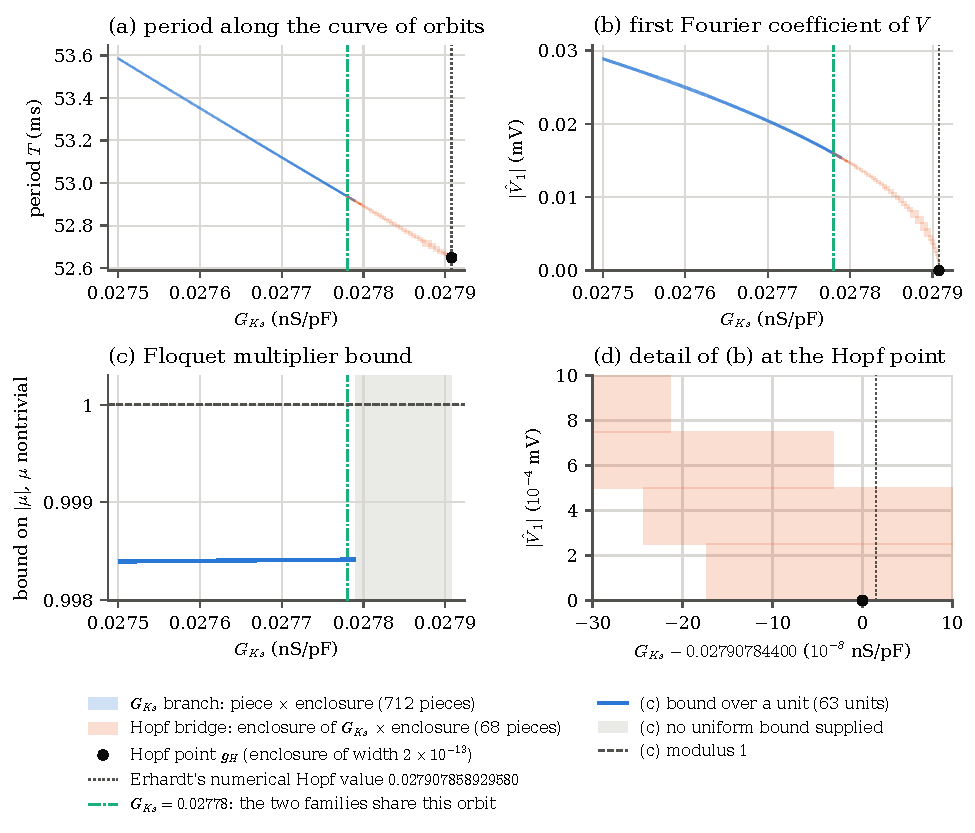
\includegraphics[width=\textwidth]{figures/branch-hopf.pdf}
\caption{The single-cell conductance family and its amplitude bridge to the Hopf point. Panels (a) and (b) show the stored period and physical first-voltage-harmonic enclosures for all 712 conductance pieces (blue) and all 68 freshly re-proved amplitude pieces (orange). Overlapping rectangles enclose families, rather than sampled numerical trajectories. The green line marks the fresh common orbit at $G_{Ks}=0.02778$. Panel (c) shows the outward nontrivial Floquet multiplier bound over each of the 63 uniform certificates. The gray interval has no supplied quantitative uniform bound; local Hopf attraction does not fill that interval with a numerical decay estimate. Panel (d) enlarges the endpoint enclosures. The black marker displays the certified Hopf interval, whose width is below the plotting resolution. Erhardt's printed numerical Hopf value is shown separately and lies outside that interval. Legends lie outside the data panels. All plotted values are rounded to binary64 for display; the proofs use the stored exact or interval values.}
\label{fig:branch}
\end{figure}

\section{Existence in Fourier space}\label{sec:existence}

\subsection{Rigorous Fourier coefficients of a composition}\label{sec:fe}

Let $p(\theta) = \sum_{|m| \le K} a_m e^{im\theta}$ with $a_m \in \C^n$ given as complex balls; every statement below holds for every trigonometric polynomial with coefficients in the balls. Let $f: U \to \C^q$ be holomorphic on an open $U \subset \C^n$, given by an inclusion function $\mathsf F$: a program that maps a list of complex balls $X$ to balls $Y$ or raises an error, such that whenever all of $Y$ is finite, $X \subset U$ and $f(z) \in Y$ for every $z \in X$. A program written with $+, -, \times$, integer powers, $\exp$, division, and logarithms and square roots that raise unless their argument ball lies in $\{\re w > 0\}$ is such an inclusion function, with $U$ the set on which every divisor is nonzero and every logarithm and square-root argument has positive real part, by induction over the expression. (Arb returns a non-finite ball for a quotient whose divisor ball contains $0$; Arb's own complex logarithm does not signal a ball that crosses the branch cut, which is why the guards are needed.) Let $g = f \circ p$, $c_k = \frac{1}{2\pi}\int_0^{2\pi} g(\theta) e^{-ik\theta}\,d\theta$, and $\Sigma_\rho = \{\theta \in \C : |\im\theta| \le \rho\}$.

\begin{lemma}[strip cover]\label{lem:strip}
Cover the rectangle $R = [0, 2\pi] \times [-\rho, \rho]$ by finitely many closed rectangles $B = [2\pi x_1, 2\pi x_2] \times [\rho y_1, \rho y_2]$ with exact rationals $x_i, y_i$ (the proof uses only that the rectangles cover $R$). For each $B$ let $\Theta_B$ be a complex ball containing $B$, $P_B = \sum_m a_m \exp(i m \Theta_B)$ evaluated in ball arithmetic, and $Y_B = \mathsf F(P_B)$. If every $Y_B$ is finite, then $p(\Sigma_\rho) \subset U$, $g$ is holomorphic on an open neighborhood of $\Sigma_\rho$, and $\sup_{\Sigma_\rho} |g_i| \le S_i := \max_B \overline{|Y_{B,i}|}$, where $\overline{|\cdot|}$ is an upper bound of the modulus.
\end{lemma}

\begin{proof}
Every $\theta \in R$ lies in some $B$, so $p(\theta) \in P_B \subset U$ by the inclusion property. Since $p$ is $2\pi$-periodic, $p(\Sigma_\rho) = p(R) \subset U$; as $U$ is open and $p$ continuous, $p^{-1}(U)$ is an open set containing $\Sigma_\rho$, on which $g$ is holomorphic. Finally $|g_i(\theta)| \le \overline{|Y_{B,i}|} \le S_i$.
\end{proof}

The whole rectangle is covered, not only its edges: a pole of $g$ strictly inside the strip can coexist with a finite supremum on the edges, and then the next lemma fails. The programs refine the cover adaptively and optionally use a centered (mean-value) form on each box; both only affect how tight $S$ is.

\begin{lemma}[Cauchy estimate]\label{lem:cauchy}
If $g$ is holomorphic on an open set containing $\Sigma_\rho$, $2\pi$-periodic, and $|g| \le S$ on $\Sigma_\rho$, then $|c_m| \le S e^{-\rho|m|}$ for every $m \in \Z$.
\end{lemma}

\begin{proof}
For $m > 0$ integrate $g(\theta)e^{-im\theta}$ over the boundary of the rectangle with corners $0, 2\pi, 2\pi - i\rho, -i\rho$. The integral vanishes by Cauchy's theorem and the vertical sides cancel by periodicity, so $c_m = \frac{1}{2\pi}\int_0^{2\pi} g(x - i\rho)e^{-im(x - i\rho)}\,dx$ and $|e^{-im(x - i\rho)}| = e^{-m\rho}$. For $m < 0$ shift to $\im\theta = \rho$; $|c_0| \le S$ directly.
\end{proof}

\begin{lemma}[aliasing]\label{lem:alias}
Under the hypotheses of Lemma~\ref{lem:cauchy}, with $\hat c_k = \frac1M \sum_{j=0}^{M-1} g(2\pi j/M) e^{-2\pi ijk/M}$ and $|k| < M$,
\[ |\hat c_k - c_k| \le E_k := S\,\frac{e^{-\rho(M - k)} + e^{-\rho(M + k)}}{1 - e^{-\rho M}}. \]
\end{lemma}

\begin{proof}
By Lemma~\ref{lem:cauchy} $\sum_m |c_m| < \infty$, so the Fourier series converges absolutely and uniformly to $g$. Substituting and using $\frac1M\sum_j e^{2\pi ij(m-k)/M} = 1$ if $m \equiv k \pmod M$ and $0$ otherwise gives $\hat c_k = \sum_{l\in\Z} c_{k + lM}$. For $l \ge 1$, $k + lM > 0$ and $\sum_{l \ge 1}|c_{k+lM}| \le S e^{-\rho(M+k)}/(1 - e^{-\rho M})$; for $l = -j \le -1$, $|k - jM| = jM - k$ and the sum is at most $S e^{-\rho(M-k)}/(1 - e^{-\rho M})$.
\end{proof}

\begin{proposition}[enclosure of the coefficients]\label{prop:enclosure}
Let the strip cover succeed with bounds $S_i$. Evaluate the nodes $e^{im\theta_j}$, $\theta_j = 2\pi j/M$, as balls ($e^{i\pi q}$ for exact rationals $q$), $P_j = \sum_m a_m e^{im\theta_j}$ and $G_j = \mathsf F(P_j)$, and let $C_k = \frac1M\sum_j G_j e^{-ik\theta_j} + E_k\,([-1,1] + i[-1,1])$. Then for every $p$ with coefficients in the balls, every component $i$ and every $|k| \le K' < M$, $c_{i,k}[f \circ p] \in C_{i,k}$, and $|c_{i,m}| \le S_i e^{-\rho|m|}$ for every $m$.
\end{proposition}

\begin{proof}
The ball sum contains $\hat c_k$, and a complex number $w$ with $|w| \le E_k$ lies in the square $E_k([-1,1] + i[-1,1])$. Lemmas~\ref{lem:strip} to~\ref{lem:alias}.
\end{proof}

For $\nu > 0$ with $q = \nu e^{-\rho} < 1$ these bounds give the weighted tail $\sum_{|m| > K'} |c_m|\nu^{|m|} \le 2S q^{K'+1}/(1 - q)$.

\subsection{The zero-finding problem}\label{sec:F}

Fix $K = 32$ and a center $\bar x = (\bar\omega, \bar a)$ of exact dyadic numbers, with $\bar a_m = 0$ for $|m| > K$, $\bar a_{-m} = \overline{\bar a_m}$ and $\bar\omega$ real; it is computed by an untrusted Newton iteration (\file{code/fourier/centre.py}) and stored in \file{code/fourier/data/centre_N*_K32.json}. Let $\nu = e^{1/4}$, let $\ell^1_\nu$ be the sequences $(b_m)_{m\in\Z}$ with $\|b\|_\nu = \sum_m |b_m|\nu^{|m|} < \infty$, a Banach algebra under convolution, and let $X = \C \times (\ell^1_\nu)^{18}$ with $\|x\| = \max(|\omega|, \max_k \|a_k\|_\nu)$ (the programs allow weights; all runs of Stage~E used weight $1$, and Section~\ref{sec:alln} uses weights). Writing $\phi_a(\theta) = \sum_m a_m e^{im\theta}$, $g(a) = f \circ \phi_a$ and $g_m(a)$ for its Fourier coefficients, define $F$, on the open set of $x \in X$ for which $\phi_a$ maps the closed strip $|\im\theta| \le 1/4$ into the domain $U$ (it contains the ball $B_{r_*}(\bar x)$ used below, Section~\ref{sec:Z2}), with values in $X' := \C \times (\ell'_\nu)^{18}$, by
\begin{equation}\label{eq:F}
  F_{\mathrm{ph}}(x) = \sum_m a_{m,V} - s/\sigma_V, \qquad F_m(x) = i\omega m a_m - g_m(a) + d_m E a_m \quad (m \in \Z),
\end{equation}
where $\sigma_V = 2^{-2}$ is the scale of $V$, so $F_{\mathrm{ph}} = 0$ says $\phi_{a,V}(0) = s$ in physical units. Here $\ell'_\nu$ is the space of sequences with $\|b\|' = \sum_m |b_m|\nu^{|m|}/(1 + |m|) < \infty$, and $X'$ has the norm $\max(|\cdot|, \max_k\|\cdot\|')$; $F$ maps $X$ into $X'$ because $(i\omega ma_m)_m \in \ell'_\nu$ when $a \in \ell^1_\nu$, and $g(a)$, $d_mEa_m \in \ell^1_\nu \subset \ell'_\nu$. A zero of $F$ with $\omega > 0$ and $\phi_a$ real and $C^1$ solves \eqref{eq:profile}, and the phase condition removes the time-shift invariance.

\subsection{The radii-polynomial theorem}\label{sec:rp}

Let $A: X' \to X$ be an injective bounded linear operator, defined below, and $\Psi(x) = x - AF(x)$, a map from $X$ to $X$. Its fixed points are exactly the zeros of $F$.

\begin{lemma}[radii polynomial]\label{lem:rp}
Let $r_* > 0$ be such that $\Psi$ is defined and $C^1$ on the closed ball $B_{r_*}(\bar x)$, and suppose that
\[ \|AF(\bar x)\| \le Y_0, \qquad \|I - A\,DF(\bar x)\| \le Z_1, \qquad \|A(DF(x) - DF(\bar x))\| \le Z_2 \|x - \bar x\| \ \ (x \in B_{r_*}(\bar x)). \]
If $0 < r \le r_*$, $p(r) := Y_0 + (Z_1 - 1)r + Z_2 r^2/2 < 0$ and $Z_1 + Z_2 r < 1$, then $\Psi$ maps $B_r(\bar x)$ into itself and is a contraction there, so $F$ has exactly one zero in $B_r(\bar x)$.
\end{lemma}

\begin{proof}
$\|D\Psi(x)\| \le Z_1 + Z_2\|x - \bar x\|$. For $x \in B_r(\bar x)$, $\|\Psi(x) - \bar x\| \le \|\Psi(\bar x) - \bar x\| + \|\int_0^1 D\Psi(\bar x + t(x - \bar x))(x - \bar x)\,dt\| \le Y_0 + Z_1 r + Z_2 r^2/2 < r$. The mean value inequality on the convex ball gives the contraction constant $Z_1 + Z_2 r < 1$, and Banach's fixed point theorem gives one fixed point, which is a zero of $F$ since $A$ is injective.
\end{proof}

The programs check $p(r) < 0$ and $Z_1 + Z_2 r < 1$ in Arb at two exact dyadic radii: the small radius $r_{\mathrm{ex}}$ of Table~\ref{tab:existence}, which places the zero, and $r_{\mathrm{un}}$, the largest double not above $r_* = 10^{-12}$, which gives uniqueness (the contraction constant there is about $0.267$). The validity radius $r_*$ is chosen by hand, so $r_{\mathrm{un}}$ is not an optimal uniqueness radius.

\subsection{The operator \texorpdfstring{$A$}{A} and its tail}\label{sec:A}

Let $J(\theta) = Df(\phi_{\bar a}(\theta)) = \sum_n J_n e^{in\theta}$. The derivative $DF(\bar x)y$, $y = (y_\omega, (y_m))$, has phase component $\sum_m y_{m,V}$ and row $m$ equal to $iy_\omega m\bar a_m + i\bar\omega m y_m - \sum_n J_n y_{m-n} + d_m E y_m$. The operator $A$ is block diagonal with respect to the finite part (the phase row and modes $|m| \le K$, with the unknown $\omega$) and each tail mode $|m| > K$:
\begin{itemize}
\item $A_{\mathrm{fin}}$, an exact complex matrix of size $1 + 18(2K + 1)$, the floating-point inverse of the midpoint of the Galerkin matrix $J_{\mathrm{fin}}$ (the restriction of $DF(\bar x)$ to these rows and columns);
\item $A_m = (i\bar\omega m I - \hat J_0 + d_m E)^{-1}$ for $|m| > K$, where $\hat J_0$ is the exact real midpoint of the enclosure of $J_0$.
\end{itemize}
$A$ acts on $X'$ block by block. It is bounded from $X'$ to $X$ because $\sup_{|m| > K}(1 + |m|)|A_m| < \infty$ (Lemma~\ref{lem:Atail}), and it is injective because every block is: every $A_m$ is an inverse, and $A_{\mathrm{fin}}$ is invertible, which follows from $\|I - A_{\mathrm{fin}}J_{\mathrm{fin}}\| \le Z_1 < 1$, since the compression of $I - A\,DF(\bar x)$ to the finite modes is $I - A_{\mathrm{fin}}J_{\mathrm{fin}}$ and the coordinate projection onto the finite modes has norm 1 in $X$. Since $\hat J_0$ and $d_m$ are real, $A_{-m} = \overline{A_m}$, and only $m > 0$ is computed.

\begin{lemma}[tail of $A$]\label{lem:Atail}
For $K < m \le m_{\max}$ the matrices $A_m$ are enclosed by Arb inversion of a ball matrix whose only non-exact entries are the narrow balls of $d_m$ (exact for $N = 1$); Arb raises unless every matrix in the ball is certainly invertible, and otherwise returns a ball containing every inverse. Let $G_0 = |\hat J_0| + 4c\,E$ entrywise, $\Upsilon = \bar\omega(m_{\max} + 1)$, $G = G_0/\Upsilon$ and $\vartheta = \|G\|_\infty < 1$. Then for every $m > m_{\max}$, entrywise,
\[ |A_m| \le \frac{1}{\Upsilon} S_G, \qquad |mA_m| \le \frac{1}{\bar\omega} S_G, \qquad S_G := I + G + G^2 + \frac{\vartheta^3}{1 - \vartheta}\,\one\one^{\mathsf T}. \]
\end{lemma}

\begin{proof}
With $y = \bar\omega m \ge \Upsilon$ and $B_0 = \hat J_0 - d_m E$, $|B_0| \le G_0$ entrywise because $0 \le d_m \le 4c$. Then $A_m = (iy)^{-1}(I - B_0/(iy))^{-1} = (iy)^{-1}\sum_k (B_0/(iy))^k$, and entrywise $|A_m| \le y^{-1}\sum_k (G_0/y)^k \le \Upsilon^{-1}\sum_k G^k$. Each entry of $G^k$ is at most the corresponding row sum of $G^k$, which is at most $\vartheta^k$; summing over $k \ge 3$ gives the last term. Finally $|mA_m| = (y/\bar\omega)|A_m| \le \bar\omega^{-1}\sum_k (G_0/y)^k$.
\end{proof}

The program increases $m_{\max}$ until $\vartheta \le 1/2$ is certified ($m_{\max} = 391$ at $N = 8$, and between $391$ and $395$ over the five runs of Table~\ref{tab:existence}). The suprema $\bar A_0 = \sup_{|m| > K}|A_m|$, $\bar A_1 = \sup_{|m| > K}|mA_m|$ and $C_n = \sup_{|m| > K}|A_m J'_n|$, with $J'_n = J_n$ for $n \ne 0$ and $J'_0 = J_0 - \hat J_0$, are taken entrywise over both ranges; for $|n| \le 12$, $C_n$ is the entrywise maximum of the explicit products $|A_mJ'_n|$ over $K < m \le m_{\max}$ and of the bound $\Upsilon^{-1}S_G|J'_n| \ge |A_m||J'_n|$ valid for every $m > m_{\max}$; for $12 < |n| \le K'$, $C_n = \bar A_0|J'_n|$. Negative $m$ are handled by $A_{-m}J'_n = \overline{A_m \overline{J'_n}}$.

\subsection{The bounds \texorpdfstring{$Y_0$}{Y0} and \texorpdfstring{$Z_1$}{Z1}}\label{sec:Y0Z1}

The Fourier data come from Proposition~\ref{prop:enclosure}: enclosures of $g_m(\bar a)$ and $J_n$ for $|m|, |n| \le K' = 2K + 16 = 80$ from an $M = 192$ node transform, with strip suprema $S_g$ and (entrywise) $S_J$ on $|\im\theta| \le \rho = 3/2$, and beyond $K'$ the bounds $|g_{k,m}| \le S_{g,k}e^{-\rho|m|}$, $|J_{n,jk}| \le S_{J,jk}e^{-\rho|n|}$. Let $q = \nu e^{-\rho} < 1$. For a linear operator $B$ on $X$ with blocks $B_{cc'}$, $\|B\| \le \max_c \sum_{c'}\|B_{cc'}\|$ with $\|B_{cc'}\|_{\ell^1_\nu \to \ell^1_\nu} = \sup_{m'}\sum_m |B(m,m')|\nu^{|m|}/\nu^{|m'|}$ (the column supremum).

\paragraph{$Y_0$.} The finite part of $AF(\bar x)$ is $A_{\mathrm{fin}}F_{\mathrm{fin}}(\bar x)$, computed in Arb. For $|m| > K$, $\bar a_m = 0$ and $F_m(\bar x) = -g_m$, so $(AF)_m = -A_m g_m$. For $K < |m| \le K'$ the computed enclosures of $A_m$ are used (all of them are explicit, since $m_{\max} \ge 391 > K' = 80$ in every run of Table~\ref{tab:existence}), and for $|m| > K'$, entrywise $|A_mg_m| \le \bar A_0 S_g e^{-\rho|m|}$, so $\sum_{|m| > K'}|(A_mg_m)_c|\nu^{|m|} \le \sum_k(\bar A_0)_{ck}S_{g,k}\,2q^{K'+1}/(1 - q)$. Then $Y_0 = \max_c\big(\|(AF)_{c,\mathrm{fin}}\|_\nu + \|(AF)_{c,\mathrm{tail}}\|_\nu\big)$, the phase/$\omega$ component counting as a component with the single mode $0$.

\paragraph{$Z_1$.} Let $B = I - A\,DF(\bar x)$. Finite rows and finite columns give $I - A_{\mathrm{fin}}J_{\mathrm{fin}}$, an Arb matrix product. A tail column $(k, m')$, $|m'| > K$, meets the finite rows through $-A_{\mathrm{fin}}w$, where $w$ has phase entry $1$ if $k = V$ and $0$ otherwise (the phase functional sums over all modes) and row $(j, m)$ entry $-J_{m-m',jk}$ (the terms $i\bar\omega m$ and $d_m$ vanish off the diagonal $m = m'$); for $K < |m'| \le K + 16$ the enclosures of $J$ are used, and for $|m'| \ge K + 17$ the bound $|J_{m-m',jk}| \le S_{J,jk}e^{-\rho(|m'| - \operatorname{sgn}(m')m)}$ makes every term of the weighted column sum divided by $\nu^{|m'|}$ a constant times $\nu^{-|m'|}$ or $(e^{-\rho}/\nu)^{|m'|}$, both decreasing in $|m'|$, so the value at $|m'| = K + 17$ bounds the supremum. For the tail rows, since $A_m(i\bar\omega m - \hat J_0 + d_m E) = I$,
\[ (By)_m = A_m\Big[(J_0 - \hat J_0)y_m + \sum_{n\ne0} J_n y_{m-n}\Big] = \sum_n A_m J'_n y_{m-n} \qquad (|m| > K), \]
($y_\omega$ does not enter because $\bar a_m = 0$ there), and $\nu^{|m|} \le \nu^{|m-n|}\nu^{|n|}$ gives $\|(By)_{c,\mathrm{tail}}\|_\nu \le \sum_k \mathcal T_{ck}\|y_k\|_\nu$ with $\mathcal T = \sum_{|n| \le K'} C_n\nu^{|n|} + \bar A_0 S_J\, 2q^{K'+1}/(1 - q)$, for every column. For an output component $c$ and an input component $c'$ let $f\!f_{cc'}$ be the largest weighted column sum of the finite rows of block $(c, c')$ over the finite columns, and $f\!t_{cc'}$ the same over the tail columns (bounded as above). A column of $B$ meets the finite rows and the tail rows, so its weighted sum in block $(c,c')$ is at most $\max(f\!f_{cc'}, f\!t_{cc'}) + \mathcal T_{cc'}$, and
\[ Z_1 = \max_c\sum_{c'}\big(\max(f\!f_{cc'}, f\!t_{cc'}) + \mathcal T_{cc'}\big). \]
The $\omega$ column has a single finite column and no tail rows ($iy_\omega m\bar a_m = 0$ for $|m| > K$), and the $\omega$ row of $B$ (the output of the phase column of $A_{\mathrm{fin}}$) has no tail part, since $A$ has no tail in that row, so for it only the finite-row terms enter.

\subsection{The bound \texorpdfstring{$Z_2$}{Z2} by a polydisc majorant}\label{sec:Z2}

Let $R_k = 1/1024$ for every component, and let $M_k$ be the strip supremum (Lemma~\ref{lem:strip}, on $|\im\theta| \le \rho_2 = 1$) of $f_k$ over the family of trigonometric polynomials obtained from $\phi_{\bar a}$ by replacing each constant coefficient $\bar a_{0,j}$ by the complex box of half-width $R_j$ about it. Since that box contains the disc of radius $R_j$, $M_k \ge \sup\{|f_k(\phi_{\bar a}(\theta) + w)| : |\im\theta| \le 1, |w_j| \le R_j\}$, and the finite cover certifies that $f$ is holomorphic on an open set containing these points.

\begin{lemma}\label{lem:Z2}
Let $q_2 = \nu e^{-\rho_2} < 1$ and $Q_2 = (1 + q_2)/(1 - q_2)$. For $h \in (\ell^1_\nu)^{18}$ with $\|h_j\|_\nu < R_j$, the map $a \mapsto g_k(a)$ is analytic at $\bar a + h$ and
\[ \|D^2 g_k(\bar a + h)[u, v]\|_\nu \le \sum_{j,l}\partial_j\partial_l\Phi_k(\|h\|)\,\|u_j\|_\nu\|v_l\|_\nu, \qquad \Phi_k(t) = M_k Q_2\prod_j (1 - t_j/R_j)^{-1}. \]
\end{lemma}

\begin{proof}
For $|\im\theta| \le 1$ the Taylor coefficients $c_\alpha(\theta) = \partial^\alpha f_k(\phi_{\bar a}(\theta))/\alpha!$ satisfy $|c_\alpha(\theta)| \le M_k R^{-\alpha}$ by Cauchy's inequality on the closed polydisc, and they are holomorphic and $2\pi$-periodic in $\theta$; Lemma~\ref{lem:cauchy} gives $|[c_\alpha]_m| \le M_k R^{-\alpha}e^{-|m|}$ and so $\|c_\alpha\|_\nu \le M_k R^{-\alpha}Q_2$. In the Banach algebra $\ell^1_\nu$ the series $\sum_\alpha c_\alpha h^\alpha$ (convolution powers) converges absolutely, dominated by $\Phi_k(\|h\|)$. For real $\theta$, $|h_j(\theta)| \le \|h_j\|_\nu < R_j$, so the Taylor series of $f_k$ at $\phi_{\bar a}(\theta)$ converges to $f_k(\phi_{\bar a}(\theta) + h(\theta))$; convergence in $\ell^1_\nu$ is uniform convergence, so the two functions agree and $g_k(\bar a + h) = \sum_\alpha c_\alpha h^\alpha$. Differentiating termwise and comparing with the majorant, whose coefficients are nonnegative, gives the bound.
\end{proof}

For $x = \bar x + \Delta$ with $\|\Delta\| \le r$ and $\|y\| \le 1$,
\[ (DF(x) - DF(\bar x))y = im(y_\omega\,\Delta a_m + \Delta\omega\,y_m) - (Dg(\bar a + \Delta a) - Dg(\bar a))y_a. \]
The first term $b = y_\omega\Delta a + \Delta\omega\,y_a$ has $\|b_k\|_\nu \le 2r$, and $\|A(imb)\|_c \le \sum_k (N_1 + \bar A_1)_{ck}\|b_k\|$, with $N_1$ the block norms of $A_{\mathrm{fin}}\operatorname{diag}(im)$. The second equals $\int_0^1 D^2g(\bar a + t\Delta a)[\Delta a, y_a]\,dt$, whose component $k$ has norm at most $rW_k(r)$ with
\[ W_k(r) = M_kQ_2P(r)\Big[\Big(\sum_j s_j\Big)^2 + \sum_j s_j^2\Big], \qquad s_j = \frac{1}{R_j - r}, \quad P(r) = \prod_j\frac{R_j}{R_j - r}, \]
because $\partial_jP = P/(R_j - t_j)$, $\partial_l\partial_jP = P/((R_j - t_j)(R_l - t_l))$ for $j \ne l$ and $2P/(R_j - t_j)^2$ for $j = l$, and $\Phi_k$ is increasing. Hence
\[ Z_2 = \max_c\sum_k\big[2(N_1 + \bar A_1)_{ck} + (N_0 + \bar A_0)_{ck}W_k(r_*)\big], \]
with $N_0$ the block norms of $A_{\mathrm{fin}}$ on the coefficient columns; in the $\omega$ row only $N_0$ and $N_1$ enter. $\Psi$ is defined and $C^1$ on $B_{r_*}(\bar x)$ because $r_* < R_j$, $g$ is analytic there, the term $A(i\omega ma_m)$ is a bounded bilinear map ($\sup_{|m| > K}|m||A_m| < \infty$ by Lemma~\ref{lem:Atail}), and the other terms are bounded linear.

\subsection{The real solution, its period and its wave number}\label{sec:real}

\begin{lemma}\label{lem:real}
Let the hypotheses of Lemma~\ref{lem:rp} hold at $r_{\mathrm{ex}}$ and $r_{\mathrm{un}}$, let $\bar\omega - r_{\mathrm{ex}} > 0$, and let $x_* = (\omega_*, a_*)$ be the zero. Then $\omega_*$ is real and positive, $\phi_* = \phi_{a_*}$ is real-valued, analytic on $|\im\theta| < 1/4$, and solves \eqref{eq:profile}. If also $|\bar a_{1,V}| > r_{\mathrm{ex}}/\nu$, then $\phi_*$ has minimal period $2\pi$, and for $N \ge 2$ the ring solution $x_j(t) = \phi_*(\omega_*t + 2\pi j/N)$ has minimal period $T = 2\pi/\omega_*$, is not synchronous and is a rotating 1-wave in the sense of Theorem~\ref{thm:ring}(b).
\end{lemma}

\begin{proof}
Let $\kappa(\omega, a) = (\operatorname{conj}\omega, (\operatorname{conj} a_{-m})_m)$, an isometry of $X$ with $\kappa(\bar x) = \bar x$. The program \file{code/fourier/tp06_18d_arb.py} that evaluates $f$ is a fixed composition of $+, -, \times, /$, integer powers, 55 exponentials, 4 logarithms and 3 square roots with real constants, and contains no absolute value, real or imaginary part, comparison, branch or conversion. Each of these operations commutes with complex conjugation wherever it is defined: the arithmetic operations algebraically, $\exp$ because its power series has real coefficients, and the principal logarithm and square root on $\{\re w > 0\}$, the only arguments admitted, because that set is invariant under conjugation and $\operatorname{Log}\bar w = \overline{\operatorname{Log} w}$, $\sqrt{\bar w} = \overline{\sqrt w}$ there. By induction over the expression, if $z$ lies in the domain then so does $\bar z$, and $f(\bar z) = \overline{f(z)}$. The points used are $\phi_{\bar a}(\theta) + h(\theta)$ with $\theta$ real and $|h_j(\theta)| < R_j$; this family is closed under conjugation ($\phi_{\bar a}(\theta)$ is real) and lies in the certified domain. Hence $g_m(\kappa a) = \overline{g_{-m}(a)}$, and since $d_{-m} = d_m$ and $s/\sigma_V$ are real, $F(\kappa x) = \overline{F(x)}$ in the corresponding sense; so $\kappa$ maps zeros of $F$ in $B_{r_{\mathrm{un}}}(\bar x)$ to zeros in the same ball, and uniqueness gives $\kappa x_* = x_*$: $\omega_*$ is real and $\phi_*$ is real-valued. As $a_* \in (\ell^1_\nu)^{18}$, $\phi_*$ is analytic on $|\im\theta| < 1/4$; since $i\omega_* m a_{*,m} = g_m - d_m E a_{*,m}$, the coefficient sequence of $\phi_*'$ is in $\ell^1_\nu$, and \eqref{eq:profile} holds pointwise. $\omega_* \ge \bar\omega - r_{\mathrm{ex}} > 0$ by hypothesis.

Since $\|a_{*,V} - \bar a_V\|_\nu \ge \nu|a_{*,1,V} - \bar a_{1,V}|$, $|a_{*,1,V} - \bar a_{1,V}| \le r_{\mathrm{ex}}/\nu$, so $a_{*,1,V} \ne 0$. A function of minimal period $2\pi/k$, $k \ge 2$, has $a_m = 0$ unless $k \mid m$; hence $\phi_*$ has minimal period $2\pi$ and each cell has minimal period $T$. A synchronous solution would make $\phi_*$ periodic with period $2\pi/N$. If $x_j(t) = x_0(t + jkT/N)$ for all $j$ and some $k \not\equiv 1 \pmod N$, then with $j = 1$, $\phi_*(\theta + 2\pi/N) = \phi_*(\theta + 2\pi k/N)$, so $\phi_*$ would have the period $2\pi(k-1)/N \not\equiv 0 \pmod{2\pi}$, contradicting minimality.
\end{proof}

\begin{proof}[Proof of Theorem~\ref{thm:ring}(a), (b) and the existence part of Theorem~\ref{thm:cell}(ii)]
For each $N \in \{1, 8, 16, 32, 64\}$ the program \file{code/fourier/existence.py} computes, in Arb, the strip covers (all leaves finite, full strip), the enclosures of Proposition~\ref{prop:enclosure}, the tail of Lemma~\ref{lem:Atail}, $Y_0$, $Z_1$ and $Z_2$ as above, checks $p(r) < 0$ and $Z_1 + Z_2r < 1$ at $r = r_{\mathrm{ex}}$ and at $r = r_{\mathrm{un}} \le r_*$, checks $\bar\omega - r_{\mathrm{ex}} > 0$, and $|\bar a_{1,V}| > r_{\mathrm{ex}}/\nu$, and writes the interval $2\pi/[\omega_*]$ with outward-rounded decimal ends. The records \file{data/fourier-existence-N*.json} store every bound; for example at $N = 8$: $Y_0 = 1.3096 \times 10^{-28}$, $Z_1 = 0.20339$, $Z_2 \le 6.4002 \times 10^{10}$,\allowbreak $|\bar a_{1,V}| \ge 0.11524$. Lemmas~\ref{lem:rp} and~\ref{lem:real} give the statements.
\end{proof}

\subsection{Every ring size and the cable}\label{sec:alln}

This subsection proves Theorem~\ref{thm:alln}. The parameter is $\varepsilon$ of Section~\ref{sec:family}, and $G_{Ks} = 0.0275$ is fixed.

\paragraph{Zeros of the family.} For $\varepsilon \ge 0$ let $F(x;\varepsilon)$ have the components \eqref{eq:F} with $d_m$ replaced by $d_m(\varepsilon)$ of \eqref{eq:deps}: the phase component $F_{\mathrm{ph}}(x)$ and $F_m(x;\varepsilon) = i\omega ma_m - g_m(a) + d_m(\varepsilon)Ea_m \in \C^{18}$, $m \in \Z$, defined for every $x = (\omega, a) \in X$ for which $\phi_a$ maps the closed strip $|\im\theta| \le 1/4$ into $U$. We call $x$ a zero of $F(\cdot\,;\varepsilon)$ if all these components vanish. For $\varepsilon = 1/N^2$ these are the components of the map \eqref{eq:F} of the $N$-ring, and a zero in the sense of Section~\ref{sec:F} is a zero in this sense. For $\varepsilon > 0$, $d_m(\varepsilon) \le 4D/\varepsilon$ is bounded in $m$; for $\varepsilon = 0$, $d_m(0)a_m$ grows like $m^2a_m$, and $F(\cdot\,;0)$ need not take values in $X'$. We therefore work with a fixed-point map that is defined without a codomain for $F$.

\paragraph{Pieces.} A piece is an interval $P = [\varepsilon_{\mathrm{lo}}, \varepsilon_{\mathrm{hi}}]$ with exact dyadic ends, $0 \le \varepsilon_{\mathrm{lo}} < \varepsilon_{\mathrm{hi}}$, midpoint $\varepsilon_c$ and half-width $\delta_P$. On a piece we fix $K = 12$ and: a center $\bar x = (\bar\omega, \bar a)$ of exact dyadic numbers, with $\bar\omega > 0$, $\bar a_m = 0$ for $|m| > K$ and $\bar a_{-m} = \overline{\bar a_m}$ (an untrusted Newton iterate at $\varepsilon_c$); weights $\eta = (\eta_\omega, \eta_1, \dots, \eta_{18})$, exact dyadic numbers in $(0, 1]$, and the norm $\|x\|_\eta = \max(|\omega|/\eta_\omega, \max_k\|a_k\|_\nu/\eta_k)$ on $X$; $A_{\mathrm{fin}}$, the floating-point inverse of the midpoint of the Galerkin matrix of Section~\ref{sec:A} at $\bar x$ with the damping $d_m(\varepsilon_c)$; $\hat J_0$ as in Section~\ref{sec:A}; and, for $|m| > K$ and $\varepsilon \in P$, $A_m(\varepsilon) = (i\bar\omega mI - \hat J_0 + d_m(\varepsilon)E)^{-1}$. Since every weight is at most $1$, $\|x\| \le \|x\|_\eta$, and a weight depends only on the component, so the conjugation $\kappa$ of the proof of Lemma~\ref{lem:real} is an isometry of $\|\cdot\|_\eta$. For $\varepsilon \in P$ define $T_\varepsilon(x)$ by
\begin{equation}\label{eq:Teps}
  T_\varepsilon(x)_{\mathrm{fin}} = x_{\mathrm{fin}} - A_{\mathrm{fin}}F_{\mathrm{fin}}(x;\varepsilon), \qquad T_\varepsilon(x)_m = -A_m(\varepsilon)\big[i(\omega - \bar\omega)ma_m + \hat J_0a_m - g_m(a)\big] \quad (|m| > K),
\end{equation}
where $x_{\mathrm{fin}}$ collects $\omega$ and the modes $|m| \le K$, and $F_{\mathrm{fin}}$ the phase component and the $F_m$ with $|m| \le K$.

\begin{lemma}[tail resolvents for every damping]\label{lem:tailT}
Let $\hat J_0$ be a real $18 \times 18$ matrix, $\bar\omega > 0$, $m_{\max} \ge 1$, $\Upsilon = \bar\omega(m_{\max} + 1)$, $G = |\hat J_0|/\Upsilon$ entrywise, $\vartheta = \|G\|_\infty < 1$, and $S_G$ as in Lemma~\ref{lem:Atail}. Then for every integer $m > m_{\max}$ and every real $d \ge 0$ the matrix $M = i\bar\omega mI - \hat J_0 + dE$ is invertible and, entrywise,
\[ |M^{-1}| \le S_G/\Upsilon, \qquad |mM^{-1}| \le S_G/\bar\omega. \]
For $m < -m_{\max}$ the same bounds hold with $|m|$, since $M$ is then the complex conjugate of the matrix for $-m$.
\end{lemma}

\begin{proof}
Let $y = \bar\omega m \ge \Upsilon$ and let $\Lambda_y$ be the diagonal matrix with entry $iy + d$ in the position of $V$ and $iy$ elsewhere, so $M = \Lambda_y - \hat J_0$. As $d$ is real, $|iy + d| \ge y$, so $|\Lambda_y^{-1}| \le I/y$ entrywise and $\|\Lambda_y^{-1}\hat J_0\|_\infty \le \|\hat J_0\|_\infty/y \le \vartheta < 1$. Hence $M^{-1} = \sum_{k\ge0}(\Lambda_y^{-1}\hat J_0)^k\Lambda_y^{-1}$ and, entrywise, $|M^{-1}| \le y^{-1}\sum_k(|\hat J_0|/y)^k \le \Upsilon^{-1}\sum_kG^k \le S_G/\Upsilon$, the last step as in the proof of Lemma~\ref{lem:Atail}. Since $m/y = 1/\bar\omega$, $|mM^{-1}| \le \bar\omega^{-1}\sum_k(|\hat J_0|/y)^k \le S_G/\bar\omega$.
\end{proof}

Unlike Lemma~\ref{lem:Atail}, this needs no upper bound on the damping, so it covers $d_m(0) = 4\pi^2Dm^2$. For $K < m \le m_{\max}$ the program encloses the range of $d_m$ over $P$ in an exact interval $[d_{\mathrm{lo}}, d_{\mathrm{hi}}] \subset [0, \infty)$ (by evaluating \eqref{eq:deps} on the hull of $P$), covers it by finitely many balls of width about $\bar\omega m/4$, and encloses $A_m$ on each ball by Arb inversion of the ball matrix (as in Lemma~\ref{lem:Atail}), so that every $A_m(\varepsilon)$, $\varepsilon \in P$, lies in one of these enclosures. The suprema $\bar A_0$, $\bar A_1$ and $C_n$ of Section~\ref{sec:A} are then taken over $|m| > K$ and $\varepsilon \in P$, with the maximum over these enclosures in the explicit range and Lemma~\ref{lem:tailT} beyond it.

\begin{lemma}[the fixed-point map]\label{lem:Teps}
Let $P$ be a piece, $\varepsilon \in P$, and $B$ a closed ball about $\bar x$ such that, for $x \in B$, $\phi_a$ maps the closed strip $|\im\theta| \le 1/4$ into $U$ and $a \mapsto g(a)$ is of class $C^1$ from $B$ into $(\ell^1_\nu)^{18}$. Suppose that $\bar A_0$ and $\bar A_1$ are finite and that $A_{\mathrm{fin}}$ is invertible. Then $T_\varepsilon$ maps $B$ into $X$ and is of class $C^1$ there, and $T_\varepsilon(x) = x$ if and only if $x$ is a zero of $F(\cdot\,;\varepsilon)$. The derivative $DT_\varepsilon(\bar x)$ has the finite rows of $I - A_{\mathrm{fin}}\,DF_{\mathrm{fin}}(\bar x;\varepsilon)$ and the tail rows $(DT_\varepsilon(\bar x)y)_m = \sum_nA_m(\varepsilon)J'_ny_{m-n}$, $|m| > K$, with $J'_n$ as in Section~\ref{sec:A}; it is the operator $I - A\,DF(\bar x)$ of Section~\ref{sec:Y0Z1} with $d_m(\varepsilon)$ and $A_m(\varepsilon)$ in place of $d_m$ and $A_m$. Finally, $DT_\varepsilon(x) - DT_\varepsilon(\bar x)$ is obtained by applying $-A_{\mathrm{fin}}$ and $-A_m(\varepsilon)$ to the rows of $DF(x;\varepsilon) - DF(\bar x;\varepsilon)$, which do not contain $d_m(\varepsilon)$.
\end{lemma}

\begin{proof}
The finite part of $T_\varepsilon$ involves the phase component, a bounded linear functional on $X$, and finitely many $F_m$, each a $C^1$ function of $x$ on $B$. The tail part is the sum of $-(A_m(\varepsilon)i(\omega - \bar\omega)ma_m)_m$, a bilinear map of $(\omega - \bar\omega, a)$ bounded because $|mA_m(\varepsilon)| \le \bar A_1$ entrywise, and of the bounded linear maps $a \mapsto -(A_m(\varepsilon)\hat J_0a_m)_m$ and $b \mapsto (A_m(\varepsilon)b_m)_m$, the latter applied to $g(a)$; so $T_\varepsilon$ is of class $C^1$ from $B$ into $X$. For $|m| > K$, the identity $A_m(\varepsilon)(i\bar\omega m - \hat J_0 + d_m(\varepsilon)E) = I$ gives $a_m - T_\varepsilon(x)_m = A_m(\varepsilon)F_m(x;\varepsilon)$, and $x_{\mathrm{fin}} - T_\varepsilon(x)_{\mathrm{fin}} = A_{\mathrm{fin}}F_{\mathrm{fin}}(x;\varepsilon)$; as $A_{\mathrm{fin}}$ and every $A_m(\varepsilon)$ are invertible, $T_\varepsilon(x) = x$ if and only if every component of $F(x;\varepsilon)$ vanishes. Differentiating the tail part at $\bar x$ in a direction $y$, with $\omega = \bar\omega$ and $\bar a_m = 0$ for $|m| > K$, gives $-A_m(\varepsilon)[\hat J_0y_m - \sum_nJ_ny_{m-n}] = \sum_nA_m(\varepsilon)J'_ny_{m-n}$. In $DF(x;\varepsilon) - DF(\bar x;\varepsilon)$ the term $d_m(\varepsilon)Ey_m$ cancels, and the tail part of $DT_\varepsilon(x) - DT_\varepsilon(\bar x)$ is $-A_m(\varepsilon)$ applied to $i(\omega - \bar\omega)my_m + iy_\omega ma_m - [(Dg(a) - Dg(\bar a))y_a]_m$.
\end{proof}

\begin{lemma}[the derivative of $d_m$]\label{lem:dd}
$d'_m(\varepsilon) = 8\pi^4Dm^4S(w)S'(w)$ with $w = \pi^2m^2\varepsilon$ and $S'(w) = \sum_{k\ge1}(-1)^kkw^{k-1}/(2k+1)!$, and $S'(w) = (\cos\sqrt w - S(w))/(2w)$ for $w > 0$. If $0 \le w \le W$, $n \ge 1$, $q_n = W/((2n+2)(2n+3)) < 1$ and $q'_n = W/(2n(2n+3)) < 1$, then $S(w)$ and $S'(w)$ differ from their partial sums over $k < n$ by at most $t_n/(1 - q_n)$ and $u_n/(1 - q'_n)$, with $t_n = W^n/(2n+1)!$ and $u_n = nW^{n-1}/(2n+1)!$.
\end{lemma}

\begin{proof}
The derivative is the chain rule applied to \eqref{eq:deps}, and the closed form follows by differentiating $\sin\sigma/\sigma$, $\sigma = \sqrt w$. The $k$-th terms of the two series have moduli at most $t_k$ and $u_k$, and for $k \ge n$, $t_{k+1}/t_k = W/((2k+2)(2k+3)) \le q_n$ and $u_{k+1}/u_k = W/(2k(2k+3)) \le q'_n$, so the tails are dominated by geometric series.
\end{proof}

The program covers $P$ by subintervals with exact rational ends, evaluates $S$ and $S'$ on the corresponding balls of $w$ in Arb (the partial sums with these remainders, or the closed forms where $w > 1$ is certain), and takes the union of the resulting enclosures of $d'_m$: a real ball $DD_m$ that contains $d'_m(\xi)$ for every $\xi \in P$, for each $|m| \le K$.

\begin{lemma}[bounds uniform over a piece]\label{lem:uniform}
Let $P$ be a piece and, for $|m| \le K$, $DD_m$ a real interval containing $d'_m(\xi)$ for every $\xi \in P$. For each output component $c$ (the $\omega$ component or one of the 18 state components) let $Y^{\mathrm p}_{0,c}$ be the bound of Section~\ref{sec:Y0Z1} for the component $c$ of $AF(\bar x)$, computed with $d_m(\varepsilon_c)$ in the finite rows and with the tail suprema over $|m| > K$ and $\varepsilon \in P$; let $Y^{\mathrm g}_{0,c}$ bound $\|(A_{\mathrm{fin}}w)_c\|_\nu$ for every $w$ in the box $W$ whose only nonzero entries are $W_{(V,m)} = DD_m\,\bar a_{V,m}$, $|m| \le K$; let $B_{1,cc'} = \max(f\!f_{cc'}, f\!t_{cc'}) + \mathcal T_{cc'}$ be the block bounds of Section~\ref{sec:Y0Z1}, computed with $d_m(\varepsilon_c)$ in the finite block and with the tail suprema over $P$; and let
\[ B^{\mathrm g}_{1,cV} = \max_{|m|\le K}\frac{\overline{|DD_m|}}{\nu^{|m|}}\sum_{(j,m')\in c}|(A_{\mathrm{fin}})_{(j,m'),(V,m)}|\,\nu^{|m'|}, \qquad B^{\mathrm g}_{1,cc'} = 0 \ (c' \ne V), \]
the sum over the rows of component $c$. Then for every $\varepsilon \in P$
\[ \|T_\varepsilon(\bar x) - \bar x\|_\eta \le Y_0 := \max_c\frac{Y^{\mathrm p}_{0,c} + \delta_PY^{\mathrm g}_{0,c}}{\eta_c}, \qquad \|DT_\varepsilon(\bar x)\|_\eta \le Z_1 := \max_c\frac1{\eta_c}\sum_{c'}\eta_{c'}\big(B_{1,cc'} + \delta_PB^{\mathrm g}_{1,cc'}\big). \]
\end{lemma}

\begin{proof}
An operator $B$ on $X$ with blocks $B_{cc'}$ has $\|B\|_\eta \le \max_c\eta_c^{-1}\sum_{c'}\eta_{c'}\|B_{cc'}\|$, since $\|y_{c'}\| \le \eta_{c'}\|y\|_\eta$. By the mean value theorem for the real function $d_m$, $d_m(\varepsilon) - d_m(\varepsilon_c) = (\varepsilon - \varepsilon_c)d'_m(\xi_m)$ for some $\xi_m \in P$, and $|\varepsilon - \varepsilon_c| \le \delta_P$. In $F_{\mathrm{fin}}(\bar x;\varepsilon)$ only the entries $(V, m)$ contain the damping, so $F_{\mathrm{fin}}(\bar x;\varepsilon) = F_{\mathrm{fin}}(\bar x;\varepsilon_c) + (\varepsilon - \varepsilon_c)w$ with $w_{(V,m)} = d'_m(\xi_m)\bar a_{V,m}$, $w \in W$, and $\|(A_{\mathrm{fin}}F_{\mathrm{fin}}(\bar x;\varepsilon))_c\|_\nu \le \|(A_{\mathrm{fin}}F_{\mathrm{fin}}(\bar x;\varepsilon_c))_c\|_\nu + \delta_PY^{\mathrm g}_{0,c}$. The tail components of $T_\varepsilon(\bar x) - \bar x$ are $A_m(\varepsilon)g_m(\bar a)$, bounded as in Section~\ref{sec:Y0Z1} because the suprema are taken over $\varepsilon \in P$. For $Z_1$, by Lemma~\ref{lem:Teps}: in the finite block, $I - A_{\mathrm{fin}}J_{\mathrm{fin}}(\varepsilon) = [I - A_{\mathrm{fin}}J_{\mathrm{fin}}(\varepsilon_c)] - A_{\mathrm{fin}}\Delta(\varepsilon)$, where $\Delta(\varepsilon)$ is diagonal with the entries $d_m(\varepsilon) - d_m(\varepsilon_c)$ on the coordinates $(V, m)$ and $0$ elsewhere; column $(V, m)$ of $A_{\mathrm{fin}}\Delta(\varepsilon)$ is column $(V, m)$ of $A_{\mathrm{fin}}$ times a number of modulus at most $\delta_P\overline{|DD_m|}$, so its weighted column sum over the rows of $c$, divided by $\nu^{|m|}$, is at most $\delta_PB^{\mathrm g}_{1,cV}$. The finite rows of the tail columns contain no damping (it acts on the diagonal, in tail rows) and are bounded as in Section~\ref{sec:Y0Z1}. The tail rows are $\sum_nA_m(\varepsilon)J'_ny_{m-n}$ and are bounded by $\mathcal T$ with the suprema over $P$.
\end{proof}

\begin{lemma}[$Z_2$ from a bound on the Hessian]\label{lem:hess}
Let $R_1, \dots, R_{18} > 0$ and $\rho_2 > 1/4$ with $q_2 = \nu e^{-\rho_2} < 1$, $Q_2 = (1 + q_2)/(1 - q_2)$. Suppose that $f$ is holomorphic on an open set containing the compact set $\mathcal K = \{\phi_{\bar a}(\theta) + w : |\im\theta| \le \rho_2,\ |w_i| \le R_i\}$ and that $|\partial_j\partial_lf_k| \le M\!H_{kjl}$ on $\mathcal K$. Write $J_{kj} = \partial_jf_k$, $H_{kjl} = \partial_j\partial_lf_k$, and for $a \in (\ell^1_\nu)^{18}$ with $t_i := \|a_i - \bar a_i\|_\nu < R_i$ let $\Pi(t) = \prod_iR_i/(R_i - t_i)$. Then:
\begin{enumerate}
\item[(a)] $\phi_a$ maps the closed strip $|\im\theta| \le 1/4$ into $\mathcal K$, $g(a)$, $J_{kj}\circ\phi_a$ and $H_{kjl}\circ\phi_a$ lie in $\ell^1_\nu$, and $\|H_{kjl}\circ\phi_a\|_\nu \le M\!H_{kjl}Q_2\Pi(t)$;
\item[(b)] $a \mapsto g(a)$ and $a \mapsto J_{kj}\circ\phi_a$ are of class $C^1$ into $\ell^1_\nu$, with $(Dg(a)y)_k = \sum_j(J_{kj}\circ\phi_a)*y_j$ and $D(J_{kj}\circ\phi_a)h = \sum_l(H_{kjl}\circ\phi_a)*h_l$, where $*$ is the convolution product;
\item[(c)] if $\eta_ir_* < R_i$ for every $i$, then for every $\varepsilon \in P$ and every $x$ with $\|x - \bar x\|_\eta \le r \le r_*$, $\|DT_\varepsilon(x) - DT_\varepsilon(\bar x)\|_\eta \le Z_2r$, where
\[ Z_2 := \max_c\frac1{\eta_c}\sum_k\big[2\eta_\omega\eta_k(N_1 + \bar A_1)_{ck} + (N_0 + \bar A_0)_{ck}W_k\big], \qquad W_k := Q_2\,\Pi(\eta r_*)\sum_{j,l}\eta_j\eta_l\,M\!H_{kjl}, \]
$N_0$ and $N_1$ are the block norms of Section~\ref{sec:Z2}, $\bar A_0$ and $\bar A_1$ the suprema over $|m| > K$ and $\varepsilon \in P$, and $\Pi(\eta r_*)$ is $\Pi$ at $t_i = \eta_ir_*$; in the $\omega$ row only $N_0$ and $N_1$ enter.
\end{enumerate}
\end{lemma}

\begin{proof}
(a) For $|\im\theta| \le 1/4$, $|\phi_{a,i}(\theta) - \phi_{\bar a,i}(\theta)| \le t_i < R_i$, so $\phi_a(\theta) \in \mathcal K$. The rest is the proof of Lemma~\ref{lem:Z2} with $H_{kjl}$, $J_{kj}$ and $f_k$ in place of $f_k$: for $|\im\theta| \le \rho_2$ the Taylor coefficients $c_\alpha(\theta)$ of $w \mapsto H_{kjl}(\phi_{\bar a}(\theta) + w)$ satisfy $|c_\alpha(\theta)| \le M\!H_{kjl}R^{-\alpha}$ by Cauchy's inequality on the closed polydisc of radii $R$, they are holomorphic and $2\pi$-periodic in $\theta$, and Lemma~\ref{lem:cauchy} gives $\|c_\alpha\|_\nu \le M\!H_{kjl}R^{-\alpha}Q_2$; so with $h = a - \bar a$ the series $\sum_\alpha c_\alpha h^\alpha$ (convolution powers) converges absolutely in $\ell^1_\nu$, with norm at most $M\!H_{kjl}Q_2\prod_i(1 - t_i/R_i)^{-1}$, and its sum is $H_{kjl}\circ\phi_a$ because for real $\theta$ the Taylor series converges to $H_{kjl}(\phi_a(\theta))$ and convergence in $\ell^1_\nu$ is uniform convergence. For $J_{kj}$ and $f_k$ the same holds with bounds of $|J_{kj}|$ and $|f_k|$ on the compact set $\mathcal K$. (b) A power series in $h$ with coefficients in the Banach algebra $\ell^1_\nu$, dominated as above by a scalar power series in $(t_i)$ with nonnegative coefficients that converges for $t_i < R_i$, defines a $C^1$ map on $\{t_i < R_i\}$ whose derivative is obtained by differentiating term by term, because the series of the derivatives of the terms is dominated by the derivatives of the scalar series, which converge locally uniformly on the same set; the term-by-term derivative of the series of $f_k$ (of $J_{kj}$) in the direction $h_j$ ($h_l$) is the series of $J_{kj}$ ($H_{kjl}$) applied to $h_j$ ($h_l$), since the Taylor coefficients of $\partial_jf_k$ are those of $f_k$ differentiated. (c) By Lemma~\ref{lem:Teps}, $DT_\varepsilon(x) - DT_\varepsilon(\bar x)$ applies $-A$ to $(DF(x;\varepsilon) - DF(\bar x;\varepsilon))y = (im(y_\omega\Delta a_m + \Delta\omega\,y_m))_m - (Dg(\bar a + \Delta a) - Dg(\bar a))y_a$, with $\Delta = x - \bar x$. For $\|y\|_\eta \le 1$, component $k$ of $b = y_\omega\Delta a + \Delta\omega\,y_a$ has norm at most $|y_\omega|\|\Delta a_k\|_\nu + |\Delta\omega|\|y_k\|_\nu \le 2\eta_\omega\eta_kr$, and $\|(A(imb))_c\| \le \sum_k(N_1 + \bar A_1)_{ck}\|b_k\|_\nu$ as in Section~\ref{sec:Z2}. By (b) and the mean value inequality along the segment $\bar a + \sigma\Delta a$, $\sigma \in [0, 1]$, on which $t_i \le \eta_ir \le \eta_ir_* < R_i$,
\[ \big\|[(Dg(\bar a + \Delta a) - Dg(\bar a))y_a]_k\big\|_\nu \le \sum_{j,l}\sup_\sigma\|H_{kjl}\circ\phi_{\bar a + \sigma\Delta a}\|_\nu\,\|\Delta a_l\|_\nu\|y_j\|_\nu \le rW_k, \]
because $\Pi$ increases in each $t_i$; applying $A$ costs $(N_0 + \bar A_0)_{ck}$. Dividing by $\eta_c$ gives the claim.
\end{proof}

The program computes $M\!H$ (\file{code/fourier/branch.py}, class \texttt{HessBound}) as the strip supremum of Lemma~\ref{lem:strip}, on $|\im\theta| \le \rho_2 = 1$, of the second derivatives of $f$ over the family of trigonometric polynomials obtained from $\phi_{\bar a}$ by replacing each constant coefficient $\bar a_{0,i}$ by the complex box of half-width $R_i$ about it, where $R_i$ is an exact dyadic number close to $32\eta_ir_*$ (the program checks $\eta_ir_* < R_i$), a family that contains $\phi_{\bar a}(\theta) + w$ for $|w_i| \le R_i$. The second derivatives are evaluated with second-order forward-mode dual numbers in Arb; every intermediate is checked to be finite and every logarithm and square-root argument to lie in $\{\re w > 0\}$, so that, by the induction of Section~\ref{sec:fe} applied to the value, gradient and Hessian of each intermediate, a finite result encloses $f$, $Df$ and $D^2f$ and certifies that $f$ is holomorphic on an open set containing $\mathcal K$.

\begin{lemma}[continuity and gluing]\label{lem:glue}
(a) Let $P$ be a piece and $0 < r_{\mathrm{ex}} \le r_{\mathrm{un}} \le r_*$ such that, for every $\varepsilon \in P$, $T_\varepsilon$ maps $B_{r_{\mathrm{ex}}}(\bar x)$ into itself and is a contraction with constant $L < 1$ on $B_{r_{\mathrm{un}}}(\bar x)$ (balls of $\|\cdot\|_\eta$), and let $x_*(\varepsilon)$ be its fixed point in $B_{r_{\mathrm{ex}}}(\bar x)$, which is its only fixed point in $B_{r_{\mathrm{un}}}(\bar x)$. Then $\varepsilon \mapsto x_*(\varepsilon)$ is continuous from $P$ into $X$.
(b) Let $P_a$ and $P_b$ be pieces as in (a) with $P_a \cap P_b \ne \emptyset$ and
\begin{equation}\label{eq:glue}
  \|\bar x_a - \bar x_b\|_{\eta(b)} + r_{\mathrm{ex}}(a)\max_c\frac{\eta_c(a)}{\eta_c(b)} \le r_{\mathrm{un}}(b).
\end{equation}
Then $x_{*,a} = x_{*,b}$ on $P_a \cap P_b$.
\end{lemma}

\begin{proof}
(a) For $\varepsilon, \varepsilon' \in P$ both fixed points lie in $B_{r_{\mathrm{un}}}(\bar x)$, where $T_{\varepsilon'}$ is a contraction with constant $L$, so
\begin{align*}
\|x_*(\varepsilon') - x_*(\varepsilon)\|_\eta &\le \|T_{\varepsilon'}(x_*(\varepsilon')) - T_{\varepsilon'}(x_*(\varepsilon))\|_\eta + \|T_{\varepsilon'}(x) - T_\varepsilon(x)\|_\eta\\
&\le L\|x_*(\varepsilon') - x_*(\varepsilon)\|_\eta + \|T_{\varepsilon'}(x) - T_\varepsilon(x)\|_\eta
\end{align*}
with $x = x_*(\varepsilon)$. It remains to show that $\varepsilon' \mapsto T_{\varepsilon'}(x)$ is continuous at $\varepsilon$ for this fixed $x = (\omega, a)$. The finite part changes by $A_{\mathrm{fin}}$ applied to the finitely many terms $(d_m(\varepsilon') - d_m(\varepsilon))Ea_m$, $|m| \le K$. The tail part changes by $-(A_m(\varepsilon') - A_m(\varepsilon))v_m$, $v_m = i(\omega - \bar\omega)ma_m + \hat J_0a_m - g_m(a)$; each term tends to $0$, as $A_m(\cdot)$ is the inverse of a continuous family of invertible matrices, and entrywise $|(A_m(\varepsilon') - A_m(\varepsilon))v_m| \le 2\bar A_1|\omega - \bar\omega||a_m| + 2\bar A_0|\hat J_0a_m - g_m(a)|$, which is summable with the weights $\nu^{|m|}$; dominated convergence gives the claim.
(b) Since $\|y\|_{\eta(b)} \le \|y\|_{\eta(a)}\max_c\eta_c(a)/\eta_c(b)$, for $\varepsilon \in P_a \cap P_b$ the point $x_{*,a}(\varepsilon)$ lies in the closed ball of radius $r_{\mathrm{un}}(b)$ about $\bar x_b$ in $\|\cdot\|_{\eta(b)}$. It is a zero of $F(\cdot\,;\varepsilon)$ by Lemma~\ref{lem:Teps}, hence a fixed point of the map $T_\varepsilon$ of $P_b$ in that ball, so it is $x_{*,b}(\varepsilon)$.
\end{proof}

\begin{proof}[Proof of Theorem~\ref{thm:alln}]
\emph{The computation.} The program \file{code/fourier/alln.py} proves the 73 pieces of the record \file{data/fourier-existence-alln.json}. Each has width $1/4096$; consecutive pieces overlap by $1/32768$, the first starts at $0$ and the last ends at $1/64$. For each piece it computes in Arb, with $K = 12$, $K' = 2K + 16 = 40$, $M = 128$ nodes, $\rho = 3/2$ and $\rho_2 = 1$ (the settings and the working precisions are stored in the record): the strip covers and the enclosures of Proposition~\ref{prop:enclosure} at the center, the balls $DD_m$ of Lemma~\ref{lem:dd}, the tail data of Lemma~\ref{lem:tailT}, the bounds $Y_0$ and $Z_1$ of Lemma~\ref{lem:uniform}, and the Hessian cover and $Z_2$ of Lemma~\ref{lem:hess} with $R_i$ close to $32\eta_ir_*$; it checks $\vartheta < 1$, $\eta_ir_* < R_i$, $p(r) < 0$ and $Z_1 + Z_2r < 1$ at $r = r_{\mathrm{ex}}$ and at $r = r_{\mathrm{un}} \le r_*$, $\bar\omega - \eta_\omega r_{\mathrm{ex}} > 0$ and $|\bar a_{1,V}| > \eta_Vr_{\mathrm{ex}}/\nu$, and stores the period interval $2\pi/[\bar\omega - \eta_\omega r_{\mathrm{ex}}, \bar\omega + \eta_\omega r_{\mathrm{ex}}]$ with outward-rounded decimal ends. Over the 73 pieces: $Y_0$ lies between $6.90 \times 10^{-7}$ and $7.26 \times 10^{-7}$, almost all of it the term $\delta_PY^{\mathrm g}_0$ of the parameter width (the part at $\varepsilon_c$ is at most $7.42 \times 10^{-11}$); $Z_1$ lies between $0.152$ and $0.199$, $Z_2$ between $1305$ and $1373$, $r_{\mathrm{ex}}$ between $8.14 \times 10^{-7}$ and $9.07 \times 10^{-7}$, $r_{\mathrm{un}}$ between $4.65 \times 10^{-4}$ and $6.11 \times 10^{-4}$, and $Z_1 + Z_2r_{\mathrm{un}} \le 0.979$; $m_{\max} = 391$ and $\vartheta < 0.4964$ on every piece; the weights lie in $[0.00216, 1]$, with $\eta_V = 1$; the period intervals are narrower than $1.24 \times 10^{-5}$~ms.

\emph{Each piece.} Fix a piece and $\varepsilon \in P$. By Lemma~\ref{lem:hess}(a), (b), Lemma~\ref{lem:Teps} applies on the ball $B_{r_*}(\bar x)$ of $\|\cdot\|_\eta$ ($\|a_i - \bar a_i\|_\nu \le \eta_ir_* < R_i$ there), once $A_{\mathrm{fin}}$ is known to be invertible; that follows from $Z_1 < 1$ as in Section~\ref{sec:A}, since the compression of $DT_\varepsilon(\bar x)$ to the finite coordinates is $I - A_{\mathrm{fin}}J_{\mathrm{fin}}(\varepsilon)$ and the coordinate projection has norm $1$ for $\|\cdot\|_\eta$. With Lemmas~\ref{lem:uniform} and~\ref{lem:hess}(c), the proof of Lemma~\ref{lem:rp}, which uses only the three bounds and Banach's fixed point theorem, shows that $T_\varepsilon$ maps $B_{r_{\mathrm{ex}}}(\bar x)$ into itself and is a contraction there and on $B_{r_{\mathrm{un}}}(\bar x)$, with constant at most $Z_1 + Z_2r_{\mathrm{un}} < 1$; so $T_\varepsilon$ has exactly one fixed point $x_*(\varepsilon)$ in $B_{r_{\mathrm{un}}}(\bar x)$, it lies in $B_{r_{\mathrm{ex}}}(\bar x)$, and by Lemma~\ref{lem:Teps} it is the only zero of $F(\cdot\,;\varepsilon)$ in $B_{r_{\mathrm{un}}}(\bar x)$. The proof of Lemma~\ref{lem:real} applies to it with $\|\cdot\|_\eta$ (for which $\kappa$ is an isometry), with $d_m(\varepsilon)$ real and even in $m$, with the domain certified by the Hessian cover (the points $\phi_{\bar a}(\theta) + h(\theta)$, $\theta$ real, $|h_j(\theta)| < R_j$), and with the checks $\bar\omega - \eta_\omega r_{\mathrm{ex}} > 0$ and $|\bar a_{1,V}| > \eta_Vr_{\mathrm{ex}}/\nu$: $\omega_*(\varepsilon)$ is real and positive, $\phi_*(\cdot\,;\varepsilon)$ is real, analytic on $|\im\theta| < 1/4$ and of minimal period $2\pi$, $\phi_{*,V}(0;\varepsilon) = s$, and $T(\varepsilon)$ lies in the stored interval. It solves \eqref{eq:profile-eps} pointwise: the coefficient sequences of $\phi_*$, $\phi_*'$, $\phi_*''$ and $f(\phi_*)$ are absolutely summable (as $|m|^j\nu^{-|m|}$ is bounded), the shifts in $\mathcal L_\varepsilon$ act on mode $m$ by $e^{\pm2\pi imh}$, and the vanishing of every $F_m(x_*;\varepsilon)$ is the equality of the Fourier coefficients of the two sides. By Lemma~\ref{lem:glue}(a), $x_*$ is continuous on $P$.

\emph{Gluing.} The program checks that the lower ends and the upper ends of the pieces increase strictly and that $r_{\mathrm{ex}} < r_{\mathrm{un}}$ on each piece; only consecutive pieces overlap (the record lists no other overlap); and the 72 inequalities \eqref{eq:glue} for consecutive pieces hold in Arb, the largest ratio of the left side to $r_{\mathrm{un}}(b)$ being below $0.0076$. By Lemma~\ref{lem:glue}(b) the pieces define one map $x_*$ on $[0, 1/64]$. Every point of $[0, 1/64]$ has a neighborhood in $[0, 1/64]$ contained in one piece, because consecutive pieces overlap in intervals of positive length; so $x_*$ is continuous. Since $\|\cdot\| \le \|\cdot\|_\eta$, $x_*(\varepsilon)$ lies within $r_{\mathrm{ex}} \le 9.07 \times 10^{-7}$ of the center in the norm of Theorem~\ref{thm:ring}(a); since $r_{\mathrm{un}}\min_c\eta_c \ge 1.05 \times 10^{-6}$ on every piece, the ball of that radius in that norm lies in $B_{r_{\mathrm{un}}}(\bar x)$, where $x_*(\varepsilon)$ is the only zero. This proves (a). The four constants $9.07 \times 10^{-7}$ (the largest $r_{\mathrm{ex}}$), $4.65 \times 10^{-4}$ (the smallest $r_{\mathrm{un}}$), $1.05 \times 10^{-6}$ (the smallest $r_{\mathrm{un}}\min_c\eta_c$, attained on the piece $[35/32768, 43/32768]$, with a margin of $0.03$ per cent) and $\max_c\eta_c \le 1$ are not decided by \file{alln.py}; they are read off the record's exact binary radii and dyadic weights by an exact rational comparison over the 73 pieces and the cable entry, whose program and output are given in \file{review/third-reading-2026-10-02.md}.

\emph{(b)} Let $N \ge 8$, so $\varepsilon = 1/N^2 \in (0, 1/64]$ and $F(\cdot\,;\varepsilon)$ is the map \eqref{eq:F} of the $N$-ring. The last part of Lemma~\ref{lem:real}, whose proof uses only that $\phi_*$ solves \eqref{eq:profile} and has minimal period $2\pi$, gives (b) apart from the identification. For $N = 8, 16, 32, 64$ the program checks in Arb, for the piece $P$ containing $1/N^2$ (for both pieces containing $1/4096$),
\begin{equation}\label{eq:incl}
  \|\bar x_E - \bar x_P\|_{\eta(P)} + r^E_{\mathrm{ex}}\max_c\frac1{\eta_c(P)} \le r_{\mathrm{un}}(P),
\end{equation}
where $\bar x_E$ and $r^E_{\mathrm{ex}}$ are the $K = 32$ center and the existence radius of Theorem~\ref{thm:ring}(a) (weights $1$), and the difference of centers is formed in $X$ with the coefficients beyond $K = 12$ of $\bar x_P$ equal to $0$. Table~\ref{tab:alln} gives both sides. The zero of Theorem~\ref{thm:ring}(a) is a zero of $F(\cdot\,;1/N^2)$ in the uniqueness ball of $P$, so it is $x_*(1/N^2)$, and Theorem~\ref{thm:ring}(c) applies to the wave.

\emph{(c)} For $\varepsilon = 0$, $\phi_* = \phi_*(\cdot\,;0)$ is real analytic and solves \eqref{eq:profile-eps} with $\mathcal L_0 = 4\pi^2D\,E\,\partial_\theta^2$, so by Section~\ref{sec:family} $u(x, t) = \phi_*(\omega_*t + 2\pi x)$ is a real analytic solution of \eqref{eq:cable}, $1$-periodic in $x$. For each $x$, $t \mapsto u(x, t)$ has minimal period $2\pi/\omega_* = T(0)$, because $\phi_*$ has minimal period $2\pi$, and $u(x, t + \tau') = u(x + \tau'/T(0), t)$, so the profile goes once around the ring in each period. The interval for $T(0)$ is that of the piece $[0, 1/4096]$.

\emph{(d)} By (a), $x_*$ is continuous at $0$, and $1/N^2 \to 0$. For $|\im\theta| \le 1/4$, $|\sum_mb_me^{im\theta}| \le \|b\|_\nu$, which gives uniform convergence of the profiles on the closed strip (in the scaled variables, hence also after the diagonal scaling $\Sigma$), and $T = 2\pi/\omega$ is continuous where $\omega > 0$.
\end{proof}

The exact inputs of every piece (centers, weights, $r_*$, the radii $R_i$) are in the run log \file{code/fourier/data/alln/pieces.jsonl}; the record stores the weights, the SHA-256 of each center and the hash of that log, so every bound can be recomputed from inputs the record identifies. The tests \file{code/fourier/test_alln.py} re-prove four pieces from these inputs ($[0, 1/4096]$, which contains $\varepsilon = 0$ and $1/4096$, and the first pieces containing $1/1024$, $1/256$ and $1/64$) and compare every stored bound bit for bit; they passed in the run recorded in \file{review/alln-existence-fixcheck-2026-10-02.md} and again, from the copies in this folder, on 2026-10-02 (Section~\ref{sec:reproduce}). The negative controls of the record are listed in Section~\ref{sec:numerics}.

\begin{figure}[tbp]
\centering
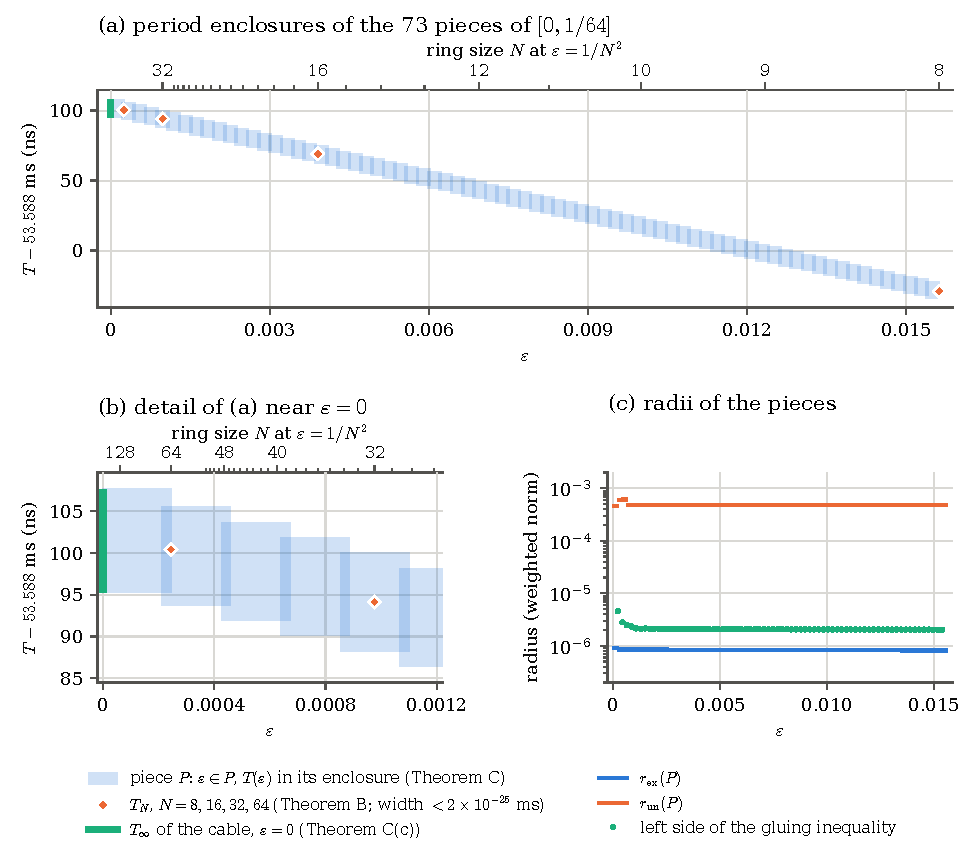
\includegraphics[width=\dimexpr\textwidth-12pt\relax]{figures/alln-pieces.pdf}
\caption{The pieces of the proof of Theorem~\ref{thm:alln}, as stored in \texttt{data/\allowbreak fourier-existence-alln.json}. (a) Each of the 73 boxes is a piece $P$ (width $1/4096$; consecutive pieces overlap by $1/32768$ and are darker where they overlap) times its period interval: for every $\varepsilon \in P$, $T(\varepsilon) = 2\pi/\omega_*(\varepsilon)$ lies in that interval. Diamonds: the periods $T_N$ of Theorem~\ref{thm:ring} at $\varepsilon = 1/N^2$, $N = 8, 16, 32, 64$ (Table~\ref{tab:existence}), whose enclosures are narrower than $2 \times 10^{-25}$~ms; each lies in the period interval of every piece that contains $1/N^2$ (Table~\ref{tab:alln}). Bar at $\varepsilon = 0$: the period $T_\infty \in [53.58809529823299300232974, 53.58810763684487454838746]$~ms of the cable wave (Theorem~\ref{thm:alln}(c)), the interval of the piece $[0, 1/4096]$. The vertical axis is $T - 53.588$~ms in ns; $53.588$~ms is an axis offset, not a result. The top axes mark $\varepsilon = 1/N^2$ at the labelled $N$, with minor ticks at the other integers $N$ up to $29$ in (a) and up to $52$ in (b); these points accumulate at $\varepsilon = 0$. (b) The part of (a) with $\varepsilon \le 5/4096$: the rings $N = 32$ and $N = 64$ ($1/4096$ lies in two pieces) and the cable. (c) For each piece, the existence radius $r_{\mathrm{ex}}(P)$ and the uniqueness radius $r_{\mathrm{un}}(P)$, drawn over the piece, both in the weighted norm $\|\cdot\|_\eta$ of that piece; and, at the middle of each of the 72 overlaps, the left side of the gluing inequality \eqref{eq:glue}, in the norm of the later piece $P_b$, which must not exceed $r_{\mathrm{un}}(b)$; its largest ratio to $r_{\mathrm{un}}(b)$ is below $0.0076$ (Section~\ref{sec:alln}). The weights differ from piece to piece, so the values in (c) are not in one common norm. The figure draws stored enclosures and radii only; stability is proved only for $N = 8$, $16$, $32$, $64$. Reproduced by \texttt{code/\allowbreak plot\_cardiac\_rings.py}.}
\label{fig:alln}
\end{figure}

\section{Stability through one Hill operator}\label{sec:stability}

\subsection{Setting}\label{sec:hill}

Let $\phi$, $\omega$, $T$, $\tau$ be as in Section~\ref{sec:ringsym}, with $\phi$ solving \eqref{eq:profile}, and let $A(\theta) = Df(\phi(\theta)) = \sum_n A_n e^{in\theta}$, a real analytic $2\pi$-periodic matrix function, so $A_{-n} = \overline{A_n}$ and $\|A_n\|$ decays exponentially. The linearization along $x(t)$ is $y' = L(t)y$ with $(L(t)y)_j = A(\theta_j(t))y_j + cE(y_{j-1} - 2y_j + y_{j+1})$; let $Y(t)$ be its fundamental matrix with $Y(0) = I$, and $M_\tau = Q^{-1}Y(\tau)$, the derivative at $x(0)$ of $h = Q^{-1}\varphi_\tau$. The Floquet multipliers are the eigenvalues of $Y(T)$, with algebraic multiplicity. For a matrix $M$ let $m(\lambda; M)$ be the algebraic multiplicity and $G_\lambda(M)$ the generalized eigenspace; for an operator $H$, $G_\mu(H) = \bigcup_k\ker(H - \mu)^k$ (with the convention of Appendix~\ref{app:resolvent} on the domains of powers of $H$) and $m(\mu; H) = \dim G_\mu(H)$.

Let $|\cdot|_1$ be the $\ell^1$ norm on $\C^{18}$, $\|B\|_{1\to1}$ the induced norm, $\Xsp = \ell^1(\Z; \C^{18})$ with $\|P\| = \sum_m|P_m|_1$, and $\Dsp = \{P \in \Xsp : \sum_m |m||P_m|_1 < \infty\}$. A sequence $P \in \Dsp$ is the coefficient sequence of the $C^1$ function $p(\theta) = \sum_m P_m e^{im\theta}$. The Hill operator $H_0: \Dsp \to \Xsp$ is
\begin{equation}\label{eq:H0}
  (H_0P)_m = -i\omega mP_m + \sum_n A_nP_{m-n} - d_mEP_m,
\end{equation}
the coefficient sequence of $\Lop p := -\omega p' + Ap + cE\Delta_Np$. The ansatz $y_j(t) = e^{\mu t}p(\theta_j(t))$ solves the linearization if and only if $\Lop p = \mu p$.

We use three standard facts about an operator $H$ with compact resolvent on $\Xsp$, or on the $\ell^1$ space of Section~\ref{sec:riesz}, which Appendix~\ref{app:resolvent} proves (Lemma~\ref{lem:A-res}(c) and Theorem~\ref{thm:A-compact}; see also Kato's book \cite[Ch.~III, Sect.~6]{kato1976}): its spectrum consists of isolated eigenvalues of finite algebraic multiplicity; for a bounded open rectangle $\Omega$ whose boundary $\Gamma$ lies in the resolvent set, the Riesz projection $\frac{1}{2\pi i}\oint_\Gamma(\mu - H)^{-1}d\mu$ ($\Gamma$ counterclockwise) is a projection onto the sum of the generalized eigenspaces of the eigenvalues in $\Omega$, so its rank is $n(H, \Omega) := \sum_{\mu\in\Omega}m(\mu; H)$; and the resolvent is holomorphic on the resolvent set.

\begin{lemma}\label{lem:H0}
$H_0$ is closed on $\Dsp$ and has compact resolvent, and $\{\re\mu > \alpha\}$ lies in its resolvent set, where $\alpha = \sum_n\|A_n\|_{1\to1} + 4c$.
\end{lemma}

\begin{proof}
Write $H_0 = D_0 + B$ with $(D_0P)_m = -i\omega mP_m$ on $\Dsp$ and $B$ the rest. By Young's inequality and $d_m \le 4c$, $\|B\| \le \alpha$. $D_0$ is closed (a diagonal operator on its maximal domain), and for $\lambda \notin i\omega\Z$, $(\lambda - D_0)^{-1}$ is diagonal with entries $(\lambda + i\omega m)^{-1}$, compact as the norm limit of its finite truncations. If $\re\lambda > \alpha$, then $\|(\lambda - D_0)^{-1}\| \le 1/\re\lambda$, so $\|B(\lambda - D_0)^{-1}\| < 1$ and $\lambda - H_0 = (I - B(\lambda - D_0)^{-1})(\lambda - D_0)$ is a bijection $\Dsp \to \Xsp$ with compact inverse. $H_0$ is closed as a closed operator plus a bounded one, and compactness of the resolvent at one point gives it everywhere by the resolvent identity $R(\lambda) = R(\lambda_0)(I + (\lambda_0 - \lambda)R(\lambda))$.
\end{proof}

\subsection{The Hill-sector theorem}\label{sec:hillsector}

\begin{lemma}[twisted periodicity]\label{lem:twist}
$L(t + \tau) = QL(t)Q^{-1}$, $Y(t + \tau) = QY(t)M_\tau$, $Y(k\tau) = Q^kM_\tau^k$ and $Y(T) = M_\tau^N$.
\end{lemma}

\begin{proof}
$(QL(t)Q^{-1}y)_j = A(\theta_{j+1}(t))y_j + cE(y_{j-1} - 2y_j + y_{j+1}) = (L(t + \tau)y)_j$, because $(Q^{-1}y)_k = y_{k-1}$ and $\theta_{j+1}(t) = \theta_j(t + \tau)$. So $Z(t) = Q^{-1}Y(t + \tau)$ solves $Z' = L(t)Z$ with $Z(0) = M_\tau$, and $Z(t) = Y(t)M_\tau$. Induction gives $Y(k\tau) = Q^kM_\tau^k$, and $Q^N = I$ gives $Y(T) = M_\tau^N$.
\end{proof}

\begin{thmx}[Hill sectors]\label{thm:hill}
For every $\mu \in \C$, $m(\mu; H_0) = m(e^{\mu\tau}; M_\tau)$.
\end{thmx}

\begin{proof}
Let $\lambda = e^{\mu\tau}$.

\emph{$m(\mu; H_0) \le m(\lambda; M_\tau)$.} Let $G = G_\mu(H_0)$, read through the Fourier correspondence as a finite-dimensional (Lemma~\ref{lem:H0} and Theorem~\ref{thm:A-compact}(iii)) $\Lop$-invariant space of $C^1$ functions, with $\Lop|_G = \mu + K_G$, $K_G$ nilpotent. For $p \in G$ put $u(t) = e^{t\Lop_G}p \in G$ and $y_j(t) = u(t)(\theta_j(t))$. The chain rule gives $y_j' = (\Lop_Gu + \omega u')(\theta_j) = (Au + cE\Delta_Nu)(\theta_j) = A(\theta_j)y_j + cE(y_{j-1} - 2y_j + y_{j+1})$, so $y$ solves the linearization with $y(0) = \iota^*p$, $\iota^*p := (p(2\pi j/N))_{j\in\Z_N}$. As $\theta_j(t + \tau) = \theta_{j+1}(t)$, $y(\tau) = Q\iota^*(e^{\tau\Lop_G}p)$; also $y(\tau) = Y(\tau)\iota^*p$. Hence $M_\tau\iota^* = \iota^*e^{\tau\Lop_G}$ on $G$. The map $\iota^*$ is injective on $G$: if $\iota^*p = 0$ then $y = 0$, so for all $t$, $j$ and integers $n$, $0 = u(t + nT)(\theta_j(t)) = e^{\mu(t+nT)}\sum_k\frac{(t+nT)^k}{k!}(K_G^kp)(\theta_j(t))$. For fixed $t, j$ this is $e^{\mu(t+nT)}$ times a polynomial in $n$ vanishing at every integer, so all its coefficients vanish; if $p \ne 0$ and $k^*$ is the largest $k$ with $K_G^kp \ne 0$, the coefficient of $n^{k^*}$ is $\frac{T^{k^*}}{k^*!}(K_G^{k^*}p)(\theta_j(t))$, so $K_G^{k^*}p$ vanishes at every point, a contradiction. So $\iota^*(G)$ is an $M_\tau$-invariant space of dimension $\dim G$ on which $M_\tau$ is similar to $\lambda e^{\tau K_G}$, whose only eigenvalue is $\lambda$; hence $\iota^*(G) \subset G_\lambda(M_\tau)$.

\emph{$m(\mu; H_0) \ge m(\lambda; M_\tau)$.} Let $W = G_\lambda(M_\tau)$, $r = \dim W \ge 1$, and on $W$ write $M_\tau = \lambda(I + K)$, $K$ nilpotent. Put $B = \mu I + \tau^{-1}\sum_{k=1}^r(-1)^{k+1}K^k/k$ on $W$. Then $e^{\tau B} = \lambda\exp(\log(I + K)) = M_\tau$ on $W$ (an identity of formal power series, valid for nilpotent $K$), $B$ commutes with $M_\tau|_W$, and the only eigenvalue of $B$ is $\mu$. Let $\Pi(t) = Y(t)e^{-tB}: W \to \C^{18N}$. By Lemma~\ref{lem:twist}, $\Pi(t + \tau)w = QY(t)M_\tau e^{-\tau B}e^{-tB}w = Q\Pi(t)w$, so $\Pi_j(t)w = \Pi_0(t + j\tau)w$ and $\Pi_0(t + T)w = \Pi_0(t)w$. Hence $p_w(\theta) := \Pi_0(\theta/\omega)w$ is $2\pi$-periodic, $C^\infty$, with coefficients in $\Dsp$, and $\Pi_j(t)w = p_w(\theta_j(t))$. Differentiating $Y(t)w = \Pi(t)e^{tB}w$ gives $L(t)\Pi(t)w = \Pi'(t)w + \Pi(t)Bw$, whose component $0$ at $t = \theta/\omega$ reads $\Lop p_w = p_{Bw}$. The map $w \mapsto p_w$ is injective ($p_w(2\pi j/N) = w_j$), so its image is an $\Lop$-invariant space of dimension $r$ on which $(\Lop - \mu)^r = 0$; it lies in $G_\mu(H_0)$.
\end{proof}

\begin{corollary}\label{cor:strip}
(i) $\spec H_0 = \{\mu : e^{\mu\tau} \in \spec M_\tau\}$, invariant with multiplicities under $\mu \mapsto \mu + i\omega N$ and $\mu \mapsto \bar\mu$.
(ii) For every real $a$, on the half-open strip $S_a = \{a \le \im\mu < a + \omega N\}$ the map $\mu \mapsto e^{\mu\tau}$ is a bijection from $\spec H_0 \cap S_a$ onto $\spec M_\tau$ preserving algebraic multiplicities, and these multiplicities add up to $18N$.
(iii) For $\rho \ne 0$, $m(\rho; Y(T)) = \sum\{m(\mu; H_0) : \mu \in \spec H_0 \cap S_a,\ e^{\mu T} = \rho\}$.
(iv) Let $H_q$ be $H_0$ with $d_m$ replaced by $d_{m+q}$. Then $H_q$ is similar to $H_0 + i\omega q$ by the shift $(\mathcal R_qP)_k = P_{k-q}$, so the ``$N$ sectors'' $H_q$, $q \in \Z_N$, carry no information beyond $H_0$.
\end{corollary}

\begin{proof}
(i) Theorem~\ref{thm:hill} in both directions (every logarithm of an eigenvalue of $M_\tau$ is an eigenvalue of $H_0$), $e^{i\omega N\tau} = 1$, and $M_\tau$ real. (ii) $e^{\mu\tau}$ has period $i\omega N$, so it is injective on $S_a$ and onto $\C\setminus\{0\}$; $M_\tau$ is invertible. (iii) $Y(T) = M_\tau^N$; $\C^{18N}$ is the sum of the $G_\lambda(M_\tau)$, each invariant under $M_\tau^N$ with only eigenvalue $\lambda^N = e^{\mu T}$. (iv) Substitute $k = m + q$.
\end{proof}

\begin{remark}[half-open strips]\label{rem:halfopen}
The count $18N$ holds in a half-open strip of height $\omega N$. A closed strip $|\im\mu| \le \omega N/2$ can count an eigenvalue twice: the logarithms of a negative real eigenvalue of $M_\tau$ lie exactly on $\im\mu \in \omega N/2 + \omega N\Z$, and since $M_\tau$ is real, a simple negative real eigenvalue stays real and negative under small real perturbations, so this is not a non-generic accident. The certificate below counts eigenvalues only inside a rectangle whose boundary lies in the resolvent set.
\end{remark}

\begin{corollary}[section maps]\label{cor:section}
Let $\mathcal S$ be a $C^1$ hypersurface through $x^* = x(0)$ transverse to $F(x^*)$, and $g(z) = Q^{-1}\varphi_{t_g(z)}(z)$ a section map with $t_g$ of class $C^1$, $t_g(x^*) = \tau$, $g(\mathcal S) \subset \mathcal S$. Then $\det(\lambda I - M_\tau) = (\lambda - 1)\det(\lambda I - Dg(x^*))$.
\end{corollary}

\begin{proof}
$Y(\tau)F(x^*) = F(x(\tau)) = QF(x^*)$, so $M_\tau F(x^*) = F(x^*)$. $Dg(x^*) = M_\tau + F(x^*)Dt_g(x^*)$ on $T\mathcal S$ maps $T\mathcal S$ into itself, so it is the compression of $M_\tau$ along $F(x^*)$; in the splitting $\operatorname{span}F(x^*) \oplus T\mathcal S$, $M_\tau$ is block upper triangular with diagonal blocks $1$ and $Dg(x^*)$.
\end{proof}

\subsection{The trivial multiplier}\label{sec:trivial}

\begin{lemma}\label{lem:trivial}
(a) $P^* = (ima_m)_m$, the coefficients of $\phi'$, is a nonzero element of $\Dsp$ with $H_0P^* = 0$. (b) $m(1; Y(T)) = \sum_{q=0}^{N-1}m(i\omega q; H_0)$. (c) The multiplier $1$ is algebraically simple if and only if $m(0; H_0) = 1$ and $i\omega q \notin \spec H_0$ for $q = 1, \dots, N - 1$.
\end{lemma}

\begin{proof}
(a) $\phi$ is analytic and nonconstant; differentiating \eqref{eq:profile} gives $\Lop\phi' = 0$. (b) Corollary~\ref{cor:strip}(iii) with $\rho = 1$, $a = -\omega/2$: $e^{\mu T} = 1$ iff $\mu \in i\omega\Z$, and $i\omega q \in S_{-\omega/2}$ iff $q = 0, \dots, N-1$. (c) follows from (a) and (b).
\end{proof}

An eigenvalue $i\omega q$, $q \not\equiv 0 \pmod N$, would be a neutral mode of the reduced map (a spatial phase twist) that merges with the multiplier $1$ of $Y(T)$. The certificate below excludes it together with everything else in $\{\re\mu \ge -\delta\}$.

\subsection{Exclusion and counting by a Riesz-projection homotopy}\label{sec:riesz}

Goal: for a given $\delta > 0$, prove
\begin{equation}\label{eq:G}
  \spec H_0 \cap \{\re\mu \ge -\delta\} = i\omega N\Z, \quad\text{each eigenvalue algebraically simple.}
\end{equation}

\begin{lemma}\label{lem:projrank}
If $P$, $P'$ are bounded projections on a Banach space, $\|P - P'\| < 1$ and $\rank P < \infty$, then $\rank P' = \rank P$.
\end{lemma}

\begin{proof}
If $x \in \Ran P'$ and $Px = 0$ then $\|x\| = \|(P' - P)x\| < \|x\|$ unless $x = 0$; so $P$ maps $\Ran P'$ injectively into $\Ran P$. Exchange the roles.
\end{proof}

\begin{lemma}[homotopy count]\label{lem:homotopy}
Let $X$ be one of the spaces $\ell^1_w(\mathcal J)$ of Appendix~\ref{app:resolvent}, $\hat D$ an operator in $X$ with compact resolvent, $\hat E \in B(X)$, $\Omega$ a bounded open rectangle whose boundary $\Gamma$ lies in the resolvent set of $\hat D$, and suppose $I - s\hat E(\mu - \hat D)^{-1}$ is invertible for all $(s, \mu) \in [0,1] \times \Gamma$. Then, with $H(s) = \hat D + s\hat E$, $\Gamma$ lies in the resolvent set of every $H(s)$ and $n(H(1), \Omega) = n(\hat D, \Omega)$.
\end{lemma}

\begin{proof}
This is Theorem~\ref{thm:A-homotopy}.
\end{proof}

\paragraph{The comparison operator.} The program fixes:
\begin{itemize}
\item cell coordinates: an exact diagonal $S = \operatorname{diag}(2^{k_1}, \dots, 2^{k_{18}})$, applied in every mode (its exponents $k_l$ are chosen per $N$ and stored in the records; they are not the scale exponents $e_i$ of Section~\ref{sec:cell}). This is a similarity; it commutes with $E$, leaves $-i\omega m$ and $d_m$ unchanged, and changes no spectrum or multiplicity. From here on $A_n$ and every norm are taken in these coordinates;
\item a window $W = \{|m| \le K_e\}$ ($n_W = 18(2K_e + 1)$ coordinates) and the tail $\mathrm{Tl} = \{|m| > K_e\}$;
\item a complex $n_W \times n_W$ matrix $V$ with exactly representable entries (its invertibility is checked in (C3)) and a diagonal $\Lambda = \operatorname{diag}(\lambda_j)$ with exactly representable entries (floating-point eigenvectors and eigenvalues of the window block);
\item an exact real $18 \times 18$ matrix $A_0^c$ (the midpoint of the enclosure of $A_0$), and for each residue $r \in \{0, \dots, \lfloor N/2\rfloor\}$ a complex $18 \times 18$ matrix $U_r$ with exactly representable entries (its invertibility is checked in (C2)) and an exact diagonal $\Lambda_r$ approximately diagonalizing $X_r := A_0^c - d_rE$;
\item the rectangle $\Omega = (-\delta, R_0) \times (a, b)$ (real part, imaginary part), with boundary $\Gamma$.
\end{itemize}
Let $\mathrm{Scal}$ be $V$ on the window coordinates and the identity on the tail; it is bounded, boundedly invertible and maps $\Dsp$ onto $\Dsp$. Define
\[ \hat D = \Lambda \oplus \bigoplus_{m\in\mathrm{Tl}}B_m, \qquad B_m = -i\omega mI + X_{m \bmod N}, \qquad \hat E = \mathrm{Scal}^{-1}H_0\,\mathrm{Scal} - \hat D. \]
The domain of $\hat D$ is $D(\hat D) = \{v : \sum_{m\in\mathrm{Tl}}|m||v_m|_1 < \infty\}$, the window coordinates being unrestricted; it is the maximal domain of the block-diagonal $\hat D$, because $(\omega|m| - \|X_r\|_{1\to1})|v_m|_1 \le |B_mv_m|_1 \le (\omega|m| + \|X_r\|_{1\to1})|v_m|_1$ with $r = m \bmod N$. Since $\mathrm{Scal}$ acts only on the finitely many window coordinates, $\mathrm{Scal}^{-1}(\Dsp) = D(\hat D)$. In blocks, $\hat E_{WW} = R_W := V^{-1}H_{WW}V - \Lambda$, $\hat E_{WT} = V^{-1}H_{WT}$, $\hat E_{TW} = H_{TW}V$ and $(\hat E_{TT}P)_m = \sum_{n \ne 0,\,m-n\in\mathrm{Tl}}A_nP_{m-n} + (A_0 - A_0^c)P_m$, where $H_{WW}$, $H_{WT}$, $H_{TW}$ are the blocks of $H_0$; in the tail diagonal the damping $-d_mE$ of $H_0$ cancels exactly against the $-d_{m \bmod N}E$ in $X_{m \bmod N}$, by \eqref{eq:damping}, and $-i\omega m$ cancels against $B_m$. These formulas define $\hat E$ as a bounded operator on the whole space ($R_W$ is a finite matrix, and the other blocks have column sums bounded by $\sum_n\|A_n\|_{1\to1}$ times constants), and on $D(\hat D)$ it equals $\mathrm{Scal}^{-1}H_0\,\mathrm{Scal} - \hat D$; so $\hat D + \hat E = \mathrm{Scal}^{-1}H_0\,\mathrm{Scal}$ as operators with the same domain $D(\hat D)$. The exact $\omega$ stays in $B_m$: an error $(\omega - \bar\omega)m$ is unbounded in $m$ and cannot be moved into $\hat E$. The norm on the $\mathrm{Scal}$-coordinates $v$ is $\|v\| = \sum_j|v_j| + \sum_{m\in\mathrm{Tl}}|v_m|_1$ (all weights equal to $1$ in the runs), and the norm of an operator is the supremum of its column sums.

\paragraph{Notation for the bounds.} All are upper bounds unless compared from below:
\begin{itemize}
\item $\operatorname{dist}_j$: the distance from $\lambda_j$ to $\Gamma$ (a lower bound);
\item $f\!m_j$: the $\ell^1$ norm of column $j$ of $R_W$; $r_j = \sum_{w\in W}t_w|V_{(w,\cdot),j}|_1$ with $t_w = \sum_{|w+n| > K_e}\|A_n\|_{1\to1}$;
\item $b_m = \max_k\sum_j|(V^{-1}H_{W,m})_{j,k}|$ for $m \in \mathrm{Tl}$, where $H_{W,m}$ has entries $(A_{w-m})_{l,k}$ in row $(w, l)$; $\hat b = \sup_{m\in\mathrm{Tl}}b_m$;
\item $\sigma_{\mathrm{off}} = \sum_{n\ne0}\|A_n\|_{1\to1}$ and $\theta_c = \sigma_{\mathrm{off}} + \|A_0 - A_0^c\|_{1\to1}$;
\item $\rho_T$: a bound of $\|(\mu - B_m)^{-1}\|_{1\to1}$ over $\mu \in \overline\Omega$ and $m \in \mathrm{Tl}$ (Lemma~\ref{lem:tail}), and $\theta_T = \theta_c\rho_T$.
\end{itemize}

\begin{lemma}[tail blocks]\label{lem:tail}
Let $h = \max(|a|, |b|)$, $\omega_{\mathrm{lo}} \le \omega$, $g_0 = \omega_{\mathrm{lo}}(K_e + 1) - h$, $\eta > 0$, and
\[ \gamma_r = \min_l\max\big(-\delta - \eta - \re\lambda_{r,l},\ g_0 - \eta - |\im\lambda_{r,l}|\big), \quad F_r = U_r^{-1}X_rU_r - \Lambda_r, \quad \kappa_r \ge \|U_r\|_{1\to1}\|U_r^{-1}\|_{1\to1}. \]
If $\gamma_r > \|F_r\|_{1\to1}$ for every $r$, then for every $\mu$ in the open neighborhood $N_\eta = \{-\delta - \eta < \re\mu < R_0 + \eta,\ |\im\mu| < h + \eta\}$ of $\overline\Omega$ and every $m \in \mathrm{Tl}$, $\mu - B_m$ is invertible with $\|(\mu - B_m)^{-1}\|_{1\to1} \le \rho_T := \max_r\kappa_r/(\gamma_r - \|F_r\|_{1\to1})$. Moreover, for fixed $\mu$, $\|(\mu - B_m)^{-1}\|_{1\to1} \to 0$ as $|m| \to \infty$.
\end{lemma}

\begin{proof}
$\mu - B_m = z - X_r$ with $z = \mu + i\omega m$ and $r = m \bmod N$ (or $N - r$, which gives the same $X_r$). For $m \ge K_e + 1$, $\re z = \re\mu > -\delta - \eta$ and $\im z \ge \omega_{\mathrm{lo}}(K_e + 1) - h - \eta = g_0 - \eta$; for $m \le -(K_e + 1)$ the same holds for $\bar z$, and since $X_r$ is real, $(\bar z - X_r)^{-1} = \overline{(z - X_r)^{-1}}$ has the same norm. For such $z$, $|z - \lambda_{r,l}| \ge \max(-\delta - \eta - \re\lambda_{r,l}, g_0 - \eta - |\im\lambda_{r,l}|) \ge \gamma_r$, so $\|(z - \Lambda_r)^{-1}\| \le 1/\gamma_r$, and $z - X_r = U_r(z - \Lambda_r - F_r)U_r^{-1}$ with the Neumann series gives the bound. The decay follows from the Neumann bound $1/(|\mu + i\omega m| - \|X_r\|)$.
\end{proof}

\begin{lemma}[comparison operator]\label{lem:compare}
If the hypothesis of Lemma~\ref{lem:tail} holds and $\operatorname{dist}_j > 0$ for every $j$, then $\hat D$ has compact resolvent, $\Gamma$ lies in its resolvent set, $n(\hat D, \Omega) = \#\{j : \lambda_j \in \Omega\}$, and $\|(\mu - \hat D)^{-1}\| \le \max(\max_j 1/\operatorname{dist}_j, \rho_T)$ on $\Gamma$.
\end{lemma}

\begin{proof}
$\hat D$ is block diagonal. Let $D_T$ be the tail part, with domain $D(D_T) = \{v : \sum_{m\in\mathrm{Tl}}|m||v_m|_1 < \infty\}$ in the tail space. For $\mu \in N_\eta$, Lemma~\ref{lem:tail} gives $\|(\mu - B_m)^{-1}\|_{1\to1} \le \rho_T$ for every $m \in \mathrm{Tl}$, and $B_m(\mu - B_m)^{-1} = \mu(\mu - B_m)^{-1} - I$ has norm at most $1 + |\mu|\rho_T$. So the block-diagonal operator with blocks $(\mu - B_m)^{-1}$ maps the tail space into $D(D_T)$ (by the lower bound on $|B_mv_m|_1$ above), it is inverse to $\mu - D_T$ on both sides, and its norm, the supremum of the $1\to1$ norms of its blocks, is at most $\rho_T$: $\mu - D_T$ is a bijection of $D(D_T)$ onto the tail space with inverse of norm at most $\rho_T$. For fixed $\mu$ the blocks of the inverse tend to $0$ in norm, so its finite truncations converge to it in norm, and it is compact. The resolvent of $D_T$ is holomorphic on $N_\eta \supset \overline\Omega$, so its contour integral over $\Gamma$ vanishes (Lemmas~\ref{lem:A-res}(c) and~\ref{lem:A-int}(d)), and the Riesz projection of $\hat D$ for $\Omega$ is the diagonal projection onto the window coordinates with $\lambda_j \in \Omega$; its rank is $n(\hat D, \Omega)$ by Theorem~\ref{thm:A-compact}(iv).
\end{proof}

\begin{lemma}[small gain, Schur-complement form]\label{lem:smallgain}
Under the hypotheses of Lemma~\ref{lem:compare}, if $\theta_T < 1$, $\hat b < \infty$ and
\begin{equation}\label{eq:SC}
  f\!m_j + \frac{\hat b\,\rho_T\,r_j}{1 - \theta_T} < \operatorname{dist}_j \qquad\text{for every window column } j, \tag{SC}
\end{equation}
then $I - s\hat E(\mu - \hat D)^{-1}$ is invertible for every $(s, \mu) \in [0,1] \times \Gamma$.
\end{lemma}

\begin{proof}
Fix $(s, \mu)$. The tail block of $\mu - \hat D - s\hat E$ is $(I - s\hat E_{TT}(\mu - D_T)^{-1})(\mu - D_T)$, invertible with $\|(\mu - D_T - s\hat E_{TT})^{-1}\| \le \rho_T/(1 - \theta_T)$, since $\|\hat E_{TT}(\mu - D_T)^{-1}\| \le \theta_c\rho_T$ (the column sums of $\hat E_{TT}$ are at most $\sum_{n\ne0}\|A_n\| + \|A_0 - A_0^c\|$). By the block factorization (valid because the window block is finite-dimensional and both triangular factors are bijections of the domain), $\mu - \hat D - s\hat E$ is invertible if and only if the Schur complement
\[ \mathrm{Sc} = \mu - \Lambda - sR_W - s^2\hat E_{WT}(\mu - D_T - s\hat E_{TT})^{-1}\hat E_{TW} = (I - C_c(\mu - \Lambda)^{-1})(\mu - \Lambda) \]
is invertible, with $C_c = sR_W + s^2\hat E_{WT}(\cdots)^{-1}\hat E_{TW}$. Column $j$ of $\hat E_{TW}$ has norm at most $r_j$ (its tail rows are $\sum_w A_{m-w}V_{(w,\cdot),j}$, and $\sum_{m\in\mathrm{Tl}}\|A_{m-w}\| \le t_w$), and $\|\hat E_{WT}u\| \le \sum_{m,k}|u_{m,k}|b_m \le \hat b\|u\|$. So column $j$ of $C_c$ has norm at most $f\!m_j + \hat b\rho_Tr_j/(1 - \theta_T)$, and $\|C_c(\mu - \Lambda)^{-1}\| \le \max_j(f\!m_j + \hat b\rho_Tr_j/(1 - \theta_T))/\operatorname{dist}_j < 1$. Then $\mu - \hat D - s\hat E$ is invertible, which is equivalent to the claim because $\mu - \hat D$ is.
\end{proof}

The condition \eqref{eq:SC} asks only for the product of the window-to-tail coupling $\hat b$ and the tail-to-window coupling $r_j$ of each column to be small, which suits the problem: eigenvectors of near-axis eigenvalues are small at the window edge. The programs also evaluate the stronger form in which the window and tail columns are bounded separately; it does not hold at any $N$ and is not used.

\begin{lemma}[coupling sums from coefficient bounds]\label{lem:coupling}
Suppose enclosures $[A_n]$ of $A_n$ are known for $|n| \le n_A$ and $\|A_n\|_{1\to1} \le s_1q_1^{|n|} + s_2q_2^{|n|}$ for every $n$ ($q_1, q_2 < 1$). Let $G_{\mathrm{tail}}(k) = 2\sum_i s_iq_i^k/(1 - q_i)$. Then $\sigma_{\mathrm{off}} \le \sum_{0<|n|\le n_A}\|[A_n]\| + G_{\mathrm{tail}}(n_A + 1)$; $t_w \le \sum_{|n|\le n_A,\,|w+n|>K_e}\|[A_n]\| + G_{\mathrm{tail}}(n_A + 1)$; let $n_c \ge 1$ be an integer, and let $\beta_{(w,l)} \ge \sum_j|(V^{-1})_{j,(w,l)}|$ be upper bounds of the column sums of $V^{-1}$ (for example those of Lemma~\ref{lem:Vinv}), with $\beta_{\max} = \max_{(w,l)}\beta_{(w,l)}$. For every $m$ in the tail, $b_m \le \max_k\sum_{(w,l)}\beta_{(w,l)}|(A_{w-m})_{l,k}|$. For $K_e < |m| \le K_e + n_c$, the right side is bounded from the entrywise enclosures $[A_{w-m}]$ (for $|w - m| > n_A$, the entrywise tail enclosures of Section~\ref{sec:coeffs}). For $|m| > K_e + n_c$, $b_m \le \beta_{\max}G_{\mathrm{tail}}(|m| - K_e)/2$, a bound that decreases in $|m|$.
\end{lemma}

\begin{proof}
Sums of upper bounds, with exact geometric sums. The first bound on $b_m$ is the triangle inequality applied to $(V^{-1}H_{W,m})_{j,k} = \sum_{(w,l)}(V^{-1})_{j,(w,l)}(A_{w-m})_{l,k}$, summed over $j$. For the last bound,
\[
\sum_{(w,l)}\beta_{(w,l)}|(A_{w-m})_{l,k}| \le \beta_{\max}\sum_w\|A_{w-m}\|_{1\to1},
\]
and the indices $n = w - m$ have one sign with $|n| \ge |m| - K_e$.
\end{proof}

\begin{lemma}[the window without inverting $V$]\label{lem:Vinv}
Let $V_i$ be an exact floating-point approximate inverse of $V$, $C = I - V_iV$, and suppose $q_C := \|C\| < 1$. Then $V$ is invertible, $V^{-1} = (I - C)^{-1}V_i$ with $\|(I - C)^{-1}\| \le 1/(1 - q_C)$, and with $\Xi := V_iH_{WW}V - \Lambda$,
\[ f\!m_j \le \frac{\|\Xi e_j\| + |\lambda_j|\,\|Ce_j\|}{1 - q_C}, \qquad \sum_j|(V^{-1})_{j,(w,l)}| \le \frac{\|V_ie_{(w,l)}\|}{1 - q_C}. \]
\end{lemma}

\begin{proof}
$V_iV = I - C$ is invertible by the Neumann series, so $V$ is invertible and $V^{-1} = (V_iV)^{-1}V_i$. Since $V_iV\Lambda = \Lambda - C\Lambda$, $V_i(H_{WW}V - V\Lambda) = \Xi + C\Lambda$ exactly, so $R_W = V^{-1}(H_{WW}V - V\Lambda) = (I - C)^{-1}(\Xi + C\Lambda)$, and $C\Lambda e_j = \lambda_jCe_j$.
\end{proof}

\begin{thmx}[the certificate]\label{thm:cert}
Suppose the following are checked in ball arithmetic:
\begin{enumerate}
\item[(C0)] $\omega \in [\omega_{\mathrm{lo}}, \omega_{\mathrm{hi}}]$, $\omega_{\mathrm{lo}} > 0$; entrywise enclosures $[A_n]$ of the true $A_n$ for every $n$ that enters (those of Section~\ref{sec:coeffs}, for $|n| \le n_A$ and beyond) and the tail form of Lemma~\ref{lem:coupling}; balls containing $d_m$;
\item[(C1)] $\delta > 0$; $R_0 > \alpha^{\mathrm{up}} \ge \alpha$; $a < 0 < b$, $b - a \ge \omega_{\mathrm{hi}}N$, $b < \omega_{\mathrm{lo}}N$, $-a < \omega_{\mathrm{lo}}N$;
\item[(C2)] the hypothesis of Lemma~\ref{lem:tail} for $r = 0, \dots, \lfloor N/2\rfloor$, with $U_r$ certified invertible by Arb inversion of the exact matrix $U_r$, and with the norms of $U_r^{-1}$ that the lemma uses bounded from that enclosure;
\item[(C3)] $V$ invertible and $f\!m_j$ bounded from a ball matrix containing the true $H_{WW}$ (with the ball $[\omega_{\mathrm{lo}}, \omega_{\mathrm{hi}}]$ on its diagonal); $\operatorname{dist}_j > 0$ for every $j$;
\item[(C4)] $\theta_T < 1$ and \eqref{eq:SC};
\item[(C5)] exactly one $\lambda_j$ lies in $\Omega$.
\end{enumerate}
Then \eqref{eq:G} holds.
\end{thmx}

\begin{proof}
By Lemmas~\ref{lem:compare} and~\ref{lem:smallgain}, Lemma~\ref{lem:homotopy} applies to $\hat D$ and $\hat E$, so $n(\mathrm{Scal}^{-1}H_0\mathrm{Scal}, \Omega) = n(\hat D, \Omega) = 1$ and $\Gamma$ lies in the resolvent set of $H_0$; the similarity by $\mathrm{Scal}$ gives $n(H_0, \Omega) = 1$. By (C1), $0 \in \Omega$, and $0$ is an eigenvalue (Lemma~\ref{lem:trivial}(a)), so it is the only eigenvalue in $\Omega$ and $m(0; H_0) = 1$. Let $\mu$ be an eigenvalue with $\re\mu \ge -\delta$. By Lemma~\ref{lem:H0}, $\re\mu \le \alpha < R_0$. Since $b - a \ge \omega_{\mathrm{hi}}N \ge \omega N$, some $\mu' = \mu + i\omega Nk$ has $a \le \im\mu' < a + \omega N \le b$, and $\mu'$ is an eigenvalue of the same multiplicity (Corollary~\ref{cor:strip}(i)). As $\Gamma$ is in the resolvent set, $\mu' \in \Omega$, so $\mu' = 0$, $\mu \in i\omega N\Z$ and $m(\mu; H_0) = 1$.
\end{proof}

The conditions $b < \omega_{\mathrm{lo}}N$ and $-a < \omega_{\mathrm{lo}}N$ are not needed for soundness (if $\Omega$ contained $\pm i\omega N$, the certificate could not pass, since by Theorem~\ref{thm:cert}'s argument $\Omega$ would contain at least two eigenvalues of $H_0$); they are needed for a correct spectrum to pass.

\subsection{From the existence ball to the coefficients}\label{sec:coeffs}

Theorem~\ref{thm:cert} needs enclosures of the coefficients $A_n$ of $Df(\phi_*(\theta))$ for the true profile, which is known only to lie in the ball of Theorem~\ref{thm:ring}(a). Let $J_n$ be the coefficients of $Df(\phi_{\bar a}(\theta))$ for the center, enclosed as in Section~\ref{sec:fe} with the entrywise strip bound $|J_{n,kl}| \le S_{J,kl}e^{-\rho|n|}$, and let $M_k$ and $R_j$ be as in Section~\ref{sec:Z2}.

\begin{lemma}\label{lem:coeffs}
Let $r = r_{\mathrm{ex}}$, $\rho_e = \min(1/4, \rho_2) = 1/4$, $t_j = r$, assume $t_j < R_j$ for every $j$, and let
\[ \varepsilon_{kl} = \frac{M_k}{R_l}\Big[\Big(1 - \frac{t_l}{R_l}\Big)^{-1}\prod_j\Big(1 - \frac{t_j}{R_j}\Big)^{-1} - 1\Big]. \]
Then $|A_{kl}(\theta) - J_{kl}(\theta)| \le \varepsilon_{kl}$ for $|\im\theta| \le \rho_e$, and $|(A_n - J_n)_{kl}| \le \varepsilon_{kl}e^{-\rho_e|n|}$ for every $n$.
\end{lemma}

\begin{proof}
For $|\im\theta| \le 1/4$, $|\phi_{*,j}(\theta) - \phi_{\bar a,j}(\theta)| \le \|a_{*,j} - \bar a_j\|_\nu \le t_j$, so $w = \phi_* - \phi_{\bar a}$ lies in the polydisc of radii $t$. On the polydisc of radii $R$, $f_k(\phi_{\bar a}(\theta) + w) = \sum_\alpha c_\alpha w^\alpha$ with $|c_\alpha| \le M_kR^{-\alpha}$, so $\partial_lf_k(\phi_{\bar a} + w) - \partial_lf_k(\phi_{\bar a}) = \sum_{\alpha_l\ge1,|\alpha|\ge2}\alpha_lc_\alpha w^{\alpha - e_l}$ is bounded by the same sum for the majorant $M_k\prod_j(1 - t_j/R_j)^{-1}$, which is $\varepsilon_{kl}$. $A - J$ is holomorphic and $2\pi$-periodic on $|\im\theta| < 1/4$; Lemma~\ref{lem:cauchy} on every strip $|\im\theta| \le \rho''$, $\rho'' < 1/4$, and the limit $\rho'' \to 1/4$ give the coefficient bound.
\end{proof}

In the cell coordinates $S$ every bound transforms exactly ($(S^{-1}MS)_{kl} = M_{kl}2^{k_l - k_k}$), and from here on $[J_n]$, $S_J$ and $\varepsilon$ denote the transformed bounds. The radius must be $r_{\mathrm{ex}}$, not $r_{\mathrm{un}}$: at $N = 8$ the record gives $\|\varepsilon\|_{1\to1} \le 1.21 \times 10^{-12}$ in the coordinates $S$ with $r_{\mathrm{ex}}$; since $\varepsilon$ grows linearly in $r$ for small $r$, the radius $r_{\mathrm{un}} = 10^{-12}$ would give about $7 \times 10^3$ in the same coordinates, far above the near-axis margins $\operatorname{dist}_j \approx 1.3 \times 10^{-6}$. So the program uses the entrywise enclosures $[A_n] = [J_n] + \operatorname{ball}(0, \varepsilon e^{-\rho_e|n|})$ for $|n| \le n_A = 80$ and $[A_n] = \operatorname{ball}(0, S_Je^{-\rho|n|} + \varepsilon e^{-\rho_e|n|})$ for $|n| > 80$ (entrywise; this holds for every $n$ by Lemma~\ref{lem:cauchy} applied to $J$ on the strip $|\im\theta| \le \rho$ and by Lemma~\ref{lem:coeffs}), which is needed in the window ($|n| \le 2K_e$, up to $96$ at $N = 64$) and for $b_m$ ($|n| \le 2K_e + n_c$, up to $120$), together with the tail form $\|A_n\|_{1\to1} \le \|S_J\|e^{-\rho|n|} + \|\varepsilon\|e^{-\rho_e|n|}$ for every $n$, which is the form of Lemma~\ref{lem:coupling}.

\subsection{Conclusion for the wave}\label{sec:conclusion}

\begin{thmx}\label{thm:stab}
Assume the existence statement of Lemma~\ref{lem:real} and the certificate of Theorem~\ref{thm:cert} for some $\delta > 0$, with inputs (C0) built as in Section~\ref{sec:coeffs}. Then:
\begin{enumerate}
\item[(i)] $Y(T)$ has the eigenvalue $1$ algebraically simple, and the other $18N - 1$ Floquet multipliers satisfy $|\rho| < e^{-\delta T} \le e^{-\delta T_{\mathrm{lo}}}$, $T_{\mathrm{lo}} = 2\pi/\omega_{\mathrm{hi}}$;
\item[(ii)] $M_\tau$ has the eigenvalue $1$ algebraically simple and all others of modulus less than $e^{-\delta\tau}$, and so has every section map of Corollary~\ref{cor:section}, without the eigenvalue $1$;
\item[(iii)] the orbit is locally exponentially orbitally stable with asymptotic phase, as stated in Theorem~\ref{thm:ring}(c).
\end{enumerate}
\end{thmx}

\begin{proof}
(i) By Corollary~\ref{cor:strip}(iii) with $a = -\omega/2$, the multipliers are $e^{\mu T}$, $\mu \in \spec H_0 \cap S_a$, with multiplicities. By \eqref{eq:G}, $\mu = 0$ is simple and is the only element of $i\omega\Z \cap S_a$ in the spectrum, and every other $\mu$ has $\re\mu < -\delta$, so $|e^{\mu T}| < e^{-\delta T}$. Lemma~\ref{lem:trivial}(b) gives simplicity of the multiplier $1$. (ii) Corollaries~\ref{cor:strip}(ii) and~\ref{cor:section}.

(iii) $F$ is analytic near $O = \{x(t)\}$. Let $\mathcal S_0 = \{z : \langle F(x^*), z - x^*\rangle = 0\}$. Since $\frac{d}{dt}\langle F(x^*), \varphi_t(z) - x^*\rangle$ at $(T, x^*)$ equals $|F(x^*)|^2 > 0$, the implicit function theorem gives a neighborhood $U$ of $x^*$ and a $C^1$ function $t_S$ on $U$ with $t_S(x^*) = T$ and $\varphi_{t_S(z)}(z) \in \mathcal S_0$. The Poincar\'e map $P(z) = \varphi_{t_S(z)}(z)$ on $\mathcal S_0 \cap U$ has $P(x^*) = x^*$ and, as in Corollary~\ref{cor:section} with $Q$ replaced by $I$ and $\tau$ by $T$, $DP(x^*)$ is the compression of $Y(T)$, with spectrum that of $Y(T)$ minus one copy of $1$; by (i) its spectral radius $\varrho$ is less than $e^{-\delta T}$. Let $\delta' < \delta$, $\kappa = e^{-\delta'T}$, and choose $\kappa'$ with $\varrho < \kappa' < \kappa$. With a Jordan form $J_P = U_0^{-1}DP(x^*)U_0$ and $D_\epsilon = \operatorname{diag}(1, \epsilon_J, \epsilon_J^2, \dots)$, the norm $|v|_* = |D_\epsilon^{-1}U_0^{-1}v|_\infty$ with $0 < \epsilon_J \le \kappa' - \varrho$ gives $\|DP(x^*)\|_* \le \kappa'$. By continuity there is $\epsilon_1 > 0$ with $\|DP(z)\|_* \le \kappa$ on the ball $B_c = \{z \in \mathcal S_0 : |z - x^*|_* \le \epsilon_1\}$, which is convex; the mean value inequality gives $|P(z) - x^*|_* \le \kappa|z - x^*|_*$ there, so $P$ maps $B_c$ into itself and $|P^k(z) - x^*|_* \le \kappa^k|z - x^*|_*$.

Let $x^0$ be given and choose $s \in [0, T)$ with $|x^0 - x(s)| = \operatorname{dist}(x^0, O)$ (it exists because $O$ is compact), and $z_0 = \varphi_{T-s}(x^0)$; by Gronwall $|z_0 - x^*| \le e^{\mathrm{Lip}\,T}|x^0 - x(s)|$, so the solution meets $\mathcal S_0$ at time $t_1 = T - s + t_S(z_0) \le 3T$ at $z_1 = \varphi_{t_S(z_0)}(z_0)$ with $|z_1 - x^*| \le C_1\operatorname{dist}(x^0, O)$, and we take $\epsilon_0$ so small that $z_1 \in B_c$. Let $z_k = P^{k-1}(z_1)$ and $t_{k+1} = t_k + t_S(z_k)$. Since $|t_S(z_k) - T| \le C_2\kappa^k|z_1 - x^*|$, the limit $\sigma_\infty = \lim(t_k - kT)$ exists with $|t_k - kT - \sigma_\infty| \le C_3\kappa^k|z_1 - x^*|$. Put $\sigma = -\sigma_\infty$. For $t \in [t_k, t_{k+1}]$, $\varphi_t(x^0) = \varphi_{t-t_k}(z_k)$ and $x(t + \sigma) = \varphi_{t-t_k}(x(t_k + \sigma))$, where $x(t_k + \sigma) = x(t_k - kT - \sigma_\infty)$ lies within $\sup|F|\,C_3\kappa^k|z_1 - x^*|$ of $x^*$ and $|z_k - x^*| \le C_4\kappa^k|z_1 - x^*|$; Gronwall over an interval of length at most $2T$ gives $|\varphi_t(x^0) - x(t + \sigma)| \le C_5\kappa^k|z_1 - x^*|$, and $t \le (k+1)T + C_6$ gives $\kappa^k \le C_7e^{-\delta't}$. On $[0, t_1]$, Gronwall gives $|\varphi_t(x^0) - x(t + s)| \le e^{\mathrm{Lip}\,t}|x^0 - x(s)|$, and since $|\sigma_\infty - (t_1 - T)| \le \sum_{k\ge1}|t_S(z_k) - T| \le C'|z_1 - x^*|$ and $t_1 - T = -s + t_S(z_0)$ with $|t_S(z_0) - T| \le C|z_0 - x^*|$, $\sigma = s - T + O(\operatorname{dist}(x^0, O))$, so by $T$-periodicity $|x(t + \sigma) - x(t + s)| \le C''\operatorname{dist}(x^0, O)$. Together, on $[0, t_1]$ the difference is at most $C_8e^{3\delta'T}e^{-\delta't}\operatorname{dist}(x^0, O)$.
\end{proof}

This is the classical Andronov--Witt statement, proved here from the Poincar\'e map so that no textbook hypothesis needs matching. If $T$ were not the minimal period of the ring solution, (i) to (iii) would still hold with respect to $T$; Lemma~\ref{lem:real} shows that it is minimal.

\subsection{The computations}\label{sec:stabcomp}

The program \file{code/fourier/stability.py} implements Theorem~\ref{thm:cert} with Lemma~\ref{lem:tail} for (C2), Lemma~\ref{lem:smallgain} for (C4) and Lemma~\ref{lem:Vinv} for (C3), at 128 bits everywhere. It reads $\omega_{\mathrm{lo}}$, $\omega_{\mathrm{hi}}$, $r_{\mathrm{ex}}$ and the settings from the Stage~E record (it refuses to run if any source hash in that record differs from the current file, and it stores the SHA-256 of the record it read), and recomputes $[J_n]$, $S_J$ and $M_k$ by the same calls as the existence program; as a consistency check their suprema and the digests of the trigonometric polynomials must equal the values in the Stage~E record. It asserts $t_j < R_j$; rounds $\delta$ up to a dyadic with denominator $2^{60}$; takes $R_0 = 32$, the least power of two above $\alpha^{\mathrm{up}}$, which lies between $17.84$ and $18.11$ for the five values of $N$; takes $b = -a$ an exact double near $\bar\omega(N/2 + 1/4)$, which puts both horizontal edges a quarter of $\omega$ from the rows $\im\mu \approx \omega k$ where the near-axis eigenvalues lie; takes $K_e = \lfloor N/2\rfloor + 16$, $n_c = 24$, $\eta = 2^{-20}$; uses Lemma~\ref{lem:tail} for the tail (the program calls this ``route A''; an alternative ``route B'', a direct cover of the bounded part described in \file{code/fourier/LEMMAS-stability.md}, is not used); chooses the exponents of $S$ in floating point to make the tail bound small; computes $V$ and $\Lambda$ by LAPACK on the midpoint of the window block in the coordinates $S$, single-threaded; and decides (C1) to (C4) in Arb, where $\operatorname{dist}_j$ is an Arb lower bound of a distance computed exactly in rational arithmetic; the count (C5) is decided by exact rational comparisons of the doubles $\lambda_j$ with the dyadic edges $-\delta$, $R_0$, $a$, $b$. Floating point only chooses exact numbers, which decides whether the inequalities hold, never whether a passed inequality is true. Before any conclusion the program also checks that the residual of the trivial eigenvector $P^*$ under the window block is small (below $7 \times 10^{-17}$ in every record: about $6.6 \times 10^{-17}$ for the cell and below $3 \times 10^{-20}$ for the rings), which would expose a dropped coefficient or a wrong sign convention.

\begin{proof}[Proof of Theorem~\ref{thm:ring}(c) and Theorem~\ref{thm:cell}(ii)]
For each $N \in \{1, 8, 16, 32, 64\}$ the records \file{data/fourier-stability-N*.json} show (C0) to (C5) passed, with Lemma~\ref{lem:tail} for the tail and the form (SC): for example at $N = 8$, $\rho_T \le 3.5781$, $\theta_c \le 0.07873$, $\theta_T \le 0.2817$, $\hat b \le 0.856$, $q_C \le 2.7 \times 10^{-14}$, the smallest $\operatorname{dist}_j$ is $1.32 \times 10^{-6}$, and exactly one $\lambda_j$ (at about $3 \times 10^{-16} - 4 \times 10^{-15}i$) lies in $\Omega$; Table~\ref{tab:stability} lists the other $N$. Theorem~\ref{thm:stab} gives the statements, with the multiplier bounds $e^{-\delta T_{\mathrm{lo}}}$ and $e^{-\delta T_{\mathrm{lo}}/N}$ rounded upward from Arb. For $N = 1$, $Y(T) = M_\tau$ and $Q = I$.
\end{proof}

\section{Conductance continuation and uniform cell stability}\label{sec:conductance-methods}

This section proves the implications used in Theorem~\ref{thm:conductance}(a) and (b). The parameter is $g=G_{Ks}$ and $N=1$ throughout; there is no ring coupling. This parameter family is distinct from the fixed-conductance all-$N$ family of Theorem~\ref{thm:alln}. In this section and Section~\ref{sec:hopf-methods}, $f(z;g)$ denotes the scaled field $\Sigma^{-1}f(\Sigma z;g)$ in the earlier notation. Frequencies retain their units per ms, while Fourier amplitudes refer to the scaled state.

Validated Fourier continuation and radii-polynomial bounds follow established methods~\cite{vblm2010,vbq2021}. The model's analytic nonpolynomial field is handled by explicit guarded strip and polydisc estimates. The conditions below are mathematical implications; their numerical application requires the source-bound records and acceptance gates in Section~\ref{sec:conductance-gates}.

\subsection{Setting, domain and proposed statement}\label{sec:cg-1}

Write $z=\Sigma^{-1}x$ for the exact diagonal scaling of the 18-state cell, and $g=G_{Ks}$. The model has

\[
 f(z;g)=f(z;g_c)+(g-g_c)f_1(z).
\]

Only the voltage row of $f_1$ is nonzero. A proposed periodic orbit is

\[
 z(t)=\phi(\omega t),\qquad
 \phi(\theta)=\sum_{m\in\mathbb Z}a_m e^{im\theta},\qquad
 \omega\phi'=f(\phi;g).
\]

The complex domain $U_g$ is the open set where every intermediate reciprocal in the model expression has a nonzero divisor and every intermediate logarithm or square root has argument with positive real part. Exponentials and integer powers impose no further restriction, except reciprocals for negative powers. Logarithms and square roots use their principal branches. A finite ball evaluation, with these guards checked at every intermediate, certifies that the entire input set lies in this domain. Guarded evaluation of the field and its derivatives is essential; a finite unguarded logarithm is not a domain certificate.

Let $\rho_0>0$, $\nu=e^{\rho_0}>1$, and exact positive weights $\eta_\omega,\eta_1,\ldots,\eta_{18}$ be fixed on a piece. Define

\[
 \ell^1_\nu=\{b:\|b\|_\nu=\sum_m|b_m|\nu^{|m|}<\infty\},\qquad
 X=\mathbb C\times(\ell^1_\nu)^{18},
\]
\[
 \| (\omega,a)\|_\eta
 =\max\left\{|\omega|/\eta_\omega,
             \max_k\|a_k\|_\nu/\eta_k\right\}.
\]

The residual space is $X'=\mathbb C\times(\ell^{1\prime}_\nu)^{18}$, with

\[
 \|b\|_{\nu}'=\sum_m\frac{|b_m|\nu^{|m|}}{1+|m|},
\]

and the corresponding weighted maximum norm. The operator $b_m\mapsto im b_m$ is bounded from $\ell^1_\nu$ to $\ell^{1\prime}_\nu$. It is not asserted bounded on $\ell^1_\nu$. Define $F:X\to X'$ locally by

\[
 F_{\rm ph}(\omega,a)=a_{1,V}-a_{-1,V},\qquad
 F_m(\omega,a;g)=i\omega m a_m-[f\circ\phi_a]_m.
\]

On real conjugation-symmetric profiles this phase condition is $\operatorname{Im}a_{1,V}=0$. It fixes a local time origin when $a_{1,V}\ne0$. It does not select a voltage level crossing, which can cease to exist along a shrinking orbit.

\subsection{Fourier enclosures and an injective proposed inverse}\label{sec:cg-2}

The convolution inequality

\[
 \|b*c\|_\nu\le\|b\|_\nu\|c\|_\nu
\]

follows by summing absolute values and using $\nu^{|m|}\le\nu^{|n|}\nu^{|m-n|}$. Thus $\ell^1_\nu$ is a Banach algebra. Its Fourier series converges absolutely and uniformly on the closed strip $|\operatorname{Im}\theta|\le\rho_0$, and is holomorphic on its interior.

\begin{lemma}[strip and Fourier bounds]\label{lem:cg-2-1} Suppose a finite cover of $[0,2\pi]\times[-\rho,\rho]$ by closed rectangles is evaluated by guarded inclusion arithmetic for a trigonometric polynomial $p$ and a holomorphic expression $H$. If all evaluations are finite, $H(p(\theta))$ is holomorphic on an open neighborhood of the closed strip, and its modulus is bounded by the maximum $S$ of the output modulus upper bounds. Its coefficients satisfy $|c_n|\le S e^{-\rho|n|}$. An $M$-node DFT encloses $\sum_{\ell\in\mathbb Z}c_{n+\ell M}$; therefore the exact coefficient is enclosed after adding the alias error

\[
 S\frac{e^{-\rho(M-n)}+e^{-\rho(M+n)}}{1-e^{-\rho M}}
 \quad (|n|<M).
\]

For $q=\nu e^{-\rho}<1$, the weighted omitted tail beyond $K'$ is at most $2S q^{K'+1}/(1-q)$.

\end{lemma}

\begin{proof} Each rectangle's input ball contains every polynomial value on the rectangle; inclusion and the domain guards imply that these values lie in an open holomorphic domain. Periodicity extends the cover to the strip. Shifting the Fourier integration contour to imaginary part $-\rho\operatorname{sgn}(n)$ proves the coefficient bound. Absolute convergence permits interchanging the Fourier series with the finite DFT; the finite roots-of-unity sum is 1 precisely when the coefficient index equals $n$ modulo $M$. Summing the positive and negative alias geometric series gives the displayed formula. Summing $S(\nu e^{-\rho})^{|n|}$ over both omitted signs gives the last claim. The same proof applies entrywise and to a family whose coefficient and parameter balls contain every member. \end{proof}

Choose an exact real center $\bar x=(\bar\omega,\bar a)$, with $\bar\omega>0$, modes $|m|\le K$, conjugation symmetry, and zero phase. Let $J_n=[Df\circ\phi_{\bar a}]_n$, evaluated at $g_c$. Form the finite Jacobian $J_{\rm fin}$ with rows phase and modes $|m|\le K$, and columns frequency and those modes. Its phase row has precisely $+1$ at $(1,V)$ and $-1$ at $(-1,V)$. Let $A_{\rm fin}$ be any exact square matrix proposed as an inverse. Define the fixed operator $A:X'\to X$ by $A_{\rm fin}$ on the finite block and

\[
 A_m=(i\bar\omega mI-\widehat J_0)^{-1}\quad(|m|>K),
\]

on individual tail modes, where $\widehat J_0$ is an exact real matrix. There is no damping term for $N=1$.

\begin{lemma}[tail inverse and injectivity]\label{lem:cg-2-2} Compute the point matrix inverses for $K<|m|\le m_{\max}$. Put $Y=\bar\omega(m_{\max}+1)$, $G=|\widehat J_0|/Y$, and require $\theta=\|G\|_\infty<1$. Set

\[
 S_G=I+G+G^2+\frac{\theta^3}{1-\theta}\mathbf1.
\]

For every farther mode,

\[
 |A_m|\le S_G/Y,\qquad |mA_m|\le S_G/\bar\omega.
\]

Together with the explicit modes these give finite entrywise bounds $\overline A_0\ge\sup_{|m|>K}|A_m|$ and $\overline A_1\ge\sup_{|m|>K}|mA_m|$, and make $A:X'\to X$ bounded. If $\|I-A DF(\bar x;g_c)\|_{X\to X}<1$, then $A$ is injective.

\end{lemma}

\begin{proof} For $y=\bar\omega|m|\ge Y$, expand the inverse in the Neumann series of $\widehat J_0/(i\bar\omega m)$. Entrywise absolute values are bounded by $y^{-1}\sum_{k\ge0}G^k$. For $k\ge3$, each entry is at most the corresponding row sum, which is at most $\theta^k$; summing proves both estimates. The factor needed to map $X'$ into $X$ is $(1+|m|)|A_m|$, bounded by $\overline A_0+\overline A_1$. The finite compression of $I-A DF$ is $I-A_{\rm fin}J_{\rm fin}$, with norm below 1. A Neumann series makes $A_{\rm fin}J_{\rm fin}$ invertible, hence the square matrix $A_{\rm fin}$ invertible. Each tail matrix is invertible by its explicit or Neumann construction, so $Av=0$ implies every component of $v$ is zero. \end{proof}

Negative tail modes are included: $A_{-m}=\overline{A_m}$, but products with a fixed $J_n$ require both signs. A bound for $|A_mJ_n|$ at positive $m$ cannot simply be reused for negative $m$ without conjugating $J_n$.

\subsection{Finite/tail bounds and the branch contraction}\label{sec:cg-3}

Here and below absolute values of matrices are entrywise, and inequalities between nonnegative matrices are entrywise. For an operator $B:X\to X$ with component blocks, a sufficient bound is

\[
 \|B\|\le\max_c\frac1{\eta_c}\sum_{c'}\eta_{c'} B_{cc'},\qquad
 B_{cc'}\ge\sup_{m'}\sum_m|B_{cc'}(m,m')|
                         \nu^{|m|-|m'|}.
\]

Frequency has one mode with weight 1. This is proved by applying the triangle inequality in each output component and then the weighted maximum norm.

The following prescriptions specify the directions that must be bounded. A finite vector residual is multiplied by $A_{\rm fin}$ exactly in ball arithmetic. For a residual with nonlinear coefficient enclosure $[v_m]$, its remaining bound is

\[
 \sum_{K<|m|\le K'}|A_m[v_m]|\nu^{|m|}
 +\overline A_0 S_v\frac{2q^{K'+1}}{1-q}.
\]

Polynomial derivative terms vanish beyond $K$, including along the paths below. The three terms, finite rows, explicit tail rows and analytic omitted tail, give a component residual vector.

For $B=I-A DF(\bar x;g_c)$, finite rows and finite columns are $I-A_{\rm fin}J_{\rm fin}$. Finite rows and tail columns are $A_{\rm fin}$ applied to convolution columns with entries $-J_{m-m',kj}$, $|m|\le K<|m'|$. Their phase entry is zero, since this branch phase uses only modes $\pm1$. Evaluate $K<|m'|\le K+L$ explicitly. For each sign, farther columns satisfy

\[
 |J_{m-m',kj}|\le S_{J,kj}e^{-\rho(|m'|-\operatorname{sgn}(m')m)}.
\]

After division by $\nu^{|m'|}$, each term of the finite-row column sum is a nonnegative constant times $(e^{-\rho}/\nu)^{|m'|}$. It decreases, so the column at $|m'|=K+L+1$, for each sign, bounds all farther columns.

For tail rows put $J'_0=J_0-\widehat J_0$ and $J'_n=J_n$ otherwise. The identity $A_m(i\bar\omega mI-\widehat J_0)=I$ gives

\[
 (By)_m=\sum_n A_mJ'_n y_{m-n},\qquad |m|>K.
\]

There is no frequency column in these rows because $\bar a_m=0$ there. Let $C_n\ge\sup_{|m|>K}|A_mJ'_n|$, using explicit products for both signs and the far bound of Lemma~\ref{lem:cg-2-2}. Then

\[
 T=\sum_{|n|\le K'}C_n\nu^{|n|}
   +\overline A_0 S_J\frac{2q^{K'+1}}{1-q}
\]

bounds the tail convolution blocks. A block bound is the maximum of its finite-row finite-column and finite-row tail-column suprema, plus the tail block $T$. This maximum is necessary: the two finite-row cases are alternatives for an input column, whereas the tail rows are additional outputs.

On $P=[g_c-h,g_c+h]$, affinity in $g$ gives

\[
 Y_0=\max_c(Y_{0p,c}+hY_{0g,c})/\eta_c,
\]
\[
 Z_1=\max_c\eta_c^{-1}\sum_{c'}\eta_{c'}(B_{1,cc'}+hB_{1g,cc'}).
\]

Here $Y_{0p}$ uses the point residual, $Y_{0g}$ uses $F_g=(0,-[f_1\circ\phi_{\bar a}]_m)$, and $B_{1g}$ bounds $A\partial_g DF$ by the same finite/tail split, with the convolution coefficients of $D f_1$ and no identity subtraction. This derivative has zero rows outside voltage. Exact zero rows may be omitted; nonzero directions may not. The displayed estimates follow from $F(\bar x;g)=F(\bar x;g_c)+(g-g_c)F_g(\bar x)$ and the identical derivative identity, or from the fundamental theorem of calculus if interval enclosures are used.

\begin{lemma}[Hessian bound in the Banach algebra]\label{lem:cg-3-1} Let $\rho_2>\rho_0$, exact radii $R_j>0$, and a guarded cover contain every center polynomial under consideration, its state polydisc $|w_j|\le R_j$, and every required $g$. Suppose

\[
 |\partial_j\partial_l f_k(\phi_{\bar a}(\theta)+w;g)|
 \le M_{H,kjl}\quad(|\operatorname{Im}\theta|\le\rho_2).
\]

For $t_j=\|a_j-\bar a_j\|_\nu<R_j$, define

\[
 q_2=\nu e^{-\rho_2}<1,\quad Q_2=(1+q_2)/(1-q_2),\quad
 \Pi(t)=\prod_j(1-t_j/R_j)^{-1}.
\]

Then the Hessian composition belongs to $\ell^1_\nu$ and has norm at most $M_{H,kjl}Q_2\Pi(t)$. The map $a\mapsto f\circ\phi_a$ is analytic locally into $(\ell^1_\nu)^{18}$, with derivative convolution by $Df\circ\phi_a$; its Jacobian derivative is convolution by the Hessian.

\end{lemma}

\begin{proof} Expand the Hessian about the center polynomial in the state polydisc. Cauchy's formula gives Taylor coefficient bounds $|c_\alpha(\theta)|\le M_H R^{-\alpha}$. Each coefficient is periodic and holomorphic near the $\rho_2$ strip, so Lemma~\ref{lem:cg-2-1} gives $\|c_\alpha\|_\nu\le M_H R^{-\alpha}Q_2$. Substitution of $a-\bar a$ in this series converges absolutely in the Banach algebra, dominated by $M_HQ_2\prod_j\sum_{n\ge0}(t_j/R_j)^n$. On the real circle its value is the original composite, so its Fourier coefficients are those of the composite. The same argument for $f$ and $Df$ gives normally convergent power series on smaller polydiscs. Differentiating those series term by term gives the stated derivatives, and the series for the derivative of $Df$ is precisely the Hessian series already bounded. \end{proof}

Let $N_0,N_1$ bound the finite blocks of $A_{\rm fin}$ and of $A_{\rm fin}$ followed by mode multiplication $im$, respectively, in the component sequence norms. Extend $\overline A_0,\overline A_1$ by zero in frequency output. For $\eta_jr_*<R_j$, put

\[
 W_k=Q_2\Pi(\eta r_*)\sum_{j,l}\eta_j\eta_l M_{H,kjl},
\]
\[
 Z_2=\max_c\eta_c^{-1}\sum_k
 \{2\eta_\omega\eta_k(N_1+\overline A_1)_{ck}
                  +(N_0+\overline A_0)_{ck}W_k\}.
\]

Indeed, for $x-\bar x=(\Delta\omega,\Delta a)$ and a unit test vector $y$, the derivative difference is

\[
 im(y_\omega\Delta a_m+\Delta\omega y_{a,m})
 -[(Df\circ\phi_a-Df\circ\phi_{\bar a})*y_a]_m.
\]

The first two terms give the factor $2\eta_\omega\eta_k$; the last is the integral of the Hessian along $\bar a+s\Delta a$, bounded by Lemma~\ref{lem:cg-3-1} and the convolution inequality. Thus

\[
 \|A(DF(x;g)-DF(\bar x;g))\|\le Z_2\|x-\bar x\|
 \quad(\|x-\bar x\|\le r_*).
\]

\begin{lemma}[piece existence and uniqueness]\label{lem:cg-3-2} Suppose the domain cover and inverse checks above hold uniformly on $P$, and choose $0<r_{\rm lo}<r_{\rm hi}\le r_*$. If, at both radii,

\[
 p(r)=Y_0+(Z_1-1)r+\tfrac12Z_2r^2<0,
 \qquad Z_1+Z_2r<1,
\]

then each $g\in P$ has a unique zero in $B_{r_{\rm hi}}(\bar x)$, and that zero lies in $B_{r_{\rm lo}}(\bar x)$.

\end{lemma}

\begin{proof} The composition lemma and the bounded mode-multiplied inverse make $T_g=x-AF(x;g)$ continuously differentiable on the ball in $X$. Integration of its derivative along the center segment gives

\[
 \|T_g(x)-\bar x\|\le Y_0+Z_1r+\tfrac12Z_2r^2<r.
\]

Its derivative norm is at most $Z_1+Z_2r<1$, so it is a contraction. Apply Banach's theorem at both radii; the smaller fixed point lies in the larger ball and is its unique fixed point. Injectivity of $A$ equates fixed points with zeros of $F$. Reality follows because $(\omega,a_m)\mapsto(\overline\omega,\overline{a_{-m}})$ takes zeros to zeros and preserves the ball, so uniqueness fixes this involution. A certified lower bound $\bar\omega-\eta_\omega r_{\rm lo}>0$ gives positive frequency. The lower bound $|\bar a_{1,V}|-\eta_Vr_{\rm lo}/\nu>0$ gives a nonzero first harmonic. A nonconstant $2\pi$-periodic continuous function with a smaller minimal period has minimal period $2\pi/k$ for an integer $k\ge2$; its Fourier coefficients then vanish outside multiples of $k$. The first harmonic excludes this possibility. \end{proof}

\subsection{Continuity and gluing}\label{sec:cg-4}

On a piece, $F(x;g)-F(x;g')=(g-g')F_1(x)$. The composition series above gives a finite bound $L$ for $\|AF_1(x)\|$ on its uniqueness ball. With $\kappa=Z_1+Z_2r_{\rm hi}<1$, the fixed point identity gives

\[
 \|x_*(g)-x_*(g')\|
 \le L|g-g'|+\kappa\|x_*(g)-x_*(g')\|,
\]

and hence Lipschitz constant $L/(1-\kappa)$.

For adjacent pieces with overlap, require

\[
 \|\bar x_i-\bar x_{i+1}\|_{\eta(i+1)}
 +r_{{\rm lo},i}\max_c\frac{\eta_{c,i}}{\eta_{c,i+1}}
 \le r_{{\rm hi},i+1}.
\]

The existence zero of $i$ is then in the uniqueness ball of $i+1$, so the two maps agree throughout their overlap. Require that both lower and upper piece endpoints increase strictly. If nonadjacent pieces $i<j$ meet, the lower endpoint of $j$ belongs to every intermediate piece: its value is at least their lower endpoints and at most the upper endpoint of $i$, hence at most theirs. Adjacent identities give equality there. The equality set on $P_i\cap P_j$ is closed by continuity. It is relatively open: an agreement zero lies in the existence ball of $j$, which is strictly inside its uniqueness ball because $r_{{\rm lo},j}<r_{{\rm hi},j}$; nearby values from $i$ remain inside that uniqueness ball and are the same zero. The overlap is connected, so the equality set is the entire overlap. The piecewise map is therefore single valued and continuous on the full interval. This proves Theorem~\ref{thm:conductance}(a) under the stated record hypotheses.

\subsection{Affine piece tubes and quadratic group tubes}\label{sec:cg-5}

The smaller stability tube must follow the orbit. A broad existence ball about a constant center cannot be substituted for this tube without checking the resulting inequalities.

For an affine path $\widetilde x(g)=\bar x+d\bar x_1$, $d=g-g_c$, $|d|\le h$, let $e\ge h\|\bar x_1\|$. If

\[
 e+r\le r_{\rm hi},\quad
 \kappa=Z_1+Z_2(e+r)<1,\quad
 Y'\ge\sup_g\|AF(\widetilde x(g);g)\|,\quad
 Y'\le(1-\kappa)r,
\]

the same contraction argument on $B_r(\widetilde x(g))$ locates the branch there. The ball lies in the old uniqueness ball, which identifies the zero. Its residual decomposition is

\[
 R_0+dR_1+d^2R_2(d),
\]
\[
 (R_1)_m=im(\bar\omega\bar a_{1,m}+\omega_1\bar a_m)-[\partial_dG(\cdot;0)]_m,
\]
\[
 (R_2(d))_m=im\omega_1\bar a_{1,m}
 -\left[\int_0^1(1-s)\partial_d^2G(\cdot;sd)\,ds\right]_m,
\]

where $G(\theta;d)=f(\phi_{\bar a}+d\phi_1;g_c+d)$. All phase components are zero when the path has the exact branch phase. Taylor's formula proves the decomposition; continuous integrands on a compact circle times $[0,1]$ justify exchange of the Fourier and $s$ integrals. The second-derivative box enclosure is multiplied by $1/2$, the mass of $1-s$. Applying the residual prescription of Section~\ref{sec:cg-3} gives $Y'=\max_c(Y_{0p,c}+hY_{1,c}+h^2Y_{2,c})/\eta_c$.

For a unit consisting of consecutive overlapping branch pieces with the same weights and settings, use

\[
 \widetilde x(g)=\bar x+d\bar x_1+\tfrac12d^2\bar x_2.
\]

All sequence modes have $|m|\le K$, real symmetry and exact zero phase. A coefficientwise hull must contain every path coefficient for $|d|\le h$, using a real box containing $[-h,h]$ and a separate box containing $[0,h^2]$. No assertion about the square of an extra rounded rim of the first box is needed. Its guarded polydisc cover provides Lemma~\ref{lem:cg-3-1} about every polynomial center in the hull. The proof of the derivative-difference bound uses only a difference from that center, so the same $Z_2$ works at every moving path point. In particular it does not introduce $Z_2$ times the distance traveled from $\bar x$.

\subsubsection{Taylor arithmetic and residual}\label{sec:cg-5-1}

A degree-$P$ jet stores Taylor coefficients $c_k=u^{(k)}/k!$. The exact recurrences are

\[
 (ab)_k=\sum_{j=0}^ka_jb_{k-j},\quad
 r_0=1/a_0,\quad r_k=-r_0\sum_{j=1}^ka_jr_{k-j},
\]
\[
 ke_k=\sum_{j=1}^kja_je_{k-j},\quad
 a_0\ell_k=a_k-\frac1k\sum_{j=1}^{k-1}j\ell_ja_{k-j},
\]
\[
 2s_0s_k=a_k-\sum_{j=1}^{k-1}s_js_{k-j}.
\]

These follow respectively by multiplying power series and by the identities $ar=1$, $e'=a'e$, $a'=a\ell'$, and $s^2=a$. Guarded $a_0$ excludes zero for reciprocals and has positive real part for log and square root. Thus each recurrence computes coefficients of a holomorphic germ. Induction over the expression, with inclusion arithmetic at each operation, proves enclosure of every coefficient. Integer powers use products and reciprocals. First state derivatives carried over jets satisfy the exact product and chain rules, so the same induction proves enclosures for $Df$.

At base point $\xi_0$, the path has coefficients

\[
 (\bar z+\xi_0z_1+\xi_0^2z_2/2,\ z_1+\xi_0z_2,\ z_2/2,\ 0,\ldots),
\]

and the conductance has $(g_c+\xi_0,1,0,\ldots)$. Domain checks over the strip and every real $\xi_0\in[-h,h]$ establish joint holomorphy of the expression in its complex state inputs. Its parameter Taylor coefficients are consequently holomorphic in those inputs and are admissible black boxes for Lemma~\ref{lem:cg-2-1}.

Let $c_p=(1/p!)\partial_\xi^pG(\cdot;0)$ for $p\le3$, and $c_4(\cdot;\xi)=(1/4!)\partial_\xi^4G(\cdot;\xi)$. Taylor's formula gives

\[
 G(\cdot;d)=\sum_{p=0}^3d^pc_p
 +d^4\int_0^1 4(1-s)^3c_4(\cdot;sd)\,ds.
\]

The averaging weight has mass 1, so coefficient box enclosures and strip bounds of $c_4$ also enclose its integral. The exact derivative polynomial $\omega(d)a(d)=\sum_{p=0}^4d^pl_p$ has

\[
 l_0=\bar\omega\bar a,\quad l_1=\bar\omega\bar a_1+\omega_1\bar a,
\]
\[
 l_2=\bar\omega\bar a_2/2+\omega_1\bar a_1+\omega_2\bar a/2,
 \quad l_3=(\omega_1\bar a_2+\omega_2\bar a_1)/2,
 \quad l_4=\omega_2\bar a_2/4.
\]

Subtracting the nonlinear expansion gives $R_p=(0,(iml_{p,m}-[c_p]_m)_m)$ for $p=1,2,3$, and the same expression with the averaged $c_4$ for $R_4(d)$. Section~\ref{sec:cg-3} bounds each $AR_p$, including every omitted Fourier coefficient. Therefore

\[
 Y'=\max_c\frac{Y_{0p,c}+\sum_{p=1}^4h^pY_{p,c}}{\eta_c}
 \ge\sup_g\|AF(\widetilde x(g);g)\|.
\]

\subsubsection{Derivative bound and identification}\label{sec:cg-5-2}

Set $D(d)=DF(\widetilde x(g_c+d);g_c+d)$ and $J(\theta;d)=Df(\widetilde\phi(\theta;d);g_c+d)$. Then

\[
 D(d)=D(0)+dD'(0)+d^2E(d),
\]
\[
 (D'(0)y)_m=im\omega_1y_{a,m}+im\bar a_{1,m}y_\omega-[J_1*y_a]_m,
\]
\[
 (E(d)y)_m=im(\omega_2/2)y_{a,m}+im(\bar a_{2,m}/2)y_\omega-[C(d)*y_a]_m,
\]

with zero phase rows, $J_1=\partial_dJ(\cdot;0)$, and

\[
 C(d)=\int_0^1 2(1-s)\tfrac12\partial_d^2J(\cdot;sd)\,ds.
\]

The coefficient enclosures $[C_{2,n}]$ of $\tfrac12\partial_d^2J$ over the whole parameter box enclose $C(d)_n$, because this averaging weight also has mass 1. Use the finite/tail prescription to bound $AD'(0)$ by $B'$ and $AE(d)$ by $B''$. Tail rows now include the additional diagonal term $|\omega_d|\overline A_1$; they have no frequency column because the polynomial frequency-column profile has no modes beyond $K$. Thus

\[
 Z_{1G}=\max_c\eta_c^{-1}\sum_{c'}\eta_{c'}
 (B_{1,cc'}+hB'_{cc'}+h^2B''_{cc'})
 \ge\sup_g\|I-AD(d)\|.
\]

The finite point compression is bounded by $Z_{1G}$, so $Z_{1G}<1$ proves injectivity as in Lemma~\ref{lem:cg-2-2}. If

\[
 r\le r_*,\qquad \kappa=Z_{1G}+Z_2r<1,\qquad
 Y'\le(1-\kappa)r,
\]

then $T_g$ maps $B_r(\widetilde x(g))$ into itself and contracts there. Its unique zero is identified with the already glued branch by checking, for every constituent piece,

\[
 \sup_{g\in P_i}\|\widetilde x(g)-\bar x_i\|_{\eta(i)}
 +r\max_c\frac{\eta_c}{\eta_{c,i}}\le r_{{\rm hi},i}.
\]

The supremum uses the complete polynomial on a box containing $P_i-g_c$, not sampled parameter values. The triangle inequality puts the new zero in the old uniqueness ball, so it is $x_*(g)$.

\subsection{Hill coefficients for every conductance in a unit}\label{sec:cg-6}

Let $t_j=\eta_jr<R_j$, $\rho_e=\min(\rho_0,\rho_2)$, and

\[
 \epsilon_{W,kl}=\sum_jM_{H,klj}t_j.
\]

Along the quadratic path let $[J_{0,n}]$, $[J_{1,n}]$, $[C_{2,n}]$ and their strip majorants be as above. Choose exact matrices $J_{1c,n},C_{2c,n}$, and entrywise radii $\operatorname{rad}_{1,n}$, $\operatorname{rad}_{2,n}$ bounding their differences from the respective coefficient balls. For the true orbit coefficients $A_n(g)=[Df\circ\phi_*]_n$,

\[
 A_n(g)\in[J_{0,n}]+dJ_{1c,n}+d^2C_{2c,n}
 +\operatorname{ball}(h\operatorname{rad}_{1,n}+h^2\operatorname{rad}_{2,n}
                         +\epsilon_W e^{-\rho_e|n|}),
\]
\[
 |A_n(g)|\le(S_{J0}+hS_{J1}+h^2S_{C2})e^{-\rho|n|}
                 +\epsilon_W e^{-\rho_e|n|}\quad(n\in\mathbb Z),
\]
\[
 |\omega_*(g)-\bar\omega-d\omega_1-d^2\omega_2/2|\le\eta_\omega r.
\]

\begin{proof}[Derivation of the coefficient enclosures] Taylor expansion gives $J(d)=J_0+dJ_1+d^2C(d)$; subtracting exact centers of the two derivative enclosures gives the two radius terms. Put $w=\phi_* -\widetilde\phi$. Its components have modulus at most $t_j$ on the closed $\rho_0$ strip. The integral of the Hessian on $\widetilde\phi+sw$ gives

\[
 Df(\phi_*;g)-Df(\widetilde\phi;g)
 =\int_0^1D^2f(\widetilde\phi+sw;g)w\,ds,
\]

whose entrywise modulus is at most $\epsilon_W$ on the $\rho_e$ strip. The true profile is known holomorphic only inside its $\rho_0$ strip, so apply Lemma~\ref{lem:cg-2-1} first on each closed strip $\rho''<\rho_e$, then let $\rho''\uparrow\rho_e$. This proves the slow exponential bound without assuming extension past the boundary. Adding the path terms proves both coefficient bounds. The frequency estimate is the tube inequality. For an affine piece omit the $C_2$ terms and set $\omega_2=0$; its first derivative is boxed over the entire parameter interval, so $h\operatorname{rad}_1$ encloses the integral derivative variation. \end{proof}

\subsection{The Hill operator, domain and Floquet multiplicities}\label{sec:cg-7}

This part uses a different space:

\[
 X_H=\ell^1(\mathbb Z;\mathbb C^{18}),\quad
 \|P\|=\sum_m|P_m|_1,\quad
 \mathcal D=\{P:\sum_m|m||P_m|_1<\infty\}.
\]

For fixed $g$, define the closed operator

\[
 (H_gP)_m=-i\omega_*(g)mP_m+\sum_n A_n(g)P_{m-n},
 \qquad D(H_g)=\mathcal D.
\]

The convolution is bounded by $\alpha=\sum_n\|A_n\|_{1\to1}<\infty$. The diagonal operator has compact resolvent: its inverse entries $(\mu+i\omega m)^{-1}$ tend to zero and are norm limits of finite truncations. For $\operatorname{Re}\mu>\alpha$, a Neumann series in the bounded convolution gives a compact resolvent for $H_g$. The resolvent identity then gives compact resolvent at every resolvent point. Compact-resolvent spectral theory implies isolated eigenvalues of finite algebraic multiplicity, with Riesz projection rank equal to the sum of those multiplicities inside an isolating contour. This is the same general compact-resolvent theorem proved in Appendix~\ref{app:resolvent}; no new compact-resolvent theorem is claimed.

\begin{lemma}[multiplicity, $N=1$]\label{lem:cg-7-1} Let $Y'(t)=Df(\phi_*(\omega t);g)Y(t)$, $Y(0)=I$, and $T=2\pi/\omega$. Then

\[
 m(\mu;H_g)=m(e^{\mu T};Y(T)).
\]

\end{lemma}

\begin{proof} On the finite-dimensional generalized eigenspace $G_\mu(H_g)$, the function operator $-\omega\partial_\theta+A(\theta)$ is $\mu+K$ with $K$ nilpotent. For $p$ in that space,

\[
 y(t)=(e^{t(\mu+K)}p)(\omega t)
\]

solves the variational equation by differentiation. Evaluation at zero intertwines $e^{T(\mu+K)}$ and $Y(T)$. It is injective: if $y(0)=0$, then $y(t)=0$. At $t+nT$, periodicity makes this equality a polynomial in $n$ times a nonzero exponential. If $K^{k_*}p$ is the highest nonzero power, the leading polynomial coefficient is $T^{k_*}(K^{k_*}p)(\omega t)/k_*!$, so it vanishes for every $t$, a contradiction. This gives the inequality from Hill multiplicity to monodromy multiplicity.

Conversely, on $W=G_\lambda(Y(T))$, $\lambda=e^{\mu T}$, write $Y(T)=\lambda(I+K)$ and

\[
 B=\mu I+T^{-1}\sum_{j\ge1}(-1)^{j+1}K^j/j,
\]

where the sum is finite by nilpotence. It has $e^{TB}=Y(T)|_W$. The matrix-valued map $\Pi(t)=Y(t)e^{-tB}:W\to\mathbb C^{18}$ is $T$-periodic. Its smooth periodic profiles $p_w(\theta)=\Pi(\theta/\omega)w$ have Fourier sequences in $\mathcal D$. Differentiation gives $H_gp_w=p_{Bw}$, and evaluation at zero is $w$, so this embeds all of $W$ injectively in $G_\mu(H_g)$. The reverse dimension inequality follows. \end{proof}

Consequently the Hill spectrum is invariant, with multiplicity, under shifts by $i\omega\mathbb Z$; one half-open strip of height $\omega$ contains exactly 18 eigenvalues counted with multiplicity. Differentiating the profile equation gives $H_g(im a_{*,m})_m=0$. This vector is nonzero and belongs to $\mathcal D$, because the profile is nonconstant and analytic. Thus zero is an actual neutral eigenvalue, not an assumed numerical center.

\subsection{A uniform finite-window comparison}\label{sec:cg-8}

Use a fixed exact real diagonal cell similarity $S$, with entries powers of two, and replace coefficients by $S^{-1}A_nS$. This preserves $\mathcal D$, spectrum and multiplicities. All matrix 1-norms in what follows use these cell coordinates. Let $W=\{|m|\le K_e\}$, and choose exact affine matrices

\[
 V(d)=V_0+dV_1,\quad V_i(d)=V_{i0}+dV_{i1},\quad
 \Lambda(d)=\Lambda_0+d\Lambda_1
\]

with diagonal $\Lambda$. They are proposals; their floating-point construction is not an assumption of correctness. Window weights are 1, with a constant tail weight $\zeta_T>0$. The norm in these coordinates is

\[
 \|v\|_\zeta=\sum_j|v_j|+\zeta_T\sum_{m\notin W}|v_m|_1.
\]

Let $H_0,H_1,H_2$ be the window matrices of $[J_{0,n}],J_{1c,n},C_{2c,n}$, including diagonals $-im\bar\omega$, $-im\omega_1$ and $-im\omega_2/2$, respectively. Let $R_b$ contain the coefficient remainder from Section~\ref{sec:cg-6} in every block $(w,w')$, plus $|w|\eta_\omega r$ on its diagonal. Then the true window is

\[
 H_{WW}(g)=H'_0+dH_1+d^2H_2+E,\quad H'_0\in H_0,\quad |E|\le R_b.
\]

Define

\[
 c_j=\|(V_{i0}V_0-I)e_j\|_1
 +h\|(V_{i0}V_1+V_{i1}V_0)e_j\|_1
 +h^2\|V_{i1}V_1e_j\|_1,\quad q_C=\max_jc_j,
\]

and the coefficient matrices

\[
 W_0=V_{i0}H_0V_0-\Lambda_0,
\]
\[
 W_1=V_{i1}H_0V_0+V_{i0}(H_1V_0+H_0V_1)-\Lambda_1,
\]
\[
 W_2=V_{i1}(H_1V_0+H_0V_1)+V_{i0}(H_1V_1+H_2V_0),
\]
\[
 W_3=V_{i1}(H_1V_1+H_2V_0)+V_{i0}H_2V_1,
 \qquad W_4=V_{i1}H_2V_1.
\]

Put $V_b=|V_0|+h|V_1|$, $V_{ib}=|V_{i0}|+h|V_{i1}|$, and

\[
 w_j=\sum_{k=0}^4h^k\|W_ke_j\|_1+\|V_{ib}R_bV_be_j\|_1.
\]

If $q_C<1$, then $V(d)$ is invertible and the true finite defect $F_m=V(d)^{-1}H_{WW}(g)V(d)-\Lambda(d)$ satisfies

\[
 f_j:=\|F_me_j\|_1
 \le f_j^U=\frac{w_j+(|\lambda_{0j}|+h|\lambda_{1j}|)c_j}{1-q_C},
\]
\[
 \beta_{wl}:=\|V(d)^{-1}e_{wl}\|_1
 \le\beta^U_{wl}=\|V_{ib}e_{wl}\|_1/(1-q_C).
\]

\begin{proof}[Derivation of the window bounds] Expanding the products gives the five $W_k$, and bounding the remaining product by absolute matrices gives $w_j$. For $C=I-V_iV$, its column norms are at most $c_j$; hence $I-C$ is invertible and so are the square matrices $V_i,V$. Since $V^{-1}=(I-C)^{-1}V_i$,

\[
 F_m=(I-C)^{-1}(V_iH_{WW}V-\Lambda+C\Lambda).
\]

The Neumann norm bound $\|(I-C)^{-1}\|\le(1-q_C)^{-1}$ proves the two inequalities. If $\Gamma$ is a fixed rectangle boundary, its distance function is 1-Lipschitz, so

\[
 \operatorname{dist}(\lambda_j(d),\Gamma)
 \ge d_j^U:=\operatorname{dist}(\lambda_{0j},\Gamma)-h|\lambda_{1j}|.
\]

When every $d_j^U>0$, no affine diagonal path crosses the boundary, and its inside count is constant. \end{proof}

\subsection{Infinite tail, coupling bounds and the Schur count}\label{sec:cg-9}

Let $B_0$ be a fixed exact real cell matrix and, for the actual frequency, put $B_m=-i\omega mI+B_0$ in the tail. The comparison operator is $D=\Lambda(d)\oplus(B_m)_{m\notin W}$. Its domain is precisely $\mathcal D$, because

\[
 (\omega|m|-\|B_0\|)|v_m|_1\le|B_mv_m|_1
 \le(\omega|m|+\|B_0\|)|v_m|_1.
\]

Let $\mathcal V$ equal $V(d)$ on the finite window and the identity on the tail. It and its inverse preserve this domain. The difference $E=\mathcal V^{-1}H_g\mathcal V-D$ is bounded, with blocks $F_m,V^{-1}H_{WT},H_{TW}V,H_{TT}-D_T$. Crucially the actual $-i\omega m$ cancels in the tail difference. An uncertain frequency times $m$ is never moved into a bounded tail perturbation.

From Section~\ref{sec:cg-6} obtain balls $[A_n]^U$ and an all-index majorant $|A_n|\le s_1q_1^{|n|}+s_2q_2^{|n|}$, $q_i<1$. Define

\[
 G(k)=2\sum_{i=1}^2s_iq_i^k/(1-q_i),\quad
 \theta_c=\sum_{0<|n|\le n_A}\|[A_n]^U\|+G(n_A+1)
             +\|[A_0]^U-B_0\|.
\]

The tail-to-tail operator norm is at most $\theta_c$ by convolution. For each window mode let

\[
 t_w=\sum_{\substack{|n|\le n_A\\|w+n|>K_e}}\|[A_n]^U\|+G(n_A+1),
 \qquad r_j^U=\zeta_T\sum_wt_w|(V_b)_{w,j}|_1.
\]

These bound each window-to-tail output column. For tail input mode $m$,

\[
 b_m^U=\max_k\zeta_T^{-1}\sum_{w,l}\beta_{wl}^U
                                      |[A_{w-m}]^U_{lk}|.
\]

Use the analytic entrywise majorant where an index is outside the coefficient enclosure range. Evaluate $K_e<|m|\le K_e+n_c$ in both signs. For farther inputs all $w-m$ have one sign and modulus at least $|m|-K_e$, so

\[
 b_m\le\frac{\beta_{\max}^U}{\zeta_T}\frac{G(|m|-K_e)}2
 \le\frac{\beta_{\max}^U}{\zeta_T}\frac{G(n_c+1)}2.
\]

Taking the maximum of the near values and this far bound gives $\widehat b\ge\|E_{WT}\|$. All these estimates follow by summing absolute column entries; the factor $1/2$ removes the unused sign of the geometric tail. They require the majorant at every index used in the far estimate.

Choose $\Omega=(-\delta,R_0)\times(a,b)$, with positively oriented boundary $\Gamma$, satisfying

\[
 \delta>0,\quad R_0>\alpha^U,
 \quad a<0<b,\quad b-a\ge\omega_{\rm hi},
 \quad b<\omega_{\rm lo},\quad -a<\omega_{\rm lo}.
\]

Here $\alpha^U$ is the sum of all coefficient norm bounds, including their omitted tail. Put $h_\Gamma=\max(|a|,|b|)$, $g_0=\omega_{\rm lo}(K_e+1)-h_\Gamma$, and choose $\epsilon>0$. For each $\mu$ in the open neighborhood

\[
 -\delta-\epsilon<\operatorname{Re}\mu<R_0+\epsilon,
 \quad |\operatorname{Im}\mu|<h_\Gamma+\epsilon,
\]

and tail $m$, either $z=\mu+i\omega m$ or its conjugate has real part at least $-\delta-\epsilon$ and imaginary part at least $g_0-\epsilon$. Since $B_0$ is real, conjugation preserves its resolvent 1-norm. Choose an exact invertible $U$ and exact diagonal $\Lambda_T$; certify their inverses and put $F_T=U^{-1}B_0U-\Lambda_T$. If

\[
 \gamma=\min_l\max\{-\delta-\epsilon-\operatorname{Re}\lambda_{T,l},
                         g_0-\epsilon-|\operatorname{Im}\lambda_{T,l}|\}
 >\|F_T\|,
\]

then every tail block is invertible throughout that neighborhood, with

\[
 \|(\mu-B_m)^{-1}\|\le
 \rho_T:=\frac{\|U\|\|U^{-1}\|}{\gamma-\|F_T\|}.
\]

Indeed each diagonal distance is at least $\gamma$, and the Neumann series for $z-\Lambda_T-F_T$ gives the bound after conjugating by $U$. For fixed $\mu$, the simpler Neumann bound $1/(|\mu+i\omega m|-\|B_0\|)$ tends to zero. The direct-sum inverse therefore is compact. It maps into $\mathcal D$, since $B_m(\mu-B_m)^{-1}=\mu(\mu-B_m)^{-1}-I$ is bounded and the displayed domain estimate applies. The tail resolvent is holomorphic on an open neighborhood of $\overline\Omega$; its contour integral vanishes. Hence $D$'s Riesz rank in $\Omega$ is exactly the number of its finite diagonal entries there.

\begin{lemma}[Schur homotopy certificate]\label{lem:cg-9-1} Suppose $q_C<1$, all $d_j^U>0$, exactly one $\lambda_{0j}$ lies in $\Omega$, and

\[
 \theta_T=\theta_c\rho_T<1,\qquad
 f_j^U+\frac{\widehat b\rho_T r_j^U}{1-\theta_T}<d_j^U
 \quad\hbox{for every window column }j.
\]

Then $H_g$ has exactly one eigenvalue in $\Omega$, counted algebraically, and

\[
 \operatorname{spec}H_g\cap\{\operatorname{Re}\mu\ge-\delta\}
 =i\omega\mathbb Z,
\]

each such eigenvalue being algebraically simple.

\end{lemma}

\begin{proof} For each $s\in[0,1]$, the tail block of $\mu-D-sE$ is invertible by a Neumann series, with inverse norm at most $\rho_T/(1-\theta_T)$. Its finite Schur complement is

\[
 \mu-\Lambda-sF_m-s^2E_{WT}(\mu-D_T-sE_{TT})^{-1}E_{TW}.
\]

Column $j$ of the subtracted perturbation has norm at most $f_j^U+\widehat b\rho_Tr_j^U/(1-\theta_T)$. Dividing by the diagonal $\mu-\Lambda$ gives norm below 1 on $\Gamma$. The Schur complement is invertible. The usual triangular factorization is valid on the domain: its lower factor maps the finite window into $\mathcal D$ through the tail inverse, and its upper factor is bounded on the tail into the finite window. Thus $\Gamma$ is in the resolvent of every $D+sE$. These operators have compact resolvent; their contour projections are norm continuous by the resolvent identity. Projections within norm distance less than 1 have equal finite rank: either projection restricts injectively from the other range, since a nonzero vector in its kernel would have norm strictly less than itself. Partitioning $[0,1]$ into such neighborhoods keeps the rank constant. Its initial rank is the finite inside count, one. Similarity transfers this count to $H_g$.

The actual neutral vector from Section~\ref{sec:cg-7} lies at zero inside $\Omega$, so it exhausts that count and is algebraically simple. Any eigenvalue with real part at least $-\delta$ has real part below $R_0$ by the half-plane Neumann estimate of Section~\ref{sec:cg-7}. Shift it by an integer multiple of $i\omega$ into the closed interval $[a,b]$, possible because its length is at least $\omega$. No shifted eigenvalue can lie on $\Gamma$, which is resolvent. It is therefore inside $\Omega$, and must be zero. Conversely every shift of the actual neutral eigenvalue exists with the same multiplicity by Lemma~\ref{lem:cg-7-1}. \end{proof}

All quantities in this proof were bounded on the whole parameter interval. At each fixed $g$, the same inequalities apply with its own $V(d),\Lambda(d)$, true frequency, and true coefficients. No continuity assertion for parameter-dependent Riesz projections is needed: only the $s$-homotopy for that fixed $g$. Thus Lemma~\ref{lem:cg-9-1} holds for every conductance of the unit. This proves the spectral part of Theorem~\ref{thm:conductance}(b) using Lemma~\ref{lem:cg-7-1} and $T(g)\ge2\pi/\omega_{\rm hi}$.

\subsection{Local orbital stability and asymptotic phase}\label{sec:cg-10}

Fix a conductance with the preceding certificate, and a point $z_*$ on its orbit. The vector field there is nonzero: otherwise uniqueness for the ODE would make the entire orbit constant. On the transverse affine section $\Sigma=\{z:\langle f(z_*),z-z_*\rangle=0\}$, the implicit function theorem supplies a smooth return time $\tau(z)$ near $T$ and a return map $P$. Its derivative is the projection of $Y(T)$ onto the section along the flow direction. In the splitting into flow direction and section, $Y(T)$ has triangular diagonal blocks 1 and $DP(z_*)$. Hence the return derivative has all 17 stable multipliers and spectral radius below $e^{-\delta T}$.

For $0<\delta'<\delta$, choose a norm on the section and a contraction factor $q$ satisfying

\[
 r(DP(z_*))<q<e^{-\delta'T}.
\]

Such a norm is obtained by scaling each Jordan chain so its off-diagonal entries are arbitrarily small. Continuity of $DP$ then bounds its norm by $q$ on a sufficiently small convex section ball, and the mean value inequality gives $|P^kz-z_*|\le q^k|z-z_*|$. An initial point close to the orbit reaches that section within a bounded time, at a point whose distance to $z_*$ is bounded by a constant times its initial orbital distance; this follows from a finite flow interval and the smooth return-time function.

If $z_k$ are successive section intersections at times $t_k$, smoothness of $\tau$ gives $|\tau(z_k)-T|\le Cq^k\operatorname{dist}(z_0,\mathcal O)$. The sum converges, so $t_k-kT\to\sigma_\infty$, with error at most $C'q^k\operatorname{dist}(z_0,\mathcal O)$. Set phase $\sigma=-\sigma_\infty$. At each section return both the perturbed orbit and $z_*(t_k+\sigma)$ are within $C''q^k\operatorname{dist}(z_0,\mathcal O)$ of $z_*$. Gronwall's inequality on the bounded intervals between returns propagates this estimate to every later time. Since $t_k=kT+O(1)$, $q^k\le C'''e^{-\delta't}$ on each such interval. On the initial bounded interval, smooth dependence on initial data and the fact that the limiting phase differs from the nearby orbit's initial phase by $O(\operatorname{dist}(z_0,\mathcal O))$ give the same estimate after increasing the constant. This proves the local stability assertion of Theorem~\ref{thm:conductance}(b). It does not compute the section size, Jordan norm or nonlinear constants.


\section{The Hopf endpoint and amplitude bridge}\label{sec:hopf-methods}

This section proves the implication used in Theorem~\ref{thm:conductance}(c). The amplitude desingularization and the transition back to ordinary periodic-orbit coordinates follow van den Berg, Lessard and Queirolo~\cite{vblq2021}, particularly their Sections~5 and~6. Their Section~2.2 already describes locally analytic nonpolynomial fields through DFT error and Banach-algebra derivative bounds; nonpolynomiality alone is not a new method. Here the guarded domains, Fourier remainders and full-ball bounds are made explicit for the fixed TP06 logarithmic and square-root expression. The amplitude parameter $\varepsilon$ below is unrelated to $1/N^2$ in Theorem~\ref{thm:alln}.

\subsection{Complex domain and finite-dimensional contraction}\label{sec:ha-2}

All complex extensions use the actual analytic branches in the vector field. The principal logarithm and square root are holomorphic on the right half-plane used by the domain guards. Every divisor is separated from zero. It is necessary to check the entire complex box or strip image used in an estimate, rather than only its real center.

Let $F:\mathbb C^n\to\mathbb C^n$ be holomorphic on a neighborhood of the closed polydisc
\[
 P=\{z: |z_i-\bar z_i|\le r_i,\ 1\le i\le n\},\qquad r_i>0.
\]
Let $C$ be a proposed inverse and set $T(z)=z-CF(z)$. Suppose interval enclosures give
\[
 |(CF(\bar z))_i|\le b_i,\qquad
 |(I-CDF(z))_{ij}|\le M_{ij}\quad(z\in P).
\]
If
\[
 b_i+\sum_jM_{ij}r_j\le r_i,\qquad
 \kappa=\max_i\frac{\sum_jM_{ij}r_j}{r_i}<1,
\]
then $T$ maps $P$ into itself and is a contraction in the weighted maximum norm
$\|v\|_r=\max_i|v_i|/r_i$.

Indeed, integration of $DT$ along the segment from $\bar z$ to $z$ proves the first inequality, and integration along the segment between two points of the convex polydisc proves the Lipschitz bound $\kappa$. Banach's theorem gives a unique fixed point. At any point of $P$, the matrix $CDF=I-(I-CDF)$ is invertible by the Neumann series. Since both factors are square, $C$ and $DF$ are invertible. Thus a fixed point is a true zero of $F$, not merely a zero of $CF$. This also supplies the injectivity that cannot be inferred from a proposed numerical inverse alone.

For a real parameter family the same estimates may hold uniformly over a closed parameter interval. Conjugation preserves a real problem and its enclosure, so uniqueness implies a real zero. Invertibility of $DF$ and the implicit function theorem identify the zeros locally as an analytic parameter family. Where a common uniqueness enclosure contains the local solutions, local families agree on overlaps and form one equilibrium branch. For the Hopf argument this common-enclosure check is required only on the identity interval $J_H$; no global branch identity over the larger cover is inferred merely from individual contractions.

Apply this construction to $F(x;g)=f(x;g)$. Differentiating the equilibrium equation gives
\[
 x_e'(g)=-A(g)^{-1}f_1(x_e(g)),\qquad A(g)=D_xf(x_e(g);g),
\]
and hence
\[
 A'(g)=D_x^2f(x_e(g);g)[x_e'(g),\,\cdot]+D_xf_1(x_e(g)).
\]
A uniform interval enclosure of this derivative gives
$A(g)\in A(g_c)+(g-g_c)A'(G)$ by the fundamental theorem of calculus. The midpoint enclosure used for $A(g_c)$ must be proved to lie in the same larger equilibrium enclosure on which the derivative bound is valid.

\subsection{Spectrum and identity of the critical eigenpair}\label{sec:ha-3}

Let $V$ be an invertible approximate eigenvector matrix. Interval evaluation of $V^{-1}A(g)V$ gives Gershgorin discs that contain its diagonal entries and row sums for every admitted equilibrium and parameter. A union of $k$ discs separated from the remaining discs contains exactly $k$ eigenvalues counted with algebraic multiplicity.

For completeness, deform the off-diagonal part continuously to zero while keeping the diagonal fixed. All spectra remain in the same enclosing Gershgorin sets. A contour separating the selected union from the other discs cannot be crossed during this deformation. The argument principle, or continuity of the Riesz projection, keeps its eigenvalue count constant. At the diagonal endpoint the selected discs contain exactly the corresponding $k$ diagonal entries. The count is therefore $k$ throughout. For interval matrices the same argument is applied to each actual matrix using the common enclosing discs and separating contour.

An augmented eigenpair problem
\[
 Aq-\lambda q=0,\qquad q_k=1
\]
is a square complex system. The polydisc contraction proves a true eigenpair. Its eigenvalue enclosure must meet only the designated simple critical Gershgorin component; its conjugate must meet only the conjugate component. Mere overlap with an approximate eigenvalue does not establish identity. The remaining 16 eigenvalues are enclosed strictly in the left half-plane.

A left eigenvector satisfies $p^TA=\lambda p^T$. The same component-identification condition is required for its augmented proof. For a simple eigenvalue, $p^Tq\ne0$: otherwise $q$ belongs to the range of $A-\lambda I$, yielding a generalized eigenvector and contradicting algebraic simplicity. Differentiating $Aq=\lambda q$ and multiplying by $p^T$ therefore gives
\[
 \lambda'(g)=\frac{p^TA'(g)q}{p^Tq}.
\]
All numerator and denominator operations must be outward enclosures, with the denominator separated from zero.

The accepted equilibrium Hopf gate must prove that the endpoint and central eigenpairs refer to this same critical component. One sufficient identification used in the source is a strict bound $B_{\rm im}$ on the imaginary parts of all noncritical eigenvalues, together with a critical imaginary-part lower bound exceeding $B_{\rm im}$. This identifies the eigenvalue of positive imaginary part throughout the common equilibrium cover.

Let $G_H$ be the central crossing interval. Suppose its left endpoint has $\Re\lambda>0$, its right endpoint has $\Re\lambda<0$, and its derivative enclosure gives $\Re\lambda'<0$. Require a common equilibrium uniqueness enclosure over an identity interval $J_H\supset G_H$, containing every equilibrium-cover polydisc meeting $J_H$, and consistent critical-component identification there. Continuity and the intermediate value theorem produce one crossing in $G_H$; the derivative bound makes it unique there. The strict real-part signs on every cover interval to its left and right exclude any other imaginary-axis crossing on $J_H$. These statements concern the certified equilibrium family. They do not imply global uniqueness of equilibria elsewhere. Every central enclosure, including the Hopf enclosure itself, must be included in the reported maxima used for eigenvalue identification.

\subsection{Qualitative Hopf theorem and the cubic coefficient}\label{sec:ha-4}

The qualitative theorem used is the standard finite-dimensional Hopf theorem, with the hypotheses and sign convention described by Kuznetsov~\cite{kuznetsov2006}. Here the equilibrium family is smooth, its linearization has exactly one simple pair $\mu(g)\pm i\omega(g)$ with $\mu(g_H)=0$ and $\omega(g_H)>0$, every other eigenvalue has negative real part, $\mu'(g_H)\ne0$, and the first Lyapunov coefficient is nonzero.

For the expansion at the equilibrium
\[
 f(x_H+y;g_H)=Ay+\frac12 B(y,y)+\frac16 C(y,y,y)+O(|y|^4),
\]
choose $Aq=i\omega_Hq$, $A^Tp=-i\omega_Hp$, and
$\langle p,q\rangle=\overline p^{\,T}q=1$. In the convention used here,
\[
 l_1=\frac{1}{2\omega_H}\Re\left[
 \langle p,C(q,q,\overline q)\rangle
 -2\langle p,B(q,A^{-1}B(q,\overline q))\rangle
 +\langle p,B(\overline q,(2i\omega_HI-A)^{-1}B(q,q))\rangle
 \right].
\]
Both inverses in this formula must be certified. The spectral separation proves their existence, but their numerical action still requires outward bounds. The derivative tensors may be evaluated through exact truncated Taylor arithmetic: the quadratic directional derivative is $2[t^2]f(x+tv)$ and the cubic directional derivative is $6[t^3]f(x+tv)$. Polarization gives the mixed derivatives. Square-root and logarithm recurrences are valid only within the checked holomorphic domain. A change of normalization that rescales the coefficient by a positive factor preserves its sign, but does not justify comparing unnormalized numerical values.

If $\mu'(g_H)<0$ and $l_1<0$, the theorem gives a supercritical stable family on the $g<g_H$ side, for sufficiently small distance from the Hopf point. Stability is orbital, with the neutral phase direction removed. This conclusion is local and existential. No lower bound on the size of the neighborhood is supplied by this invocation. The amplitude continuation below provides an explicit existence cover, not an automatic extension of this qualitative stability conclusion.

\subsection{Desingularized equations and Banach spaces}\label{sec:ha-5}

Let $\nu=e^{1/8}$ and define
\[
 \ell^1_\nu=\left\{a=(a_m)_{m\in\mathbb Z}:
       \|a\|_\nu=\sum_{m\in\mathbb Z}|a_m|\nu^{|m|}<\infty\right\},
 \qquad
 \ell^1_{\nu,0}=\{a\in\ell^1_\nu:a_0=0\}.
\]
Convolution makes $\ell^1_\nu$ a Banach algebra, since
$\nu^{|m+n|}\le\nu^{|m|}\nu^{|n|}$ and Tonelli's theorem gives
$\|a*b\|_\nu\le\|a\|_\nu\|b\|_\nu$.

The unknown is $X=(\omega,g,c,w)$ in
\[
 \mathcal X=\mathbb C^2\times\mathbb C^{18}
                    \times(\ell^1_{\nu,0})^{18}.
\]
For positive component weights $\eta=(\eta_\omega,\eta_g,\eta_c,\eta_w)$,
\[
 \|X\|_\eta=
 \max\left\{\frac{|\omega|}{\eta_\omega},
 \frac{|g|}{\eta_g},
 \max_j\frac{|c_j|}{\eta_{c_j}},
 \max_j\frac{\|w_j\|_\nu}{\eta_{w_j}}\right\}.
\]
The residual sequence space is weaker:
\[
 \ell^{1\prime}_\nu=
 \left\{a:\sum_m\frac{|a_m|\nu^{|m|}}{1+|m|}<\infty\right\}.
\]
Thus Fourier differentiation maps $\ell^1_\nu$ boundedly into
$\ell^{1\prime}_\nu$. It must not be treated as a bounded operator on
$\ell^1_\nu$ itself.

Define the difference quotient without division by amplitude:
\[
 Q(c,u,\varepsilon;g)
 =\int_0^1 D_xf(c+s\varepsilon u;g)u\,ds.
\]
On a domain containing every segment in this integral,
\[
 \varepsilon Q(c,u,\varepsilon;g)
       =f(c+\varepsilon u;g)-f(c;g),
 \qquad Q(c,u,0;g)=D_xf(c;g)u.
\]
The fundamental theorem of calculus proves the identity. Uniform holomorphy and boundedness on the compact segment permit differentiation under the integral, so $Q$ is jointly holomorphic including at $\varepsilon=0$.

The desingularized residual is
\[
 N_+=w_{V,1}-\frac12,\qquad N_-=w_{V,-1}-\frac12,
\]
\[
 E_0=f(c;g)+\varepsilon[Q(c,w,\varepsilon;g)]_0,\qquad
 E_m=im\omega w_m-[Q(c,w,\varepsilon;g)]_m\quad(m\ne0).
\]
It maps $\mathcal X$ into
$\mathcal X'=\mathbb C^2\times\mathbb C^{18}\times(\ell^{1\prime}_{\nu,0})^{18}$.

For $\varepsilon>0$, $E_0=0$ is the mean equation for $f(c+\varepsilon w)$, and $\varepsilon E_m=0$ gives every nonzero Fourier equation for the ODE. Hence a zero is a genuine periodic orbit. Conjugate symmetry gives a real orbit. The normalization uses the fixed scaled TP06 coordinates of Section~\ref{sec:cell}: its voltage first harmonic is $a_{1,V}=\varepsilon/2\ne0$ there. Since the physical voltage scale is $\sigma_V=1/4$, the physical first-harmonic magnitude is $|\widehat V_1|=\varepsilon/8$~mV. Any period of a Fourier series with a nonzero first harmonic is an integer multiple of $2\pi$ in the normalized angle, so its least positive period is exactly $2\pi/\omega$.

At $\varepsilon=0$, $E_0=0$ gives $f(c;g)=0$, and the first-mode equation gives $D_xf(c;g)w_1=i\omega w_1$ with $w_{V,1}=1/2$. Thus the zero-amplitude endpoint is an equilibrium with an imaginary eigenpair. Identity with the specific Hopf point still requires Section~\ref{sec:ha-10}.

\subsection{Holomorphic Fourier estimates for the nonpolynomial field}\label{sec:ha-6}

The following lemma makes the analytic composition estimate explicit when polynomial convolution formulas are unavailable.

\begin{lemma}[Holomorphic composition]\label{lem:ha-composition} Let $p_\sigma(\theta)$ be a finite Fourier polynomial holomorphic for $|\sigma|\le T$ and $|\Im\theta|\le\rho_2$. Suppose $H$ is holomorphic on a neighborhood of every point
$p_\sigma(\theta)+\zeta$ with $|\zeta_j|\le R_j$, and $|H|\le M$ there. Let $h$ have component Fourier norms $\|h_j\|_\nu\le t_j<R_j$, with $\rho_2>\log\nu$. Then
\[
 \|H(p_\sigma+h)\|_\nu\le
 M Q_2\prod_j(1-t_j/R_j)^{-1},
 \qquad
 Q_2=\frac{1+q_2}{1-q_2},\quad q_2=\nu e^{-\rho_2}.
\]
For $|\sigma|<T$, its parameter derivative satisfies the additional bound
\[
 \|\partial_\sigma H(p_\sigma+h)\|_\nu
 \le \frac{M Q_2\prod_j(1-t_j/R_j)^{-1}}{T-|\sigma|}.
\]

\end{lemma}

\begin{proof} Expand in the state perturbation,
$H(p_\sigma+\zeta)=\sum_\alpha a_\alpha(\sigma,\theta)\zeta^\alpha$.
Multivariate Cauchy estimates give
$|a_\alpha|\le M R^{-\alpha}$ uniformly on the angle strip. Shifting the Fourier contour to its upper or lower edge gives
$|[a_\alpha]_m|\le M R^{-\alpha}e^{-\rho_2|m|}$.
Consequently
\[
 \|a_\alpha\|_\nu\le M R^{-\alpha}
                  \sum_m q_2^{|m|}
              =M R^{-\alpha}Q_2.
\]
The Banach algebra estimate bounds the substituted term by
$M Q_2\prod_j(t_j/R_j)^{\alpha_j}$.
Summing the product of geometric series proves uniform absolute convergence in $\ell^1_\nu$ and the stated norm bound. On the real angle circle the sum equals the pointwise holomorphic composition by the Taylor theorem, so it represents the correct Fourier series. Uniform convergence on smaller parameter discs also proves Banach-space holomorphy. Cauchy's integral formula on parameter circles of radius approaching $T-|\sigma|$ proves the derivative estimate.

\end{proof}

For each amplitude piece, take
$p_\sigma=c(\xi)+\sigma w(\xi)$, where $c,w$ are the affine center polynomials for the real amplitude interval. Every state and parameter perturbation used in the Newton estimate must lie in the checked complex domain. In particular the domain includes $|\sigma|\le T$, the full angle strip, state margins $R_j$, and a conductance margin $G_R$. Bounds on the Jacobian, state Hessian, and derivatives of $f_1$ are established there. Checking only $c+\xi w$ at real angle samples would not establish this lemma.

For any strip-bounded scalar function $H$ with bound $S$, the Fourier coefficient and tail estimates are
\[
 |H_m|\le S e^{-\rho_2|m|},\qquad
 \sum_{|m|>K}|H_m|\nu^{|m|}
 \le 2S\,\frac{q_2^{K+1}}{1-q_2}.
\]
For an $M$-point discrete Fourier transform the alias error in coefficient $n$ is bounded by
\[
 S\sum_{\ell\ne0}e^{-\rho_2|n+\ell M|}.
\]
These sums are evaluated outward. Residual, Jacobian, and derivative coefficients each use their own valid strip bounds. Aliasing is not discarded merely because the approximate orbit has finitely many modes.

\subsection{Finite and tail inverse, residual, and derivative bounds}\label{sec:ha-7}

For a piece $\xi\in[e_c-h,e_c+h]$, let
$\bar X(\xi)=\bar X_c+(\xi-e_c)t$.
The center has finite Fourier support, exact conjugate symmetry, and exact voltage normalization. In particular the tangent's two normalization entries vanish.

The proposed inverse $A:\mathcal X'\to\mathcal X$ consists of a finite square block for the normalization equations, the mean equation, and modes $0<|m|\le K$, and tail blocks
\[
 A_m=(im\omega_c-\widehat J_0)^{-1}\qquad(|m|>K).
\]
The finite matrix is a proposal whose entries are enclosed exactly. Every tail block must be invertible. A finite near-tail range is checked directly for both signs of $m$, and the remaining modes use a Neumann estimate with a proved threshold. Bounds on the component norms of $A_m$ and $mA_m$, denoted $\mathcal A_0$ and $\mathcal A_1$, prove boundedness from the weaker residual space to $\mathcal X$.

Here is an explicit bound for the infinite tail. Choose $m_{\max}$ so that, with
\[
 Y=\omega_c(m_{\max}+1),\qquad
 G=|\widehat J_0|/Y,\qquad\vartheta=\|G\|_\infty<1,
\]
the Neumann series applies for every $m>m_{\max}$. Entrywise define
\[
 S_G=I+G+G^2+\frac{\vartheta^3}{1-\vartheta}{\bf1},
\]
where the last matrix has every entry equal to one. Each entry of $G^k$ is at most its row sum, hence at most $\vartheta^k$ for $k\ge3$. Therefore
\[
 |A_m|\le S_G/Y,\qquad |m A_m|\le S_G/\omega_c.
\]
The explicitly inverted modes $K<m\le m_{\max}$ are included by entrywise maxima. For negative modes $A_{-m}=\overline{A_m}$, since $\widehat J_0$ and $\omega_c$ are real. Products with complex Fourier coefficients still require the corresponding conjugated enclosure.

Write $J'_0=J_0-\widehat J_0$ and $J'_n=J_n$ otherwise, and obtain
\[
 C_n\ge\sup_{|m|>K}|A_mJ'_n|
\]
entrywise from explicit products for both signs in the finite near-tail range and the far-tail bound $|A_m||J'_n|$. If $|J_n|\le S_Je^{-\rho_2|n|}$ beyond the coefficient cutoff $K'$, the tail convolution block is bounded by
\[
 B_{ww}^{\rm tail}\le
 \sum_{|n|\le K'}C_n\nu^{|n|}
 +\mathcal A_0 S_J\,\frac{2q_2^{K'+1}}{1-q_2}.
\]
Indeed $\nu^{|m|}\le\nu^{|m-n|}\nu^{|n|}$, so summing $|A_mJ'_ny_{m-n}|\nu^{|m|}$ first in $m$ bounds it by this matrix applied to the component norms of $y$. The scalar-state column obeys
\[
 B_{wc}^{\rm tail}\le
 \sum_{K<|m|\le K'}|A_m(K_c)_m|\nu^{|m|}
 +\mathcal A_0 S_{K_c}\,\frac{2q_2^{K'+1}}{1-q_2},
\]
and the conductance column has the same formula with $k_g$ and its strip bound. These sums include both signs. For the line derivative replace coefficients by their proved line derivatives and include $|t_\omega|\mathcal A_1$ on the diagonal.

For a finite output row at mode $m$, $|m|\le K$, and a far input mode $m'$,
\[
 |J_{m-m'}|\le S_J
  e^{-\rho_2(|m'|-\operatorname{sgn}(m')m)}.
\]
Multiplication by $|A_{\rm fin}|$, summing the finite output Fourier weights, and dividing by the input weight $\nu^{|m'|}$ produces a constant times $(e^{-\rho_2}/\nu)^{|m'|}$. This decreases in $|m'|$, so the boundary columns $m'=\pm(K+L+1)$ bound all remaining columns after the explicit range $K<|m'|\le K+L$. Normalization rows have no such tail input because they depend only on modes $\pm1$. The same argument applies to the line derivative.

For a block operator on the component maximum norm, component bounds $B_{ij}$ give
\[
 \|B\|_\eta\le\max_i\frac1{\eta_i}\sum_jB_{ij}\eta_j.
\]
For a sequence block, its operator bound is the Fourier-weighted column supremum
\[
 \sup_{m'}\frac{\sum_m|B(m,m')|\nu^{|m|}}{\nu^{|m'|}}.
\]
These inequalities justify the finite and tail assembly estimates.

The bound $Z_1<1$ for $I-ADF(\bar X)$ implies invertibility of the finite compressed product and hence of the proposed finite inverse block. Invertibility of all tail blocks then proves injectivity of $A$. This injectivity is what turns fixed points of $X-AF(X)$ into zeros of $F$.

For the residual, Taylor's theorem along the affine amplitude center gives
\[
 \sup_{\xi}\|AF(\bar X(\xi);\xi)\|_\eta
 \le \max_i\frac{Y_{0p,i}+hY_{1,i}
                       +\frac12h^2Y_{2,i}}{\eta_i}\le Y_0,
\]
where the three vectors bound $|AF(\bar X_c)|$,
$|A\,d_\xi F(\bar X_c)|$, and
$\sup_\xi|A\,d_\xi^2F(\bar X(\xi))|$.
The second derivative of the integral quotient uses the full integrand
\[
 \frac{d^2}{d\xi^2}Q
 =\int_0^1\frac{d^2}{d\xi^2}
   \{D_xf(c(\xi)+s\xi w(\xi);g(\xi))w(\xi)\}\,ds.
\]
It includes derivatives of $c$, $w$, $g$, and $\xi$. Interval partitions in $s$ and $\xi$ enclose the whole integral and interval; evaluations at endpoints alone do not bound a Taylor remainder.

At the center, the mean-row derivatives are the mean Jacobian acting on $\delta c$, the mean convolution of the full Jacobian with $\varepsilon\delta w$, and $[f_1(c+\varepsilon w)]_0\delta g$. For nonzero modes they are
\[
 imw_m\,\delta\omega+im\omega\,\delta w_m
       -[J\delta w]_m-[K_c\delta c]_m-[k_g\delta g]_m,
\]
where
\[
 J=D_xf(c+\varepsilon w;g),\quad
 K_c=\int_0^1D_x^2f(c+s\varepsilon w;g)[w,\,\cdot]\,ds,
 \quad k_g=\int_0^1D_xf_1(c+s\varepsilon w)w\,ds.
\]
These formulas follow by differentiating the quotient integral, or its nonsingular holomorphic extension.

The defect estimate is
\[
 \sup_{\xi}\|I-ADF(\bar X(\xi);\xi)\|_\eta
        \le Z_{1c}+hZ_c\le Z_1,
\]
where $Z_c$ bounds the derivative of $ADF$ along the complete center interval. The final $Y_0$ and $Z_1$ are the recorded outward majorants used in the radii polynomial; admission must prove that each displayed intermediate expression is bounded above by its recorded constant. Its finite-finite part is a matrix enclosure. Its finite-tail part includes all near-tail columns and an exponential far-tail bound. Its tail-finite and tail-tail parts include the full Jacobian convolution, the constant mismatch $J_0-\widehat J_0$, the $K_c$ and $k_g$ columns, and both mode directions. In particular the varying-frequency diagonal contributes the bound involving $|t_\omega|\mathcal A_1$; it does not disappear because the center polynomial is finite. The actual frequency-column tail of that finite center is zero, but the derivative with respect to varying frequency still acts on arbitrary tail perturbations.

The weighted far-tail estimates use the decreasing exponential ratio supplied by $\rho_2>\log\nu$. Their start index and the finite near-tail range must exhaust all omitted columns. The DFT alias bounds from Section~\ref{sec:ha-6} are propagated through the proposed finite matrix and every relevant tail bound.

\subsection{Full-ball derivative variation}\label{sec:ha-8}

Write $e_{\rm hi}=\max|\xi|$ on the piece and let $r_*$ be the largest admissible proof radius. Define
\[
 \tau_j=\eta_{c_j}+e_{\rm hi}\eta_{w_j},\quad
 t_j=\tau_jr_*,\quad
 P=\prod_j(1-t_j/R_j)^{-1},\quad T_m=T-e_{\rm hi}.
\]
The prerequisites are $t_j<R_j$, $T_m>0$, and $\eta_g r_*\le G_R$. Let $M_{H,kjl}$ bound the state Hessian and $M_{G,kj}$ bound $\partial_j(f_1)_k$ on the full complex domain. Set
\[
 a_{J,kj}=Q_2P\left(\sum_lM_{H,kjl}\tau_l
                                  +M_{G,kj}\eta_g\right).
\]
If $\|\Delta X\|_\eta\le r\le r_*$, the composition lemma and the mean value integral bound the change in $J_{kj}$ by $r a_{J,kj}$.

For the mean and nonzero-mode rows one may use
\[
 W_{0,k}=\sum_j a_{J,kj}
       (\eta_{c_j}+e_{\rm hi}\eta_{w_j})
       +\eta_g Q_2P\sum_l M_{G,kl}\tau_l,
\]
\[
 \begin{split}
 W_{E,k}={}&\sum_j a_{J,kj}\eta_{w_j}\\
 &+\sum_j\left(Q_2P\sum_lM_{H,kjl}\eta_{w_l}
                              +a_{J,kj}/T_m\right)\eta_{c_j}\\
 &+\eta_g Q_2P\left(\sum_lM_{G,kl}\eta_{w_l}
                         +\sum_lM_{G,kl}\tau_l/T_m\right).
 \end{split}
\]
To see the quotient bounds in detail, write
$h_s=\Delta c+s\xi\Delta w$ and $p_s=c(\xi)+s\xi w(\xi)$. Then
\[
 \begin{split}
 K_c(X)-K_c(\bar X)
 ={}&\int_0^1D_x^2f(p_s+h_s;g)\,[\Delta w,\,\cdot]\,ds\\
 &+\int_0^1\{D_x^2f(p_s+h_s;g)-D_x^2f(p_s;\bar g)\}
                                   [w(\xi),\,\cdot]\,ds .
 \end{split}
\]
The first integral is bounded in entry $(k,j)$ by
$rQ_2P\sum_lM_{H,kjl}\eta_{w_l}$.
For the state part of the second, integrate the state Hessian derivative along $p_s+u h_s$, $0\le u\le1$. Its contraction with $w(\xi)$ is the derivative in a complex parameter $\sigma$ of
$D_x^2f(p_s+u h_s+\sigma w(\xi))[h_s,\,\cdot]$.
The base amplitude is $s\xi$, and the available parameter-disc radius is at least $T-e_{\rm hi}$. Section~\ref{sec:ha-6} bounds this derivative by the corresponding Hessian majorant divided by $T_m$. The conductance part is treated through $D_xf_1$ in the same way. Together they are bounded by $r a_{J,kj}/T_m$. Similarly,
\[
 \|(k_g(X)-k_g(\bar X))_k\|_\nu
 \le rQ_2P\left(\sum_lM_{G,kl}\eta_{w_l}
                         +\sum_lM_{G,kl}\tau_l/T_m\right),
\]
and
\[
 \|(f_1(c+\xi w)-f_1(\bar c+\xi\bar w))_k\|_\nu
 \le rQ_2P\sum_lM_{G,kl}\tau_l.
\]
Combining these with the $J$ difference in the derivative rows gives $W_0$ and $W_E$ above.

The terms involving $\eta_w$ arise from changes in the vector $w$ inside $K_c$ and $k_g$. The terms with $T_m^{-1}$ follow from the amplitude Cauchy estimate in Section~\ref{sec:ha-6}, which bounds the next state derivative needed for variation of the integral quotient. They require the full complex amplitude margin. Dependence on $g$ is affine, so $f_1$ has no further conductance derivative.

For residual block $j$, define the finite inverse component norm by
\[
 N_{A;ij}=\sup_{\ell\ {\rm in\ block}\ j}
       \frac{\sum_{a\ {\rm in\ output}\ i}
                    |(A_{\rm fin})_{a\ell}|\nu^{|m_a|}}
            {\nu^{|m_\ell|}},
\]
with mode zero for scalar blocks. Define $N_{A1;ij}$ by inserting the factor $|m_\ell|$ in each column expression. Below, $0k$ denotes mean component $k$ and $Ek$ its nonzero-mode residual block. Set $\mathcal A_{0,ik}=\mathcal A_{1,ik}=0$ for scalar output components; the tail matrices act only on $w$ output components. With the corresponding tail component bounds, a valid derivative-variation constant is
\[
 Z_2=\max_i\frac1{\eta_i}\sum_k\left[
 N_{A;i,0k}W_{0,k}
 +(N_{A;i,Ek}+\mathcal A_{0,ik})W_{E,k}
 +(N_{A1;i,Ek}+\mathcal A_{1,ik})\,2\eta_\omega\eta_{w_k}
 \right].
\]
The displayed expression, evaluated outward and bounded above by the recorded $Z_2$, proves
\[
 \|A(DF(\bar X+\Delta X)-DF(\bar X))\|_\eta
      \le Z_2\|\Delta X\|_\eta.
\]
The final term comes from the bilinear product $\omega\,\partial_\theta w$ and includes both perturbation orders. The weak residual space is essential for bounding this derivative term. Every bound is on the full ball, including conductance perturbations, rather than just the real center curve.

\subsection{Radii polynomial, continuity, and gluing}\label{sec:ha-9}

Define
\[
 p(r)=Y_0+(Z_1-1)r+\frac12Z_2r^2.
\]
Suppose
\[
 0<r_{\rm lo}\le r_{\rm hi}\le r_*,\qquad
 p(r_{\rm lo})<0,\quad p(r_{\rm hi})<0,\quad
 Z_1+Z_2r_{\rm hi}<1.
\]
Taylor's integral formula gives
\[
 \|AF(\bar X)+[ADF(\bar X)-I]v+
 A\{F(\bar X+v)-F(\bar X)-DF(\bar X)v\}\|_\eta
 \le Y_0+Z_1r+\frac12Z_2r^2
\]
for $\|v\|_\eta\le r$. Thus $T=X-AF(X)$ maps the radius-$r$ ball into itself whenever $p(r)<0$. Its derivative norm is at most $Z_1+Z_2r_{\rm hi}$ on the larger ball, so Banach's theorem gives one zero in the larger ball and locates it in the smaller ball. Section~\ref{sec:ha-7} proves that this is a true zero.

The real Fourier involution swaps the positive and negative normalization equations and conjugates all coefficients. It preserves the problem and enclosure. Uniqueness forces conjugate symmetry and real $\omega,g,c$.

Strict inequalities also prove continuity without requiring $r_{\rm lo}<r_{\rm hi}$. Since $p(r_{\rm lo})<0$, continuity of $p$ permits a radius $r'<r_{\rm lo}$ sufficiently close to $r_{\rm lo}$ with $p(r')<0$. The fixed point then has the positive margin $r_{\rm hi}-r'$ inside its larger ball. Nearby affine centers move by less than this margin. Both local zeros can therefore be compared in a common larger ball; the contraction inequality bounds their difference by the continuous change of the parameter-dependent map divided by $1-\kappa$. Hence the zeros depend continuously on amplitude. The local implicit function theorem supplies analyticity wherever the derivative is invertible.

At a shared endpoint of adjacent pieces, one sufficient gluing inequality is
\[
 \|\bar X_L-\bar X_R\|_{\eta_R}
       +r_{{\rm lo},L}\max_i\frac{\eta_{L,i}}{\eta_{R,i}}
       \le r_{{\rm hi},R}.
\]
The left zero is then inside the right uniqueness ball and solves the identical normalized equations. Uniqueness identifies the zeros. An accepted cover of all 68 pieces and all 67 adjacent gluings therefore produces a continuous amplitude family over $[0,6427/50000]$. Missing a gluing cannot be replaced by similar-looking endpoint approximations.

\subsection{Identifying the zero-amplitude endpoint}\label{sec:ha-10}

The amplitude endpoint at $\varepsilon=0$ gives an equilibrium $c(0)$ and an eigenvalue $i\omega(0)$ with a nonzero first-mode eigenvector. To identify it with the certified Hopf point, require an outward inclusion $g(0)\in J_H$ and a common equilibrium contraction enclosure containing both $c(0)$ and the real equilibrium enclosures that meet $J_H$. The equilibrium uniqueness theorem in that common polydisc proves $c(0)=x_e(g(0))$.

The eigenpair separation and positive imaginary-frequency enclosure from Section~\ref{sec:ha-3} identify $i\omega(0)$ with the unique critical eigenvalue. The unique crossing in $J_H$ therefore implies
\[
 g(0)=g_H,\qquad c(0)=x_H,\qquad\omega(0)=\omega_H.
\]
No global equilibrium uniqueness over a larger interval is needed. A claim that every equilibrium in that larger interval is the same branch would require an additional argument.

Continuity now gives $c(\varepsilon)+\varepsilon w(\varepsilon)\to x_H$. The normalization and positive frequency keep the positive-amplitude solutions nonconstant. For sufficiently small amplitude these solutions lie in the neighborhood covered by the qualitative Hopf theorem, so they are its stable small cycles up to phase. This identifies their local stability but leaves the size of that neighborhood unquantified.

\subsection{Fresh bridge at conductance 0.02778}\label{sec:ha-11}

A fresh ordinary periodic-orbit proof with Fourier phase equation $a_{V,1}-a_{V,-1}=0$ at $g_s=0.02778$ supplies a center $a_s$, frequency $\bar\omega_s$, weights $\eta_s$, and an error radius $r_s$ in Fourier weight $\nu_P=e^{1/4}$. Its voltage first harmonic has positive real amplitude after phase fixing. Define the true normalized amplitude by
\[
 \varepsilon_s=2(a_s^{\rm true})_{V,1}.
\]
Its outward enclosure is
\[
 E=2\left[\bar a_{s,V,1}
             -\eta_{s,V}r_s/\nu_P,\
          \bar a_{s,V,1}
             +\eta_{s,V}r_s/\nu_P\right],
 \qquad \inf E>0.
\]
The amplitude family uses $\nu=e^{1/8}\le\nu_P$, so the point proof's error controls its norm in the amplitude space.

The admitted amplitude pieces must cover all of $E$, and every amplitude piece $Q$ meeting $E$ must be checked. For $X=E\cap Q$, interval evaluation of its affine center yields the sufficient inclusion
\[
 \max\left\{\begin{aligned}
 &\frac{|\bar\omega_s-\bar\omega_Q(X)|+\eta_{s,\omega}r_s}
      {\eta_{Q,\omega}},
 \frac{|g_s-\bar g_Q(X)|}{\eta_{Q,g}},\\
 &\max_k\frac{|\bar a_{s,k,0}-\bar c_{Q,k}(X)|
                                     +\eta_{s,k}r_s}{\eta_{Q,c_k}},\\
 &\max_k
 \frac{\sum_{m\ne0}|\bar a_{s,k,m}/X-\bar w_{Q,k,m}(X)|\nu^{|m|}
                          +\eta_{s,k}r_s/\inf X}{\eta_{Q,w_k}}
 \end{aligned}\right\}\le r_{{\rm hi},Q}.
\]
The finite coefficient difference includes the union of both center supports. The remaining infinite coefficients are controlled by the point error and $\nu\le\nu_P$. All divisions by $X$ require its positive lower bound.

For the true point solution set
\[
 Y_s=\left(\omega_s,g_s,(a_s^{\rm true})_0,
            ((a_s^{\rm true})_m/\varepsilon_s)_{m\ne0}\right).
\]
The bound above places $Y_s$ inside an amplitude uniqueness ball. Its Fourier equations and amplitude definition give both normalization equations and every desingularized residual equation. The analytic quotient is valid on this ball by the domain proof. Thus $Y_s$ is the amplitude-family zero at $\varepsilon_s$.

A separate ordinary-branch inclusion places the same point solution in the relevant conductance-piece uniqueness ball:
\[
 \|\bar X_s-\bar X_P(g_s)\|_{\eta_P}
       +r_s\max_i\frac{\eta_{s,i}}{\eta_{P,i}}
       \le r_{{\rm hi},P}.
\]
The centers, phase conventions, Fourier weights, and component conversions in this inequality must match the actual two proofs. This proves that the point orbit lies on both certified families.

Their union is connected. The continuous amplitude conductance map has endpoint values $g_H$ and $g_s$, so its image contains every intermediate value. For values strictly below $g_H$, an intermediate preimage is positive and represents a nonconstant orbit. Combining this with the conductance-family interval proves the existence conclusion of Theorem~\ref{thm:conductance}(c). No derivative sign for the entire amplitude curve is used.


\subsection{Numerical inputs and admission gates}\label{sec:conductance-gates}\label{sec:ha-12}

The final conductance log has 712 pieces in 57 center groups on the exact interval
\[
 J=[0.027499735464,\ 0.02778996093].
\]
The inputs use $K=12$, $\rho_0=1/4$, a coefficient strip of width $3/2$, Hessian strip $\rho_2=1$, $L=16$, $K'=40$, and 128 Fourier nodes. Exact per-piece weights, centers, polydisc radii, validity radii and precision settings are authoritative; defaults do not replace them. All 711 adjacent branch inclusions are recomputed from the final piece bounds. The new uniform computation covers those 712 pieces with 63 actual group or consecutive-subgroup certificates; no individual-piece fallback certificate is used in this final cover. Each accepted unit supplies its own exact interval, path settings, $\delta_u$, frequency bounds and multiplier bound. The common gap is $\delta=3\times10^{-5}$ per ms, and the maximum multiplier bound rounded upward to nine decimal places is $0.998413816$. A historical decomposition with 127 successes is not the current cover.

The separately serialized upper bounds need not preserve every relation between the finer Arb bounds used during calculation. For each group certificate the receipt check therefore forms the exact conservative majorant
\[
 \kappa_{\rm check}=\max\{\kappa_{\rm stored},\ Z_{1,\rm stored}^{\rm path}+Z_{2,\rm stored}\rho_{\rm stored}\}
\]
and requires $\kappa_{\rm check}<1$ and $Y'_{\rm stored}\le(1-\kappa_{\rm check})\rho_{\rm stored}$. This stronger self-map check passed for all 63 certificates, with 35 larger majorants. The original raw receipts were preserved; no tolerance or rewritten scientific bound was used. Six unsuccessful whole-group attempts were followed by successful consecutive-subgroup proofs. Public receipts retain the spectral count and small-gain summaries, but omit the finite column vectors: reproducing those spectral inequalities requires the source-bound Arb calculation, rather than parsing a success flag from the receipt alone.

The equilibrium Hopf certificate uses the full 516-interval cover, including its central crossing interval, and checks the identities and signs of the critical eigenpair and the 16 remaining eigenvalues. Amplitude continuation uses exactly 68 fresh pieces on $[0,6427/50000]$, all 67 adjacent inclusions, and the zero-amplitude identity in Section~\ref{sec:ha-10}. The first 41 pieces use $K=8$, $M=48$, and the last 27 use $K=12$, $M=64$; their exact logged centers, affine tangents, weights and cover settings govern the actual proofs. The bridge uses a fresh $K=32$ existence proof at $g_s=0.02778$. No Stage~S point certificate is needed for that identification. This point lies in the conductance interval $J$, so its stability follows from the uniform cover through its branch identity.

For numerical application require a complete immutable final log; exact typed settings and input digests; the import-time scientific source snapshot; rigorous sign, self-map, contraction, domain and inverse checks; strict rejection of missing, duplicated, stale or malformed records; fresh recomputation of every gluing and both bridge inclusions; and independent inspection of the final records together with the formulas. A copied success flag, a printed decimal, or agreement with historical bounds is insufficient. Parse and hash the same input bytes. The branch and stability records must bind to the same final log and centers. The Hopf collection must require a successful zero-amplitude identity before writing a conclusion. Historical logs and the 1.0.0 evidence are preserved, including their failures, and never seed a fresh acceptance result.

\paragraph{Final numerical evidence.} The full branch and the fresh uniform cover have completed scoped in-project record checks. The six amplitude shards and their collection workflow supplied the 67 inclusions, zero-amplitude identity and fresh bridge, which were independently inspected within the project. The original seven stability piece tests, thirteen group and half-group tests, six quick controls, and all 117 Hopf tests passed against the current programs; an additional half-group orchestration control also passed. These test counts are validation evidence, not additional theorem hypotheses. The records are \file{data/fourier-branch-gks.json}, \file{data/fourier-branch-stability-uniform.json} and \file{data/fourier-hopf.json}, with their final logs and inputs and exact source bindings. The review records state the separate scope of each inspection; no outside review is claimed.

\begin{proof}[Proof of Theorem~\ref{thm:conductance}]
Under the stated numerical hypotheses, Lemma~\ref{lem:cg-3-2} and Section~\ref{sec:cg-4} give the real, phase-fixed, locally unique continuous conductance family and its minimal period, proving (a). The moving-tube identification of Section~\ref{sec:cg-5}, the uniform coefficient and finite/tail bounds, Lemma~\ref{lem:cg-9-1} and Section~\ref{sec:cg-10} give (b) for every conductance in the accepted union of units, which is all of $J$. Sections~\ref{sec:ha-9} and~\ref{sec:ha-10} produce and identify the normalized amplitude family; the fresh inclusions of Section~\ref{sec:ha-11} identify a common orbit at $g_s$. Continuity and the intermediate value theorem give (c). The qualitative Hopf theorem supplies only the local small-amplitude stability statement. No step extends that local stability to the whole amplitude bridge.
\end{proof}

\section{The cell in the time domain}\label{sec:capd}

The proof of Theorem~\ref{thm:cell}(i) uses CAPD \cite{capd2021}. Work in the scaled variables $z$ of Section~\ref{sec:cell}, and let $\mathcal S = \{z_V = s/\sigma_V\}$ (that is $V = s$; $s/\sigma_V = 4s$ is an exact double) and $g$ the first-return map to $\mathcal S$, crossed upward. The frame file \file{code/candidates/cell_frameF.txt}, whose SHA-256 the record \file{data/cell-gks0.0275.json} stores, gives a point $\hat x$ with $\hat x_V = s/\sigma_V$ exactly (the verifier refuses the file otherwise), an invertible $17 \times 17$ matrix $A_t$, and a partition of the 17 free coordinates into 14 blocks of size 1 or 2 with radii $\rho_b$ between $1.13 \times 10^{-13}$ and $8.36 \times 10^{-11}$ (listed in the record). With $A = \begin{pmatrix}1 & 0\\ 0 & A_t\end{pmatrix}$ the map $y \mapsto \hat x + A(0, y)$, $y \in \R^{17}$, is an affine parametrization of $\mathcal S$, since the first component of $A(0, y)$ is $0$. Let $\|y\| = \max_b\|y_b\|_2/\rho_b$ and
\[ B = \{\hat x + A(0, y) : \|y\| \le 1\}, \qquad G(y) = A_t^{-1}\big(g(\hat x + A(0, y)) - \hat x\big)_{\mathrm{free}}. \]
$\hat x$ and $A_t$ are proposed by the untrusted programs \file{code/proofs/orbit_newton.cpp} and \file{code/proofs/frame.py} (after scaling the free coordinates by $S = \operatorname{diag}(\max(|\hat x_i|, 10^{-6}))$: eigenvectors of the numerical $Dg$ for the slow directions, and for the fast ones the Schur vectors of $S^{-1}Dg\,S$, which are orthonormal in the scaled coordinates, mapped back by $S$). The program \file{code/proofs/verify.cpp} encloses $A_t^{-1}$ rigorously, $G(0)$ by a 128-bit MPFR interval run (order 30) and $DG$ over the whole box $\prod_{k=1}^{17}[-\rho_{b(k)}, \rho_{b(k)}] \supset \{\|y\| \le 1\}$, where $b(k)$ is the block of coordinate $k$, by a $C^1$ Lohner run in double intervals (order 20), and checks:
\begin{itemize}
\item $q = \max_b\sum_c\|M_{bc}\|\rho_c/\rho_b < 1$, where $M$ encloses $DG$ over the box (on diagonal $2 \times 2$ blocks, upper bounds of the spectral norm from its closed form evaluated in interval arithmetic; elsewhere, upper bounds of the Frobenius norm of the entrywise magnitudes);
\item $\|G(0)_b\|/\rho_b + (\text{row sum of block } b) < 1$ for every block $b$;
\item every bound entering the decision is finite, and the section time of the center run lies inside the section time of the box run, so both resolve the same crossing; CAPD's crossing step checks that $dV/dt$ does not vanish on the enclosure of the crossing point, so the crossing is transversal and $g$ is $C^1$ on $B$.
\end{itemize}
Then $G$ maps $\{\|y\| \le 1\}$ into itself and is a $q$-contraction there in the norm $\|\cdot\|$ (mean value inequality on a convex set), so $g$ has a unique fixed point $x_c$ in $B$ and every eigenvalue of $Dg(x_c)$ has modulus at most $q$. By Corollary~\ref{cor:section} with $N = 1$ ($Q = I$, $\tau = T$), $\det(\lambda I - Y(T)) = (\lambda - 1)\det(\lambda I - Dg(x_c))$, so these eigenvalues are the 17 nontrivial Floquet multipliers. Local orbital asymptotic stability, with asymptotic phase and rate $e^{-\delta' t}$ for every $\delta'$ with $e^{-\delta' T} > q$, follows from the proof of Theorem~\ref{thm:stab}(iii) with $\mathcal S_0$ replaced by $\mathcal S$ near $x_c$, $P$ by $g$ (whose return time is $C^1$ by transversality), and the ball $B_c$ by $B$ with the norm $\|\cdot\|$, in which $g$ is already a $q$-contraction. The period is the return time: since $g(x_c) = x_c$, the first return time $t_1$ of $x_c$ is a period, and since the orbit is back at $x_c \in \mathcal S$ at its minimal period, $t_1$ is the minimal period. The fixed point lies in the relative interior of $B$ in $\mathcal S$, as the proof of Theorem~\ref{thm:stab}(iii) needs: by the second check, $G$ maps $\{\|y\| \le 1\}$ into $\{\|y\| \le 0.99865\}$, and $x_c$ corresponds to a fixed point of $G$. The record gives $q \le 0.99864150686405151$ (stored as the double \texttt{0x1.ff4df088d18aap-1}), $\max_b(\|G(0)_b\|/\rho_b + \text{row sum}) \le 0.99864258833469344$, and the return time $[53.5855190480139, 53.585519630722438]$~ms; the run took $732$~s.

\begin{lemma}[the two cell certificates enclose the same orbit; computer-assisted, exact rational arithmetic]\label{lem:link}
The computer-assisted check is performed by \file{code/fourier/link_cell.py}.
Let $\phi_*$ be the profile of Theorem~\ref{thm:cell}(ii) and $p = \Sigma^{-1}\phi_*(0)$. Then $p \in B$, and the orbit $\{\Sigma^{-1}\phi_*(\theta)\}$ of Theorem~\ref{thm:cell}(ii), in scaled variables, is the orbit of the fixed point $x_c$ of Theorem~\ref{thm:cell}(i).
\end{lemma}

\begin{proof}
$p_V = s/\sigma_V$ by the phase condition, so $p \in \mathcal S$. For each free component $k$, $|p_k - \bar p_k| \le \sum_m|a_{*,k,m} - \bar a_{k,m}| \le \|a_{*,k} - \bar a_k\|_\nu \le r_{\mathrm{ex}}$, where $\bar p = \sum_{|m|\le K}\bar a_m$ is an exact rational vector (the program checks that $\operatorname{Im}\bar a_0 = 0$, so $\bar p = \bar a_0 + 2\re\sum_{m=1}^K\bar a_m$). The program \file{code/fourier/link_cell.py} reads $\hat x$, $A_t$ and the radii as the doubles the verifier reads, inverts $A_t$ exactly in rational arithmetic, computes $y^c = A_t^{-1}(\bar p - \hat x)_{\mathrm{free}}$ exactly and the bound $|y_k - y^c_k| \le r_{\mathrm{ex}}\sum_j|(A_t^{-1})_{kj}|$ for $y = A_t^{-1}(p - \hat x)_{\mathrm{free}}$, and checks, with upper bounds of square roots in integer arithmetic, $\|y^c_b\|_2 + \|(y - y^c)_b\|_2 < \rho_b$ for every block. All 14 checks pass, the largest ratio being below $0.14$ (\file{data/link_cell.txt}); a control with every radius divided by $10$ fails. So $p \in B$. Since $g(B) \subset B$ and $g$ is a contraction on $B$, $g^k(p) \in B$ and $g^k(p) \to x_c$. Each $g^k(p)$ is a point of the flow line through $p$ of the CAPD field; by the assumptions of Theorem~\ref{thm:cell}(i) and (ii) taken together, the CAPD and Arb fields are the same function, so that flow line is the closed set $\{\Sigma^{-1}\phi_*(\theta)\}$. So $x_c$ lies on it, and the orbit of $x_c$ is that set. Neither the crossing direction of $p$ nor $x_c = p$ is used: CAPD defines $g$ on all of $B$, and only that $g^k(p)$ lies on the flow line of $p$ is needed.
\end{proof}

\paragraph{The domain and the CAPD patch.} CAPD's interval wrapper throws when a divisor contains $0$, a logarithm argument is not positive or a square-root argument is negative, and the run then fails; the multiprecision logarithm does not check its argument, so every $\log a$ is computed as $2\log\sqrt a$ (the same function for $a > 0$), and the multiprecision square root refuses a negative argument. The source's $(1 - u)$ is computed as $1/(1 + e^{5(V+40)})$, the same function, because near $V = 0$, $u$ is within $10^{-80}$ of $1$. In \texttt{PoincareMap::crossSectionInOneStep} of CAPD 6.1.0 the crossing-point bound is trimmed with the endpoints of the previous Newton window while monotonicity was checked on the current one, which is unsound if the loop stops at its iteration cap without converging. The run used a header-only local patch that takes the endpoints of the current window (\file{code/proofs/capd-6.1.0-genchase.patch}); the record stores the SHA-256 of the patched header. An earlier unpatched run gave the same bounds.

\section{Numerical observations}\label{sec:numerics}

Nothing in this section is proved, and none of it is used in a proof.

\begin{itemize}
\item \emph{Leading exponents.} The floating-point eigenvalues of the window blocks closest to the imaginary axis, apart from $0$, have real parts $-4.71382 \times 10^{-5}$ ($N = 1$), $-6.32096 \times 10^{-6}$ ($N = 8$), $-8.57417 \times 10^{-6}$ ($16$), $-9.18618 \times 10^{-6}$ ($32$) and $-9.34235 \times 10^{-6}$ per ms ($64$), with imaginary parts near $0$ ($N = 1$) and near $\pm\omega$ (the rings). The certified $\delta = 5 \times 10^{-6}$ for the rings is below all of them.
\item \emph{Sharpness at $N = 8$.} In unrecorded runs of \file{code/fourier/stability.py}, the certificate passes at $N = 8$ with $\delta = 6.32095 \times 10^{-6}$ (near-axis (SC) ratio $0.398$) and fails at $\delta = 6.321 \times 10^{-6}$ with a count of $3$ in (C5). So the certificate is sharp to about $10^{-6}$ relative against the floating-point exponent; we do not state the larger $\delta$ as a theorem.
\item \emph{Negative controls.} In the same runs the certificate failed, at the step that is supposed to fail, for $\delta = 7 \times 10^{-6}$ at $N = 8$ ((C5)), for reversed coupling $c \to -c$ ((C5), count $9$), for a window that is too small (Lemma~\ref{lem:tail}), for $S = I$ (Lemma~\ref{lem:tail} or $\theta_T < 1$ fails), for a coefficient $A_{\pm1}$ dropped from the proof data only ((SC) fails in 127 columns), and for floating-point data that place the leading pair at $-7.5 \times 10^{-6}$ while the true data do not ((SC) fails).
\item \emph{Hopf point.} An ordinary finite-difference computation (\file{code/numerics/hopf_and_orbit.py}, \file{data/numerics-hopf-orbit.json}) reproduces Erhardt's Hopf point to $5 \times 10^{-7}$ relative ($0.0279078439$ against $0.0279078589$) and the Hopf frequency to $3 \times 10^{-7}$ relative. In that computation the cycle at $G_{Ks} = 0.0275$ has period about $53.586$~ms, against the Hopf period $2\pi/0.1193414 \approx 52.65$~ms, and its voltage stays between about $0.14$ and $0.26$~mV: a small depolarized oscillation, not an action potential.
\item \emph{Ring periods.} The certified periods increase with $N$ by $2.45 \times 10^{-3}$, $9.8 \times 10^{-5}$, $2.5 \times 10^{-5}$ and $6.3 \times 10^{-6}$~ms from $N = 1$ to $8$, $8$ to $16$, $16$ to $32$ and $32$ to $64$. The ratios of successive differences, about $3.9$ and $4.0$ for the last two, look like second-order convergence in $1/N$. Theorem~\ref{thm:alln}(d) proves $T_N \to T_\infty$ but no rate; the extrapolation $T_{64} + (T_{64} - T_{32})/3 \approx 53.5881025$~ms lies inside its interval for $T_\infty$, which is an observation, not a proof of second-order convergence.
\item \emph{Controls for Theorem~\ref{thm:alln}.} Recorded in \file{data/fourier-existence-alln.json} (from \file{code/fourier/data/alln/controls.jsonl}) and not used in the proof: on the piece $[0, 1/4096]$, omitting the terms of the parameter width ($\delta_PY^{\mathrm g}_0$ and $\delta_PB^{\mathrm g}_1$) lowers $Y_0$ to $3.4 \times 10^{-11}$, below the floating-point norms $7.25 \times 10^{-7}$ of $A_{\mathrm{fin}}F(\bar x;\varepsilon)$ at the two ends of the piece, so those terms are needed; single pieces $[0, w]$ fail for $w = 1/16$, $1/8$, $1/4$ and $1$ (with $Z_1$ between $1.27$ and $16.1$), and close for $w = 1/1024$, $1/256$ and $1/64$ ($Z_1 = 0.30$ for $[0, 1/64]$); those closed pieces are not part of the record's cover.
\end{itemize}

\begin{remark}[phase reduction; numerical, not part of the proofs]\label{rem:phase}
We compared the rotating 1-waves with the classical phase reduction of weakly coupled oscillators \cite{as1992,hi1997}, in the form of Malkin's theorem as stated by Izhikevich \cite[Sect.~10.2.3]{izh2007}, in floating point (\file{code/numerics/phase_reduction.py}, \file{data/numerics-phase-reduction.json}); nothing in this remark is proved or used in a proof. Let $Z(\theta)$ be the infinitesimal phase response of the cell orbit $\phi(\omega t)$, the gradient of its asymptotic phase (in radians) at $\phi(\theta)$, normalized by $Z\cdot\phi' = 1$ and computed spectrally from the adjoint equation $\omega Z' = -Df(\phi)^{\mathsf T}Z$; at four phases, a finite-difference monodromy computation over one period agrees with it to within $3 \times 10^{-5}$ relative in the $V$ component. Let
\[ H(\psi) = \frac1{2\pi}\int_0^{2\pi}Z_V(\theta)\big(\phi_V(\theta + \psi) - \phi_V(\theta)\big)\,d\theta. \]
The averaged phase model of the ring, $\dot\theta_j = \omega + c\,[H(\theta_{j-1} - \theta_j) + H(\theta_{j+1} - \theta_j)]$, which has the form studied by Ermentrout \cite{ermentrout1992}, has the splay state $\theta_j = \Omega t + 2\pi j/N$ for every $N$, with $\Omega = \omega + c\,[H(q) + H(-q)]$, $q = 2\pi/N$. Its ring mode $k$ has the exponent $\lambda_k = c\,[H'(q)(e^{ikq} - 1) + H'(-q)(e^{-ikq} - 1)]$, so the splay state is stable if and only if $H'(q) + H'(-q) > 0$. For $N = 8, 16, 32, 64$ the computed $H'(q)$ and $H'(-q)$ are both positive, which is Ermentrout's sufficient condition for stability \cite[Theorem~3.1 and Lemma~3.2]{ermentrout1992}.
\begin{itemize}
\item \emph{Predictions.} For $N = 8, 16, 32, 64$ the predicted period shifts $T_N - T_1$ fall short of the certified ones ($2.452 \times 10^{-3}$ to $2.581 \times 10^{-3}$~ms, Table~\ref{tab:existence}) by $0.77$ to $0.82$ per cent. The predicted leading nontrivial exponent ($k = 1$) differs from the floating-point leading exponent of this section by $3.2$ to $3.5$ per cent in its real part and by $2.2$ to $2.7$ per cent in its imaginary part, imaginary parts being compared modulo $\omega$, as Floquet exponents are defined only modulo $i\omega$.
\item \emph{Weak coupling.} With the coupling scaled by a factor $\sigma \in (0, 1]$ and the wave recomputed by Newton's method, both relative discrepancies of the leading exponent, and that of the period shift, decrease in proportion to $\sigma$ (for the real part at $N = 8$, relative to the floating-point exponent as above: $4.9 \times 10^{-4}$ at $\sigma = 1/64$ and $3.2 \times 10^{-2}$ at $\sigma = 1$, the latter being the $3.2$ per cent above). So the leading ring modes are in the weak-coupling regime. The relevant parameter $4c\sin^2(\pi/N)/\omega$ lies between $4.9 \times 10^{-3}$ and $5.3 \times 10^{-3}$ for the four $N$.
\item \emph{Where the phase model fails.} It is not uniformly valid. For $N \ge 16$ its decay rates for the short-wavelength ring modes ($k \ge 3$) exceed the slowest transverse decay rate of the cell, $4.71 \times 10^{-5}$ per ms, while the floating-point leading exponents of those modes stay between $-5.74 \times 10^{-5}$ and $-4.75 \times 10^{-5}$ per ms; at $N = 64$, $k = 32$, the phase model predicts $-4.0 \times 10^{-3}$ per ms.
\end{itemize}
The phase reduction thus accounts for the size of the leading exponents, and so for the scale of the certified $\delta = 5 \times 10^{-6}$ per ms, but it cannot replace the Hill-operator certificate for the whole spectrum.
\end{remark}

\section{Reproducibility}\label{sec:reproduce}

For the unchanged all-$N$ certificate, \file{code/run_all.sh} verifies \file{code/fourier/branch-1.0.0.py} against the branch source hash stored in its record and restores those bytes under \file{fourier/branch.py} only in the historical scratch layout. The argument \texttt{continuation} uses a separate current-source layout for Theorem~\ref{thm:conductance}: it rederives the complete 712-piece branch and 711 inclusions, the uniform cover and the 68-piece Hopf collector, including all 67 amplitude inclusions and both bridge memberships. This collection run does not re-prove every piece. Exact source, input, typed-setting and gluing fields must agree. Runtime and path metadata are scoped separately; a regenerated zero-endpoint equilibrium polydisc must pass the full complex contraction and exact containment checks even when its floating-point proposal differs from the stored polydisc. No decimal tolerance substitutes for a rigorous inequality. The source archive preserves the 1.0.0 evidence without rebinding its hashes to newer programs.

The programs are in \file{code/}, in the layout of the project folder in which they were run; that folder was developed in the GENChase repository, which is not part of the companion of this paper. The records in \file{data/} name the files they hash by paths relative to \file{code/}, with \file{data/} in the place of \file{results/}. \file{code/run_all.sh} rebuilds that layout in a scratch folder, with the records of \file{data/} in its \file{results/}, and there \file{code/fourier/check_records.py} rechecks all 90 stored hashes (sources, centers and the Stage~E records read by Stage~S) in a few seconds; run directly in \file{code/}, that program finds no records and checks nothing. The script then runs the link of Lemma~\ref{lem:link} (\file{code/fourier/link_cell.py}, standard library only), and reruns Stage~E and Stage~S for chosen $N$. For Theorem~\ref{thm:alln} it also checks the 15 hashes stored in \file{data/fourier-existence-alln.json} (its nine sources, among them \file{code/fourier/alln.py} and \file{code/fourier/branch.py}, its run log \file{code/fourier/data/alln/pieces.jsonl}, which holds the exact inputs of every piece, and the Stage~E records it identifies), and with the argument \texttt{alln} it re-derives in Arb, from the stored exact data, the piece order, every gluing inequality \eqref{eq:glue} and the inclusions \eqref{eq:incl} (\texttt{alln.py --collect}), and compares them with the record. Re-proving pieces from their stored inputs is done by \file{code/fourier/test_alln.py}. The script does not check the four source hashes stored in the CAPD record \file{data/cell-gks0.0275.json} (\file{code/proofs/verify.cpp}, \file{code/model/tp06_capd.hpp}, \file{setup.hpp} and \file{scales.txt}); they were compared with the copies by hand on 2026-10-02 and agree. \file{link_cell.py} checks the frame hash of that record, and the hash of the verifier binary, which is not shipped, is not checked. \file{code/plot_cardiac_rings.py}, which draws Figures~\ref{fig:cell} to~\ref{fig:branch} from stored files, belongs to this folder only, and no record hashes it. Table~\ref{tab:programs} lists the programs.

\begin{table}[ht]
\centering\small
\begin{tabular}{@{}p{0.36\textwidth}p{0.48\textwidth}l@{}}
\toprule
program & what it establishes & kind \\
\midrule
\file{code/fourier/existence.py} & Stage~E: Theorem~\ref{thm:cell}(ii) and Theorem~\ref{thm:ring}(a), (b) & P \\
\file{code/fourier/stability.py} & Stage~S: (C0) to (C5), Theorem~\ref{thm:cell}(ii) and Theorem~\ref{thm:ring}(c) & P \\
\file{code/fourier/alln.py} with \file{branch.py} & the pieces of Theorem~\ref{thm:alln}; with \texttt{--collect}, the gluing and the inclusions & P \\
\file{code/fourier/branch.py} & Theorem~\ref{thm:conductance}(a): conductance pieces and adjacent inclusions & P \\
\file{code/fourier/branch_stability.py} & Theorem~\ref{thm:conductance}(b): uniform moving-tube stability & P \\
\file{code/fourier/hopf.py} & Theorem~\ref{thm:conductance}(c): Hopf point, amplitude pieces and bridge inclusions & P \\
\file{code/fourier/link_cell.py} & Lemma~\ref{lem:link} & P \\
\file{code/proofs/verify.cpp} with \file{certify.py} & Theorem~\ref{thm:cell}(i) (CAPD) & P \\
\file{code/fourier/check_records.py}, \file{code/run_all.sh} & the stored hashes; the driver of the reruns & C \\
\file{code/fourier/test_*.py} & tests of the code; the negative controls of Section~\ref{sec:numerics} & T, N \\
\file{code/fourier/centre.py}, \file{code/proofs/frame.py}, \file{orbit_newton.cpp} & choose centers and frames; no proof & -- \\
\file{code/numerics/*.py} & Section~\ref{sec:numerics} and Remark~\ref{rem:phase}; numerical & -- \\
\file{code/plot_cardiac_rings.py} & Figures~\ref{fig:cell} to~\ref{fig:branch}; provenance and layout checks, no proof & C \\
\bottomrule
\end{tabular}
\caption{The programs. Kind: P, a step of a proof; C, a consistency check of the stored records; T, a test of the code, not part of a proof; N, a negative control, which must fail.}
\label{tab:programs}
\end{table}

\paragraph{Trust base of the Fourier route.} Trusted: Arb and FLINT through python-flint 0.9.0 (FLINT 3.6.0, with the GMP and MPFR builds bundled in that pinned wheel; the wheel's SHA-256 is pinned in \file{code/fourier/arbmodel.py}, and \file{code/fourier/test_arbmodel.py} checks the installed files against the distribution's RECORD and, when the wheel file is given with \texttt{--wheel}, its SHA-256 against the pin), CPython, the programs \file{code/fourier/arbmodel.py}, the generated \file{code/fourier/tp06_18d_arb.py}, \file{fourier_eval.py}, \file{existence.py}, \file{stability.py}, the functions of \file{code/fourier/centre.py} that \file{existence.py} and \file{alln.py} call (\texttt{level\_exact}, the phase level $s/\sigma_V = 4s$ on which Lemma~\ref{lem:link} relies; \texttt{Layout}, the index layout; \texttt{load} and \texttt{text\_to\_dyadic}, which read the centers and the stored radii; and \texttt{dyadic\_to\_text}, which writes every stored exact bound), for Theorem~\ref{thm:alln} also \file{alln.py} and the functions of \file{branch.py} it calls (the assembly of the bounds, the Hessian cover with its second-order dual numbers, the distance of centers and the check of the piece order), and the reference translation \file{code/model/tp06_18d.py} with the scales. For the conductance extension of Theorem~\ref{thm:conductance}, the trust base additionally includes the rigorous routines and exact record checks of the current \file{code/fourier/branch.py}, \file{code/fourier/branch_stability.py} and \file{code/fourier/hopf.py}: conductance and amplitude bound assembly, guarded analytic covers, moving-tube identification, the uniform spectral certificate, equilibrium and eigenpair contraction, eigenvalue separation, the Lyapunov-coefficient enclosure, final source and input binding, and gluing and endpoint identification. The rigorous strip and DFT evaluations exercised by \file{code/fourier/bench_strip.py} rely on the same trusted \file{arbmodel.py} and \file{fourier_eval.py} routines; its center refinement and singularity scan are numerical proposals, and the benchmark itself certifies no orbit and is not consumed by the theorem certificates. The rest of \file{centre.py} (the Newton solver and its floating-point helpers) only proposes centers. \file{link_cell.py} parses the center file and the Stage~E record with its own parser, so Lemma~\ref{lem:link} also relies on that parser agreeing with \texttt{load}. The generator rewrites every decimal literal of the reference translation as an exact rational by Python's tokenizer, and a freshness check compares the generated file byte for byte. numpy and LAPACK only propose centers, eigenvectors and weights. The tests in \file{code/fourier/test_arbmodel.py} compare the Arb field with a 50-digit mpmath evaluation of the reference translation at 104 real points (40 random states and the 64 points of the $N = 1$ orbit in \file{code/fourier/data/orbit_N1_M64.json}) and at 8 complex points near the orbit, and with the double and interval values of the CAPD field, printed by a binary built from \file{code/numerics/compare_rhs.cpp}, at the 104 real points. The other tests check the strip cover, the aliasing bound and the centered form against closed forms, and contain the negative controls of Section~\ref{sec:numerics}, independent floating-point estimates that every certified bound must dominate, and perturbation controls within the uniqueness ball.

\paragraph{Trust base of the CAPD route.} Trusted: CAPD 6.1.0 at commit \texttt{03dc5628203334b214bb7\allowbreak d9fd63788a175521005} with the local patch above, filib (CAPD's default interval type), MPFR and GMP (MPFR 4.2.1 and GMP 6.3.0 in the build of the rerun of 2026-10-02), g++ 13.3 with \texttt{-frounding-math}, the processor's directed rounding, and \file{code/proofs/verify.cpp} with \file{code/model/tp06_capd.hpp} and \file{setup.hpp}, in which every non-integer decimal enters as an interval enclosing that exact decimal. The driver \file{code/proofs/certify.py} checks that the frame file's header names the intended claim and records the hashes of the frame, the binary and the sources; the stored record also carries two fields added by hand (\texttt{sources\_match\_commit} and a note) that are not part of the certificate. Both routes link GMP and MPFR: CAPD's multiprecision intervals are built on MPFR, and the pinned python-flint wheel bundles GMP and MPFR with FLINT, so an error in these libraries could affect both proofs of Theorem~\ref{thm:cell}.

\paragraph{What is certified, and reruns.} The theorems rest on the stored records in \file{data/}: the Stage~S records hash the stored Stage~E records they read, so the stored $r_{\mathrm{ex}}$ is the one consumed. On 2026-10-01 the existence and stability programs for $N = 1$ and $N = 8$ were rerun from the copies in \file{code/} with python-flint 0.9.0: the period and frequency enclosures, $r_{\mathrm{un}}$ and every stability bound of Table~\ref{tab:stability} agree exactly with the records, while the binary values of $Y_0$, $Z_1$, $Z_2$ and $r_{\mathrm{ex}}$ differ from the records in late digits ($Y_0$ beyond its 25 printed digits, the others from the 14th or 15th significant digit on). On 2026-10-02 the rest was rerun from the same copies. The CAPD certificate, with the verifier rebuilt against CAPD 6.1.0 with the patch, printed \texttt{VERIFIED}, and all 28 keys of the verifier's output, the period enclosure and the bounds $q$ and $r_0$ among them, equal the stored ones; only the hash of the rebuilt binary and the run time ($940$~s against $732$~s, on a shared machine) differ. Stage~E and Stage~S for $N = 16$, $32$, $64$ (\texttt{sh code/run\_all.sh 16,32,64}) reproduced the period and frequency enclosures, $r_{\mathrm{un}}$, $\delta$, $T_{\mathrm{lo}}$, both multiplier bounds and the eigenvalue count exactly; $Y_0$ differs beyond its 25 printed digits and $Z_1$, $Z_2$ and $r_{\mathrm{ex}}$ from the 14th to the 16th significant digit, and $\theta_T$ and $\alpha^{\mathrm{up}}$, which use $r_{\mathrm{ex}}$, differ only beyond their 25 printed digits, so Tables~\ref{tab:existence} and~\ref{tab:stability} are unaffected. The collection step (\texttt{sh code/run\_all.sh alln}) reproduced the piece table, the gluing and the inclusions of the record exactly, and \file{code/fourier/test_alln.py} passed all 13 of its tests, re-proving bit for bit four pieces of Theorem~\ref{thm:alln} (those containing $\varepsilon = 0$ and $1/4096$, $1/1024$, $1/256$ and $1/64$); the other 69 pieces were not re-proved from these copies. Later the same day the files of this paper's companion were staged afresh, \file{code/requirements.txt} was installed into a new Python 3.11 environment, and \texttt{sh code/run\_all.sh 1} was run from that copy: all 90 and all 15 stored hashes matched, the link passed with its negative control, and Stage~E and Stage~S for $N = 1$ reproduced every value the script compares (the period and frequency enclosures, $r_{\mathrm{un}}$, $\delta$, $T_{\mathrm{lo}}$, both multiplier bounds and the eigenvalue count) exactly. The rerun records are not kept. All these reruns set the number of BLAS threads to one (\file{run_all.sh} exports the thread variables), while the stored existence records do not record their thread settings; the untrusted floating-point inverse $A_{\mathrm{fin}}$ of \file{existence.py} may depend on them, which is a possible cause of the late-digit differences; it was not investigated. Any exact $A_{\mathrm{fin}}$ is admissible, and only the size of the bounds depends on it. \file{alln.py} sets the three thread variables to one unless the environment already sets them.

The run times quoted are those of the records: about two minutes for each existence proof, and $26$, $48$, $80$, $184$ and $479$~s for the stability proofs at $N = 1, 8, 16, 32, 64$ (peak memory $3.6$~GB at $N = 64$); the 73 pieces of Theorem~\ref{thm:alln} took $3129$~s of computing time in all, between $27$ and $63$~s each.

\section{Limitations and what has been checked}\label{sec:limits}

\paragraph{What is not proved.} Theorems~\ref{thm:cell}, \ref{thm:ring} and~\ref{thm:alln} are about one modified cell model at one parameter value, $G_{Ks} = 0.0275$, and about rings with one coupling law: existence, local uniqueness and the minimal period for every $N \ge 8$ and for the cable \eqref{eq:cable} on a ring of unit length (Theorem~\ref{thm:alln}), and stability only for $N = 8, 16, 32, 64$ (Theorem~\ref{thm:ring}). Nothing is claimed for $N < 8$, for the stability of the waves with other $N$ or of the cable wave, for stability uniformly in $N$, for a rate of convergence as $N \to \infty$, for the published 19-state TP06 cell, for action potentials or reentry, or for tissue in two or three dimensions. For $N \ge 8$ other than $8, 16, 32, 64$ the period is enclosed only to about $1.2 \times 10^{-5}$~ms. The orbits are small depolarized oscillations (Section~\ref{sec:numerics}).

The released fixed-conductance results inferred the Hopf connection from the numerical observations of Section~\ref{sec:numerics}. Theorem~\ref{thm:conductance} supplies a rigorous single-cell connection using the current equilibrium, amplitude, zero-amplitude identity and fresh bridge certificates. Uniform stability is supplied only on $J$. The fresh bridge proof at $0.02778$ is existence-only; its stability follows through the separately admitted uniform branch identity, without inheriting an old pointwise success. Neither local Hopf stability nor isolated point stability establishes attraction throughout the rest of the amplitude bridge. The conductance projection may turn, and global uniqueness of a periodic orbit for each conductance is not proved.

That the ring waves continue the cell as coupling tends to zero remains supported only by Remark~\ref{rem:phase}. Theorem~\ref{thm:alln} connects the ring waves and the cable through $1/N^2$ at fixed $G_{Ks}=0.0275$. The new single-cell conductance argument supplies no additional ring or cable stability, action-potential or clinical conclusion.

Theorem~\ref{thm:cell}(i) assumes that the CAPD field (\file{code/model/tp06_capd.hpp}) evaluates Erhardt's \texttt{fun\_eval} with exact decimals, and (ii), Theorem~\ref{thm:ring} and Theorem~\ref{thm:alln} assume the same of the Arb field (\file{code/fourier/tp06_18d_arb.py}); Lemma~\ref{lem:link} uses both assumptions together. The tests compare the two programs' enclosures at 104 points, which is evidence, not a proof that they define the same function.

\paragraph{Sources of the proofs.} The three facts of Section~\ref{sec:hill} are proved in Appendix~\ref{app:resolvent} from elementary facts (the Neumann series, the Hahn--Banach theorem, the Cauchy--Goursat and identity theorems, Jordan decomposition in finite dimension); Kato's book \cite{kato1976} is cited as the standard reference only; it was not checked against a copy, and no step depends on it. For the fixed-conductance results, the background sources supply context and only Erhardt's model source \cite{erhardtcode} and \cite{erhardt2025} (read in full) enter the setting. For the conductance extension, the established continuation/desingularization methods are credited to~\cite{vbq2021,vblq2021}, and the local qualitative Hopf implication uses~\cite{kuznetsov2006}. The entire published Hopf article~\cite{vblq2021}, pp.~573--607, and the entire 46-page March 22, 2019 author preprint of~\cite{vbq2021} were read; the final typeset continuation article was not read in full. Scholarpedia's indexed primary text identifying revision 90964 supplied the definition, multidimensional hypotheses and coefficient convention; direct revision retrieval failed. These readings did not rerun the authors' MATLAB proofs. Read in part: Gameiro and Lessard \cite{gl2017} (Sections 1 and 7 and the theorem statements of Section 8 of the authors' version), Bayer and Leine \cite{bl2026} (Sections 1 to 4, 6 and 7 of arXiv:2503.21318v2), Ermentrout \cite{ermentrout1992} (pp.~1674--1677), Izhikevich \cite{izh2007} (Sect.~10.2.3, in a 2005 draft), Johnson and Zumbrun \cite{jz2012} (first page), Czechowski and Zgliczy\'nski \cite{cz2016} (Theorems 1.1 to 1.3). Known from abstracts: van den Berg, Lessard and Mischaikow \cite{vblm2010}, Paullet and Ermentrout \cite{pe1994}, Church and Lessard \cite{cl2022}, Arioli and Koch \cite{ak2020}, Kapela and Zgliczy\'nski \cite{kz2003}, Kuehn and Queirolo \cite{kq2022}, ten Tusscher and Panfilov \cite{tp2006}, Church et al.\ \cite{cdhlv2026}, Castelli and Lessard \cite{cl2013}, Rucklidge and Silber \cite{rs1998}, de Wolff \cite{dewolff2023}, the papers of Erhardt and Solem \cite{es2021,es2022} and of K\"ugler et al.\ \cite{keb2017,keb2018}. Known from its title and Czechowski and Zgliczy\'nski's account: Arioli and Koch \cite{ak2015}. Known from metadata or a table of contents: Golubitsky, Stewart and Schaeffer \cite{gss1988} (table of contents), Golubitsky and Stewart \cite{gs1985}, Figueras et al.\ \cite{fgld2017}, Courtemanche et al.\ \cite{cgk1993}, Pecora and Carroll \cite{pc1998}, Ashwin and Swift \cite{as1992}, Hoppensteadt and Izhikevich \cite{hi1997}. Known from excerpts of its abstract: Di Marco et al.\ \cite{dmfgkp2016}. Not checked against a copy: Kato \cite{kato1976}. Cited as the software used, whose correctness is part of the trust base of Section~\ref{sec:reproduce}, with no reading of the papers recorded: Johansson \cite{johansson2017} and Kapela et al.\ \cite{capd2021}. The statements about earlier work in Section~\ref{sec:intro} are limited accordingly. The project's development records, which are not part of the companion, hold a note on each reading.

\paragraph{The searches.} On 2026-10-01 we searched GitHub code search, a general web search, zbMATH Open (through its API), the arXiv API, PubMed and Crossref. The query families were: the name of the model file; computer-assisted, interval, rigorous or validated, combined with cardiac, ventricular, ten Tusscher, Luo--Rudy or Beeler--Reuter, and with periodic orbit or limit cycle; computer-assisted or rigorous, combined with rotating wave, ring, lattice, coupled oscillators or choreographies; rigorous Floquet and Hill methods; and studies of TP06 rings. An earlier bounded search, of 2026-09-30, is not kept with this paper. A dedicated forward-citation check on October 2, 2026 queried the published DOI in OpenAlex, Crossref and Semantic Scholar; all returned one indexed forward citation. The primary publisher reference list of~\cite{isa2026}, reference 46, confirms the citation. The inspected introduction, model, bifurcation section and limitations concern a different compartmental tissue/ECG model, not a TP06 validated continuation certificate; that article was not read in full. The earlier WIAS preprint identifier was checked separately and returned zero OpenAlex forward works. These are dated index results, not exhaustive Google Scholar, Scopus or Web of Science searches and not a priority conclusion. The searches did not cover traveling waves of continuum cables of detailed ionic models, so no novelty is claimed for Theorem~\ref{thm:alln}(c). The statements on earlier work in Section~\ref{sec:intro} are limited to these dated searches and access scopes.

\paragraph{What has been checked.} Appendix~\ref{app:resolvent} had an adversarial reading on 2026-10-02 by a separate AI agent session within the project, covering Appendix~A and its uses in Section~\ref{sec:stability} (\file{review/appendixA-reading-2026-10-02.md}); it found no error, two gaps in how Section~\ref{sec:stability} hands its operators to the appendix (the space of Lemma~\ref{lem:homotopy}; the domains of $\hat D$ and $D_T$ and the boundedness of $\hat E$) and exposition items, all addressed in this version. This is not an outside review. The programs of Stages~E and~S (\file{code/fourier/existence.py}, \file{code/fourier/stability.py}) and the stability lemmas each had an adversarial reading by a separate AI agent session within the project, followed by a second reading of the fixes, which found nothing unsound; the Fourier evaluation modules \file{arbmodel.py} and \file{fourier\_eval.py} had such a reading, whose fixes to tests and interface were not read again; the CAPD verifier had an adversarial review within the project, which led to the patch above; and the manuscript had two such readings, whose findings are addressed in this version. The program of Theorem~\ref{thm:alln}, \file{code/fourier/alln.py}, with its tests, record and the parts of \file{branch.py} it calls, had an adversarial reading by a separate AI agent session within the project (\file{review/alln-existence-review-2026-10-02.md}); it found nothing unsound and no gap affecting the theorem, re-proved two pieces bit for bit, and reported four weak tests and four minor items, which the program's author fixed without changing any bound (\file{review/alln-existence-fixcheck-2026-10-02.md}, not an independent reading); the record keeps the status its program wrote. The whole manuscript, including Theorem~\ref{thm:alln} (Sections~\ref{sec:family} and~\ref{sec:alln}), Appendix~\ref{app:resolvent} and Remark~\ref{rem:phase}, had a third in-project reading on 2026-10-02, in five parts (the existence proofs; the stability proofs and the appendix; the printed numbers against the records; claims and sources; the CAPD argument and reproducibility), each by a separate AI agent session, with every finding checked by two further sessions (\file{review/third-reading-2026-10-02.md}). It found no gap in the proofs; its confirmed findings concerned the record of checks, the trust base, the statements of the reruns, citations and reading bases, and a few printed numbers rounded the wrong way, and they are addressed in this version. These fixes have not been read by a further reader. The reports are in \file{review/}. None of these is an outside review. Two items of the program readings remain open: a few negligible terms (for example the strip tail of $S_J$ beyond $K'$) cannot be detected by any test, and the source hashes are taken after the modules are imported, a small window.

\section{Discussion}\label{sec:discussion}

The method separates the dimension of the ring from the cost of the proof: existence costs the same for every $N$, and stability grows with the window $K_e \approx N/2 + 16$ that must contain the $N$ near-axis copies of the spectrum. The Hill-sector theorem turns a $18N$-dimensional Floquet problem into a question about one operator on $\ell^1(\Z; \C^{18})$, and the Riesz homotopy with the Schur-complement small gain answers it with a count, which is what a stability proof needs and an eigenpair enclosure cannot give. The margins are thin: at $N = 8$ the floating-point leading nontrivial exponent (numerical, Section~\ref{sec:numerics}) is about $-6.32 \times 10^{-6}$ per ms, against the certified $\delta = 5 \times 10^{-6}$, so the multipliers are within about $3.4 \times 10^{-4}$ of the unit circle per period; the certificate still resolves them because the window is computed at 128 bits and the near-axis columns of (SC) have ratios below $10^{-6}$. The phase reduction of Remark~\ref{rem:phase} accounts for the size of these leading exponents, but not for the rest of the spectrum. For existence the dependence on $N$ is removed altogether: since the damping is an entire function of $\varepsilon = 1/N^2$, all rings with $N \ge 8$ and the cable are one family, and 73 pieces in $\varepsilon$ prove all of them at a cost of under an hour of computing time (Theorem~\ref{thm:alln}). Stability does not yet follow this route: Stage~S certifies the spectrum of one Hill operator, and a version uniform over a piece in $\varepsilon$ has not been attempted. Natural next steps remain stability uniform in $N$ and for the cable. The conductance extension of Theorem~\ref{thm:conductance} addresses a separate single-cell parameter interval and Hopf connection; attraction across the entire amplitude bridge would require an additional argument.

\medskip
{\raggedright\noindent\textbf{Data availability.} The programs of this paper and their output are in its folder: the programs in \texttt{code/} (with \texttt{code/requirements.txt} and \texttt{code/run\_all.sh}, which rechecks the stored hashes and reruns the proofs), the records on which the theorems rest in \texttt{data/}, and the project's readings of the programs and the manuscript in \texttt{review/}. These files are available in the companion repository, \url{https://github.com/ChaseHendrick/cardiac-rings}; companion releases are archived as preprints on Zenodo with the manuscript.\par}

\noindent\textbf{Funding.} This research received no external funding.

\noindent\textbf{Use of AI.} This work was prepared with AI assistance. The author takes full responsibility for its content.

{\raggedright\noindent\textbf{Rights.} Copyright (c) 2026 Chase Hendrick. The manuscript and figures are all rights reserved. Code and data are licensed under Apache-2.0, subject to component notices. These notices do not revoke licenses previously granted for earlier material.\par}

\appendix

\section{Operators with compact resolvent on \texorpdfstring{$\ell^1$}{l1} spaces}\label{app:resolvent}

This appendix proves the facts about operators with compact resolvent that Section~\ref{sec:stability} uses, at the generality needed there. They are standard; Kato's book \cite[Ch.~III, Sect.~6]{kato1976} is the usual reference, and nothing below depends on it. The only result of the body that is used is Lemma~\ref{lem:projrank} (two bounded projections at distance less than $1$ have the same finite rank), whose three-line proof does not depend on anything else. Besides standard facts of linear algebra (determinants and Cramer's rule, boundedness of coordinate functionals on a finite-dimensional normed space), of metric spaces (a relatively compact set has a finite $\epsilon$-net) and of the Riemann integral (a uniformly continuous function on a compact interval, with values in a Banach space, has a Riemann integral, the norm limit of its Riemann sums), and the Neumann series, we use only the following: the Hahn--Banach theorem (a nonzero element of a normed space is not annihilated by every bounded linear functional); the Cauchy--Goursat theorem for a function holomorphic on an open set containing a closed rectangle; the identity theorem (on a connected open set, the zeros of a holomorphic function that is not identically zero have no accumulation point in that set); for the positively oriented boundary $\Gamma$ of a bounded open rectangle $\Omega$ and $\mu \notin \Gamma$, $\frac{1}{2\pi i}\oint_\Gamma(\lambda - \mu)^{-1}d\lambda$ is $1$ for $\mu \in \Omega$ and $0$ for $\mu \notin \overline\Omega$, and $\oint_\Gamma(\lambda - \mu)^{-k}d\lambda = 0$ for $k \ge 2$ (a primitive exists); Fubini's theorem for continuous functions on a product of two compact intervals; and, for a linear map $T$ of a finite-dimensional complex space $M$, the decomposition $M = \bigoplus_{\mu\in\spec T}\ker(T - \mu)^{\dim M}$ and the boundedness of $T$ in any norm.

\paragraph{Setting.} $X$ is a complex Banach space and $B(X)$ the bounded operators on it; an element of $B(X)$ is invertible if it is bijective with a bounded inverse. For a linear operator $H$ with domain $D(H) \subset X$, the resolvent set $\rho(H)$ is the set of $\lambda \in \C$ for which $\lambda - H: D(H) \to X$ is bijective with a bounded inverse $R(\lambda) = (\lambda - H)^{-1}$, and $\spec H = \C\setminus\rho(H)$. If $\rho(H) \ne \emptyset$, $H$ is closed: if $x_n \to x$ and $Hx_n \to y$, then $x_n = R(\lambda)(\lambda - H)x_n \to R(\lambda)(\lambda x - y)$, so $x = R(\lambda)(\lambda x - y) \in D(H)$ and $Hx = y$. $H$ has compact resolvent if $R(\lambda_0)$ is compact for some $\lambda_0 \in \rho(H)$. We write $\ker(H - \mu)^k$ for the set of $x \in D(H)$ with $(H - \mu)^jx \in D(H)$ for $j < k$ and $(H - \mu)^kx = 0$, $G_\mu(H) = \bigcup_k\ker(H - \mu)^k$, $m(\mu; H) = \dim G_\mu(H) \in \{0, 1, \dots, \infty\}$ and $n(H, \Omega) = \sum_{\mu\in\Omega}m(\mu; H)$, as in Section~\ref{sec:hill}. A rectangle is a bounded open set $\Omega = (x_0, x_1) \times (y_0, y_1) \subset \C$, and $\Gamma = \partial\Omega$, positively oriented, of length $|\Gamma|$. An operator is approximable if it is a norm limit of finite-rank operators in $B(X)$. Approximable operators form a norm-closed linear subspace of $B(X)$, and $AKB$ is approximable whenever $K$ is and $A, B \in B(X)$ ($\|AKB - AFB\| \le \|A\|\|K - F\|\|B\|$ and $AFB$ has finite rank).

The spaces of Section~\ref{sec:stability} are $\ell^1_w(\mathcal J) = \{x : \|x\| = \sum_{i\in\mathcal J}w_i|x_i| < \infty\}$ with $\mathcal J$ countable and weights $w_i > 0$: $\Xsp = \ell^1(\Z; \C^{18})$ with $\mathcal J = \Z \times \{1, \dots, 18\}$, and the space of the $\mathrm{Scal}$-coordinates of Section~\ref{sec:riesz}, with $\mathcal J$ the window coordinates together with $\mathrm{Tl}\times\{1, \dots, 18\}$, all weights $1$.

\begin{lemma}\label{lem:A-trunc}
On $X = \ell^1_w(\mathcal J)$ every compact operator is approximable.
\end{lemma}

\begin{proof}
For finite $\mathcal J$ there is nothing to prove. Otherwise enumerate $\mathcal J = \{i_1, i_2, \dots\}$ and let $\Pi_n$ keep the coordinates $i_1, \dots, i_n$ and set the others to $0$. Then $\Pi_n$ has finite rank, $\|I - \Pi_n\| \le 1$, and $\|x - \Pi_nx\| = \sum_{k>n}w_{i_k}|x_{i_k}| \to 0$ for every $x$. Let $K$ be compact and $\epsilon > 0$. The image of the unit ball under $K$ is relatively compact, so it has a finite $\epsilon$-net $y_1, \dots, y_r$; choose $n$ with $\|y_l - \Pi_ny_l\| < \epsilon$ for every $l$. For $\|x\| \le 1$ pick $l$ with $\|Kx - y_l\| < \epsilon$; then $\|(I - \Pi_n)Kx\| \le \|(I - \Pi_n)(Kx - y_l)\| + \|(I - \Pi_n)y_l\| < 2\epsilon$. So $\|K - \Pi_nK\| \le 2\epsilon$, and $\Pi_nK$ has finite rank.
\end{proof}

\begin{lemma}[the resolvent]\label{lem:A-res}
Let $\rho(H) \ne \emptyset$.
\begin{enumerate}
\item[(a)] For $\lambda, \mu \in \rho(H)$, $R(\lambda) - R(\mu) = (\mu - \lambda)R(\lambda)R(\mu)$, and $R(\lambda)R(\mu) = R(\mu)R(\lambda)$.
\item[(b)] $R(\lambda)$ maps $X$ onto $D(H)$, $HR(\lambda) = \lambda R(\lambda) - I \in B(X)$, and $R(\lambda)Hx = HR(\lambda)x$ for $x \in D(H)$.
\item[(c)] If $\lambda_0 \in \rho(H)$ and $|\lambda - \lambda_0|\|R(\lambda_0)\| < 1$, then $\lambda \in \rho(H)$ and $R(\lambda) = \sum_{k\ge0}(\lambda_0 - \lambda)^kR(\lambda_0)^{k+1}$. So $\rho(H)$ is open, $R$ is norm continuous on $\rho(H)$, and $R$ is holomorphic there: $(R(\lambda) - R(\mu))/(\lambda - \mu) \to -R(\mu)^2$ in norm as $\lambda \to \mu$.
\item[(d)] If $R(\lambda_0)$ is approximable for one $\lambda_0 \in \rho(H)$, then $R(\lambda)$ is approximable for every $\lambda \in \rho(H)$.
\item[(e)] If $\mathcal E \in B(X)$, $\lambda \in \rho(H)$ and $I - \mathcal ER(\lambda)$ is invertible, then $\lambda \in \rho(H + \mathcal E)$, with $D(H + \mathcal E) = D(H)$ and $(\lambda - H - \mathcal E)^{-1} = R(\lambda)(I - \mathcal ER(\lambda))^{-1}$. If $\lambda \in \rho(H) \cap \rho(H + \mathcal E)$, then $(\lambda - H - \mathcal E)^{-1} - R(\lambda) = (\lambda - H - \mathcal E)^{-1}\mathcal ER(\lambda)$.
\end{enumerate}
\end{lemma}

\begin{proof}
(a) Since $R(\mu)$ maps into $D(H)$, $R(\lambda) = R(\lambda)(\mu - H)R(\mu)$ and $R(\mu) = R(\lambda)(\lambda - H)R(\mu)$; subtract. Exchanging $\lambda$ and $\mu$ and comparing gives commutativity for $\lambda \ne \mu$. (b) $R(\lambda)X \subset D(H)$ by definition, and every $x \in D(H)$ is $R(\lambda)(\lambda - H)x$, so $R(\lambda)X = D(H)$. $(\lambda - H)R(\lambda) = I$ gives the formula for $HR(\lambda)$; for $x \in D(H)$, $R(\lambda)(\lambda - H)x = x$ gives $R(\lambda)Hx = \lambda R(\lambda)x - x = HR(\lambda)x$. (c) Let $T = (\lambda_0 - \lambda)R(\lambda_0)$, so $\|T\| < 1$. For $x \in D(H)$, $(\lambda - H)x = (\lambda_0 - H)x - (\lambda_0 - \lambda)x = (I - T)(\lambda_0 - H)x$. Since $I - T$ is invertible by the Neumann series, $\lambda - H$ is a bijection $D(H) \to X$ with the bounded inverse $R(\lambda_0)(I - T)^{-1} = \sum_k(\lambda_0 - \lambda)^kR(\lambda_0)^{k+1}$, and $\|R(\lambda) - R(\lambda_0)\| \le \sum_{k\ge1}|\lambda - \lambda_0|^k\|R(\lambda_0)\|^{k+1} \to 0$ as $\lambda \to \lambda_0$. The derivative follows from (a) and continuity. (d) By (a), $R(\lambda) = R(\lambda_0) + (\lambda_0 - \lambda)R(\lambda)R(\lambda_0)$. (e) For $x \in D(H)$, $(\lambda - H - \mathcal E)x = (I - \mathcal ER(\lambda))(\lambda - H)x$, a composition of bijections with bounded inverses. The last identity is $(\lambda - H - \mathcal E)^{-1}[(\lambda - H) - (\lambda - H - \mathcal E)]R(\lambda)$.
\end{proof}

For a continuous $F: \Gamma \to B(X)$, $\oint_\Gamma F(\lambda)\,d\lambda$ is the sum over the four edges of the norm limits of Riemann sums, which exist by uniform continuity exactly as for scalar functions.

\begin{lemma}[contour integrals]\label{lem:A-int}
Let $\Omega$ be a rectangle and $F: \Gamma \to B(X)$ continuous.
\begin{enumerate}
\item[(a)] $\|\oint_\Gamma F\| \le |\Gamma|\max_\Gamma\|F\|$; $A(\oint_\Gamma F)B = \oint_\Gamma AFB$ for $A, B \in B(X)$; $(\oint_\Gamma F)x = \oint_\Gamma F(\lambda)x\,d\lambda$; $\ell(\oint_\Gamma F) = \oint_\Gamma\ell\circ F$ for every bounded linear functional $\ell$ on $B(X)$.
\item[(b)] If every $F(\lambda)$ is approximable, so is $\oint_\Gamma F$.
\item[(c)] If $H$ is closed, $F(\lambda)X \subset D(H)$ for every $\lambda$, and $\lambda \mapsto HF(\lambda)$ is continuous into $B(X)$, then $(\oint_\Gamma F)X \subset D(H)$ and $H\oint_\Gamma F = \oint_\Gamma HF$.
\item[(d)] If $F$ extends to a holomorphic function on an open set containing $\overline\Omega$, then $\oint_\Gamma F = 0$. If $\Omega'$ is $\Omega$ with each side moved outward by $\epsilon > 0$, and $F$ is holomorphic on an open set containing $\overline{\Omega'}\setminus\Omega$, then $\oint_{\Gamma'}F = \oint_\Gamma F$, $\Gamma' = \partial\Omega'$.
\item[(e)] If $\Gamma'$ is the boundary of another rectangle and $G: \Gamma \times \Gamma' \to B(X)$ is continuous, then $\oint_\Gamma\oint_{\Gamma'}G(\lambda, \lambda')\,d\lambda'\,d\lambda = \oint_{\Gamma'}\oint_\Gamma G(\lambda, \lambda')\,d\lambda\,d\lambda'$.
\end{enumerate}
\end{lemma}

\begin{proof}
(a) and (b) hold for Riemann sums and pass to the norm limit. (c) The Riemann sums $S_k$ converge to $\oint F$ in norm, $S_kx \in D(H)$, and $HS_kx$ are the Riemann sums of $\lambda \mapsto HF(\lambda)x$, which converge to $(\oint HF)x$; $H$ is closed. (d) For every bounded linear functional $\ell$ on $B(X)$, $\ell\circ F$ is holomorphic on that open set, so $\ell(\oint_\Gamma F) = \oint_\Gamma\ell\circ F = 0$ by the Cauchy--Goursat theorem, and $\oint_\Gamma F = 0$ by the Hahn--Banach theorem. For the second statement, $\overline{\Omega'}\setminus\Omega$ is the union of four closed rectangles: the two of width $\epsilon$ along the vertical sides of $\Omega'$, of the full height of $\Omega'$, and the two of height $\epsilon$ above and below $\Omega$, of the width of $\Omega$. The integrals over their positively oriented boundaries are $0$ by the first statement, and they add up to $\oint_{\Gamma'}F - \oint_\Gamma F$, because every edge shared by two of them is traversed once in each direction, the outer edges make up $\Gamma'$, and the edges on $\Gamma$ are traversed opposite to the orientation of $\Gamma$. (e) The inner integrals are continuous in the outer variable by uniform continuity of $G$. Apply $\ell$ as in (d); on each pair of edges the scalar statement is Fubini's theorem for a continuous function on a product of two compact intervals; conclude by the Hahn--Banach theorem.
\end{proof}

\begin{proposition}[Riesz projection]\label{prop:A-riesz}
Let $\rho(H) \ne \emptyset$, $\Omega$ a rectangle with $\Gamma \subset \rho(H)$, and $P = \frac{1}{2\pi i}\oint_\Gamma R(\lambda)\,d\lambda$.
\begin{enumerate}
\item[(a)] $P^2 = P$; $PR(\mu) = R(\mu)P$ for $\mu \in \rho(H)$; $PX \subset D(H)$, $HP \in B(X)$, and $PHx = HPx$ for $x \in D(H)$. So $M = PX$ is a closed subspace and $H(M) \subset M$.
\item[(b)] If $x \in \ker(H - \mu)^k$ for some $k \ge 1$, then $Px = x$ if $\mu \in \Omega$ and $Px = 0$ if $\mu \notin \overline\Omega$.
\item[(c)] For $\zeta \in \Omega$, $Q(\zeta) = \frac{1}{2\pi i}\oint_\Gamma(\lambda - \zeta)^{-1}R(\lambda)\,d\lambda$ maps $X$ into $D(H)$, $(\zeta - H)Q(\zeta) = I - P$, and $Q(\zeta)(\zeta - H)x = (I - P)x$ for $x \in D(H)$.
\item[(d)] If $\dim M < \infty$, then $\spec H \cap \Omega$ is the spectrum of the linear map $H|_M$ of $M$, a finite set of eigenvalues of $H$, $M = \bigoplus_{\mu\in\spec H\cap\Omega}G_\mu(H)$, and $\rank P = n(H, \Omega)$.
\item[(e)] If $R(\lambda)$ is approximable for every $\lambda \in \Gamma$, then $\dim M < \infty$.
\end{enumerate}
\end{proposition}

\begin{proof}
(a) $\Gamma$ is compact and $\spec H$ is closed, so if $\spec H \ne \emptyset$ they are at a distance $d_0 > 0$ (otherwise let $d_0 = 1$). Let $\Omega'$ be $\Omega$ with each side moved outward by $\epsilon = d_0/2$. Every point of $\overline{\Omega'}\setminus\Omega$ lies within $\sqrt2\epsilon < d_0$ of $\Gamma$, so $\overline{\Omega'}\setminus\Omega \subset \rho(H)$, an open set on which $R$ is holomorphic (Lemma~\ref{lem:A-res}(c)); by Lemma~\ref{lem:A-int}(d), $P = \frac{1}{2\pi i}\oint_{\Gamma'}R(\lambda')\,d\lambda'$. By Lemma~\ref{lem:A-int}(a), Lemma~\ref{lem:A-res}(a) and Lemma~\ref{lem:A-int}(e), since $\Gamma \cap \Gamma' = \emptyset$,
\begin{align*}
P^2 &= \frac{1}{(2\pi i)^2}\oint_\Gamma\oint_{\Gamma'}R(\lambda)R(\lambda')\,d\lambda'\,d\lambda = \frac{1}{(2\pi i)^2}\oint_\Gamma\oint_{\Gamma'}\frac{R(\lambda) - R(\lambda')}{\lambda' - \lambda}\,d\lambda'\,d\lambda\\
&= \frac{1}{2\pi i}\oint_\Gamma R(\lambda)\Big[\frac{1}{2\pi i}\oint_{\Gamma'}\frac{d\lambda'}{\lambda' - \lambda}\Big]d\lambda - \frac{1}{2\pi i}\oint_{\Gamma'}R(\lambda')\Big[\frac{1}{2\pi i}\oint_\Gamma\frac{d\lambda}{\lambda' - \lambda}\Big]d\lambda'.
\end{align*}
For $\lambda \in \Gamma \subset \Omega'$ the first bracket is $1$; for $\lambda' \in \Gamma'$, which lies outside $\overline\Omega$, the second is $0$. So $P^2 = P$. $PR(\mu) = R(\mu)P$ by Lemmas~\ref{lem:A-res}(a) and~\ref{lem:A-int}(a). By Lemmas~\ref{lem:A-res}(b) and~\ref{lem:A-int}(c), $PX \subset D(H)$ and $HP = \frac{1}{2\pi i}\oint_\Gamma(\lambda R(\lambda) - I)\,d\lambda = \frac{1}{2\pi i}\oint_\Gamma\lambda R(\lambda)\,d\lambda$, since $\oint_\Gamma d\lambda = 0$. For $x \in D(H)$, $R(\lambda)Hx = \lambda R(\lambda)x - x$, so $PHx = \frac{1}{2\pi i}\oint_\Gamma(\lambda R(\lambda)x - x)\,d\lambda = HPx$. $M = \ker(I - P)$ is closed, and for $x \in M$, $Hx = HPx = PHx \in M$.

(b) If $x \ne 0$, then $\mu$ is an eigenvalue (with $j$ the largest index such that $(H - \mu)^jx \ne 0$, $(H - \mu)^jx$ is an eigenvector), so $\mu \notin \Gamma$. For $\lambda \in \rho(H)$ let $y = \sum_{j=0}^{k-1}(\lambda - \mu)^{-j-1}(H - \mu)^jx \in D(H)$. Writing $\lambda - H = (\lambda - \mu) - (H - \mu)$, the sum telescopes: $(\lambda - H)y = x - (\lambda - \mu)^{-k}(H - \mu)^kx = x$, so $R(\lambda)x = y$. Integrating over $\Gamma$, $Px = \sum_j\big[\frac{1}{2\pi i}\oint_\Gamma(\lambda - \mu)^{-j-1}d\lambda\big](H - \mu)^jx$, which is $x$ if $\mu \in \Omega$ and $0$ if $\mu \notin \overline\Omega$.

(c) By Lemmas~\ref{lem:A-res}(b) and~\ref{lem:A-int}(c), $Q(\zeta)X \subset D(H)$ and, using $\lambda(\lambda - \zeta)^{-1} = 1 + \zeta(\lambda - \zeta)^{-1}$ and $\frac{1}{2\pi i}\oint_\Gamma(\lambda - \zeta)^{-1}d\lambda = 1$,
\[ HQ(\zeta) = \frac{1}{2\pi i}\oint_\Gamma\frac{\lambda R(\lambda) - I}{\lambda - \zeta}\,d\lambda = P + \zeta Q(\zeta) - I, \]
that is, $(\zeta - H)Q(\zeta) = I - P$. For $x \in D(H)$, $R(\lambda)Hx = HR(\lambda)x$ gives $Q(\zeta)Hx = HQ(\zeta)x$ in the same way, so $Q(\zeta)(\zeta - H)x = (\zeta - H)Q(\zeta)x = (I - P)x$.

(d) Let $T = H|_M$, a linear map of the finite-dimensional space $M$. An eigenvalue $\mu$ of $T$ is an eigenvalue of $H$, so $\mu \notin \Gamma$; if $\mu \notin \overline\Omega$, an eigenvector $x \in M$ would satisfy $x = Px = 0$ by (b). So $\spec T \subset \Omega \cap \spec H$. Conversely, let $\zeta \in \Omega\setminus\spec T$ and $S = (\zeta - T)^{-1}P + Q(\zeta)(I - P) \in B(X)$. For $x \in X$, $(\zeta - H)Sx = Px + (I - P)^2x = x$ by (c). For $x \in D(H)$, $(I - P)x \in D(H)$, $(\zeta - T)^{-1}P(\zeta - H)x = (\zeta - T)^{-1}(\zeta - T)Px = Px$ by (a), and $Q(\zeta)(I - P)(\zeta - H)x = Q(\zeta)(\zeta - H)(I - P)x = (I - P)x$ by (a) and (c); so $S(\zeta - H)x = x$. Hence $\zeta \in \rho(H)$, and $\spec H \cap \Omega = \spec T$, a finite set of eigenvalues of $H$. For $\mu \in \Omega$, (b) gives $G_\mu(H) \subset M$, so $G_\mu(H) = \bigcup_k\ker(T - \mu)^k = \ker(T - \mu)^{\dim M}$, which is $\{0\}$ unless $\mu \in \spec T$. The decomposition of $M$ under $T$ gives $M = \bigoplus_{\mu\in\spec T}G_\mu(H)$, and $\rank P = \dim M = n(H, \Omega)$.

(e) By Lemma~\ref{lem:A-int}(b), $P$ is approximable; let $F$ have finite rank with $\|P - F\| < 1$. If $x \in M$ and $Fx = 0$, then $\|x\| = \|(P - F)x\| \le \|P - F\|\|x\|$, so $x = 0$. Thus $F$ is injective on $M$ and $\dim M \le \rank F$.
\end{proof}

\begin{thmx}[compact resolvent]\label{thm:A-compact}
Let $X = \ell^1_w(\mathcal J)$ and let $H$ have compact resolvent. Then:
\begin{enumerate}
\item[(i)] $R(\lambda)$ is compact and approximable for every $\lambda \in \rho(H)$;
\item[(ii)] $\spec H$ consists of eigenvalues and has no accumulation point in $\C$;
\item[(iii)] for every $\mu \in \C$, $m = m(\mu; H)$ is finite, $H$ maps $G_\mu(H)$ into itself, and $G_\mu(H) = \ker(H - \mu)^m$, so that $(H - \mu)|_{G_\mu(H)}$ is nilpotent;
\item[(iv)] for every rectangle $\Omega$ with $\Gamma \subset \rho(H)$, $\Omega$ contains finitely many eigenvalues, and the Riesz projection $\frac{1}{2\pi i}\oint_\Gamma R(\lambda)\,d\lambda$ is a projection onto $\bigoplus_{\mu\in\Omega}G_\mu(H)$ of rank $n(H, \Omega) < \infty$.
\end{enumerate}
\end{thmx}

\begin{proof}
(i) Lemmas~\ref{lem:A-trunc} and~\ref{lem:A-res}(d); approximable operators are compact, as norm limits of compact operators.

(ii) Fix $\lambda_0 \in \rho(H)$, $\mathcal K = R(\lambda_0)$ and $r > 0$; we show that $\spec H \cap \{|\mu - \lambda_0| \le r\}$ is a finite set of eigenvalues, which proves (ii) since $r$ is arbitrary. By (i) there is a finite-rank $F$ with $e := \|\mathcal K - F\| < 1/r$; let $\Delta = \mathcal K - F$. For $\mu \ne \lambda_0$ put $\zeta = (\lambda_0 - \mu)^{-1}$. Then, for $x \in D(H)$,
\begin{equation}\label{eq:A-factor}
  (\mu - H)x = (\lambda_0 - \mu)(\zeta - \mathcal K)(\lambda_0 - H)x,
\end{equation}
because $(\lambda_0 - \mu)\mathcal K(\lambda_0 - H)x = (\lambda_0 - \mu)x$. On $Z = \{\zeta : |\zeta| > e\}$, $\zeta - \Delta$ is invertible with $(\zeta - \Delta)^{-1} = \sum_{k\ge0}\Delta^k\zeta^{-k-1}$, which is holomorphic and of norm at most $(|\zeta| - e)^{-1}$, and $\zeta - \mathcal K = (\zeta - \Delta)(I - G(\zeta))$ with $G(\zeta) = (\zeta - \Delta)^{-1}F$. Choose a basis $f_1, \dots, f_n$ of $FX$ and write $Fx = \sum_j\varphi_j(x)f_j$; the $\varphi_j$ are bounded linear functionals, because coordinates on a finite-dimensional space are bounded. Then $G(\zeta)x = \sum_j\varphi_j(x)g_j(\zeta)$ with $g_j(\zeta) = (\zeta - \Delta)^{-1}f_j$. Let $\Phi(\zeta)$ be the $n \times n$ matrix with entries $\varphi_i(g_j(\zeta))$ and $d(\zeta) = \det(I - \Phi(\zeta))$, holomorphic on $Z$; as $|\Phi_{ij}(\zeta)| \le \|\varphi_i\|\|f_j\|/(|\zeta| - e)$, $d(\zeta) \to 1$ as $|\zeta| \to \infty$.

If $d(\zeta) \ne 0$, then $I - G(\zeta)$ is invertible: a solution of $x - G(\zeta)x = y$ has the form $x = y + \sum_jc_jg_j(\zeta)$ with $c_i = \varphi_i(x)$, and applying $\varphi_i$ shows $(I - \Phi(\zeta))c = (\varphi_i(y))_i$; conversely, with $c = (I - \Phi(\zeta))^{-1}(\varphi_i(y))_i$, the vector $x = y + \sum_jc_jg_j(\zeta)$ has $\varphi_i(x) = \varphi_i(y) + (\Phi(\zeta)c)_i = c_i$ and so solves it. So the solution exists, is unique, and depends boundedly on $y$. If $d(\zeta) = 0$, take $c \ne 0$ with $(I - \Phi(\zeta))c = 0$ and $x = \sum_jc_jg_j(\zeta)$: then $\varphi_i(x) = c_i$, so $x \ne 0$ and $x - G(\zeta)x = 0$.

Now let $0 < |\mu - \lambda_0| \le r$, so that $|\zeta| \ge 1/r > e$ and $\zeta \in Z$. If $d(\zeta) \ne 0$, then $\zeta - \mathcal K$ is invertible and by \eqref{eq:A-factor} $\mu - H$ is a bijection $D(H) \to X$ with the bounded inverse $(\lambda_0 - \mu)^{-1}\mathcal K(\zeta - \mathcal K)^{-1}$, so $\mu \in \rho(H)$. If $d(\zeta) = 0$, there is $y \ne 0$ with $(\zeta - \mathcal K)y = (\zeta - \Delta)(I - G(\zeta))y = 0$; then $x = \mathcal Ky = \zeta y \ne 0$ lies in $D(H)$, and by \eqref{eq:A-factor} $(\mu - H)x = (\lambda_0 - \mu)(\zeta - \mathcal K)y = 0$, so $\mu$ is an eigenvalue. Finally, the set $\{\zeta : |\zeta| \ge 1/r,\ d(\zeta) = 0\}$ is closed, and bounded because $d \to 1$ at infinity, so it is a compact subset of the connected open set $Z$, on which $d$ is holomorphic and not identically zero; by the identity theorem it is finite. Since $\mu \mapsto \zeta$ is a bijection of $\{0 < |\mu - \lambda_0| \le r\}$ onto $\{|\zeta| \ge 1/r\}$ and $\lambda_0 \in \rho(H)$, the claim follows.

(iii) If $\mu$ is not an eigenvalue, $G_\mu(H) = \{0\}$ (a nonzero element of $\ker(H - \mu)^k$ produces an eigenvector, as in the proof of Proposition~\ref{prop:A-riesz}(b)). Otherwise, by (ii), there is an open square $\Omega$ centered at $\mu$ with $\overline\Omega \cap \spec H = \{\mu\}$, so $\Gamma \subset \rho(H)$. By (i) and Proposition~\ref{prop:A-riesz}(a), (d) and (e), $M = PX = G_\mu(H)$ is finite-dimensional, $H(M) \subset M$, and the only eigenvalue of $H|_M$ is $\mu$, so $(H|_M - \mu)^{\dim M} = 0$ and $G_\mu(H) = \ker(H - \mu)^m$.

(iv) Proposition~\ref{prop:A-riesz}(d) and (e), with (i).
\end{proof}

\begin{lemma}[continuity of the Riesz projection]\label{lem:A-cont}
Let $H$ be an operator in $X$, $\mathcal E \in B(X)$, $\Omega$ a rectangle with $\Gamma \subset \rho(H) \cap \rho(H + \mathcal E)$, and $\|(\lambda - H)^{-1}\| \le C$ and $\|(\lambda - H - \mathcal E)^{-1}\| \le C$ on $\Gamma$. Then the Riesz projections $P_H$ and $P_{H+\mathcal E}$ of $H$ and $H + \mathcal E$ for $\Omega$ satisfy $\|P_{H+\mathcal E} - P_H\| \le \frac{|\Gamma|}{2\pi}C^2\|\mathcal E\|$.
\end{lemma}

\begin{proof}
$\rho(H) \ne \emptyset$, and by Lemma~\ref{lem:A-res}(e) applied to $H$ and $\mathcal E$, $(\lambda - H - \mathcal E)^{-1} - (\lambda - H)^{-1} = (\lambda - H - \mathcal E)^{-1}\mathcal E(\lambda - H)^{-1}$ on $\Gamma$; integrate (Lemma~\ref{lem:A-int}(a)).
\end{proof}

\begin{thmx}[the count is invariant under a homotopy]\label{thm:A-homotopy}
Let $X = \ell^1_w(\mathcal J)$, $\hat D$ an operator with compact resolvent, $\hat E \in B(X)$, $\Omega$ a rectangle with $\Gamma \subset \rho(\hat D)$, and suppose that $I - s\hat E(\mu - \hat D)^{-1}$ is invertible for every $(s, \mu) \in [0,1] \times \Gamma$. Let $H(s) = \hat D + s\hat E$. Then for every $s \in [0,1]$, $\Gamma \subset \rho(H(s))$, $H(s)$ has compact resolvent, and $n(H(s), \Omega)$ is finite and does not depend on $s$.
\end{thmx}

\begin{proof}
By Lemma~\ref{lem:A-res}(e), every $\mu \in \Gamma$ lies in $\rho(H(s))$ and $R_s(\mu) := (\mu - H(s))^{-1} = R_{\hat D}(\mu)(I - s\hat ER_{\hat D}(\mu))^{-1}$, which is compact by Theorem~\ref{thm:A-compact}(i) for $\hat D$. The map $(s, \mu) \mapsto I - s\hat ER_{\hat D}(\mu)$ is norm continuous on $[0,1] \times \Gamma$ (Lemma~\ref{lem:A-res}(c)) with invertible values, and inversion is continuous on the invertible operators (if $\|B - A\|\|A^{-1}\| < 1$, then $B$ is invertible and $\|B^{-1} - A^{-1}\| \le \|A^{-1}\|^2\|B - A\|/(1 - \|A^{-1}\|\|B - A\|)$, by the Neumann series). So $R_s(\mu)$ is continuous on the compact set $[0,1] \times \Gamma$ and bounded there by some $C$. By Theorem~\ref{thm:A-compact}(iv), the Riesz projection $P(s)$ of $H(s)$ for $\Omega$ has rank $n(H(s), \Omega) < \infty$, and by Lemma~\ref{lem:A-cont} with $H = H(s)$ and $\mathcal E = (s' - s)\hat E$, $\|P(s) - P(s')\| \le \frac{|\Gamma|}{2\pi}C^2\|\hat E\||s - s'|$. When this is less than $1$, Lemma~\ref{lem:projrank} gives $\rank P(s) = \rank P(s')$. So the rank is locally constant on the connected interval $[0,1]$, hence constant.
\end{proof}

\begin{thebibliography}{99}

\bibitem{ak2015} G. Arioli and H. Koch, Existence and stability of traveling pulse solutions of the FitzHugh--Nagumo equation, \emph{Nonlinear Anal.} \textbf{113} (2015) 51--70; doi:10.1016/j.na.2014.09.023.

\bibitem{ak2020} G. Arioli and H. Koch, Traveling wave solutions for the FPU chain: a constructive approach, \emph{Nonlinearity} \textbf{33} (2020) 1705--1722; doi:10.1088/1361-6544/ab6a78.

\bibitem{as1992} P. Ashwin and J. W. Swift, The dynamics of $n$ weakly coupled identical oscillators, \emph{J. Nonlinear Sci.} \textbf{2} (1992) 69--108; doi:10.1007/BF02429852.

\bibitem{bl2026} F. Bayer and R. I. Leine, Explicit error bounds and guaranteed convergence of the Koopman--Hill projection stability method for linear time-periodic dynamics, \emph{J. Nonlinear Sci.} \textbf{36} (2026) 64; doi:10.1007/s00332-026-10287-3; arXiv:2503.21318v2, whose numbering is cited.

\bibitem{cl2013} R. Castelli and J.-P. Lessard, Rigorous numerics in Floquet theory: computing stable and unstable bundles of periodic orbits, \emph{SIAM J. Appl. Dyn. Syst.} \textbf{12} (2013) 204--245; doi:10.1137/120873960.

\bibitem{cdhlv2026} K. E. M. Church, J.-Y. Dai, O. H\'enot, P. Lappicy and N. Vassena, Global continuation of stable periodic orbits in systems of competing predators, \emph{SIAM J. Appl. Dyn. Syst.} \textbf{25} (2026) 1697--1725; doi:10.1137/25M1748275; arXiv:2504.03058.

\bibitem{cl2022} K. E. M. Church and J.-P. Lessard, Rigorous verification of Hopf bifurcations in functional differential equations of mixed type, \emph{Physica D} \textbf{429} (2022) 133072; doi:10.1016/j.physd.2021.133072.

\bibitem{cgk1993} M. Courtemanche, L. Glass and J. P. Keener, Instabilities of a propagating pulse in a ring of excitable media, \emph{Phys. Rev. Lett.} \textbf{70} (1993) 2182--2185; doi:10.1103/PhysRevLett.70.2182.

\bibitem{cz2016} A. Czechowski and P. Zgliczy\'nski, Existence of periodic solutions of the FitzHugh--Nagumo equations for an explicit range of the small parameter, \emph{SIAM J. Appl. Dyn. Syst.} \textbf{15} (2016) 1615--1655; doi:10.1137/15M1007707; arXiv:1502.02451.

\bibitem{dewolff2023} B. de Wolff, Equivariant Pyragas control of discrete waves, \emph{SIAM J. Math. Anal.} \textbf{55} (2023) 6707--6739; doi:10.1137/22M1527143.

\bibitem{dmfgkp2016} M. Di Marco, M. Forti, B. M. Garay, M. Koller and L. Pancioni, Floquet multipliers of a metastable rotating wave in a Chua--Yang ring network, \emph{J. Math. Anal. Appl.} \textbf{434} (2016) 798--836; doi:10.1016/j.jmaa.2015.08.072.

\bibitem{erhardt2025} A. H. Erhardt, Cardiac dynamics of a human ventricular tissue model with a focus on early afterdepolarizations, \emph{Front. Phys.} \textbf{13} (2025) 1569121; doi:10.3389/fphy.2025.1569121.

\bibitem{erhardtcode} A. H. Erhardt, MATLAB source of the 18-state TP06 endocardial model accompanying \cite{erhardt2025}, \url{https://github.com/andreerhardt/cardiac-dynamics-of-a-human-ventricular-tissue-model-with-focus-on-early-afterdepolarizations}, commit dc78f86 (MIT License).

\bibitem{es2021} A. H. Erhardt and S. Solem, On complex dynamics in a Purkinje and a ventricular cardiac cell model, \emph{Commun. Nonlinear Sci. Numer. Simul.} \textbf{93} (2021) 105511; doi:10.1016/j.cnsns.2020.105511.

\bibitem{es2022} A. H. Erhardt and S. Solem, Bifurcation analysis of a modified cardiac cell model, \emph{SIAM J. Appl. Dyn. Syst.} \textbf{21} (2022) 231--247; doi:10.1137/21M1425359; arXiv:2105.05544.

\bibitem{ermentrout1992} G. B. Ermentrout, Stable periodic solutions to discrete and continuum arrays of weakly coupled nonlinear oscillators, \emph{SIAM J. Appl. Math.} \textbf{52} (1992) 1665--1687; doi:10.1137/0152096.

\bibitem{fgld2017} J.-L. Figueras, M. Gameiro, J.-P. Lessard and R. de la Llave, A framework for the numerical computation and a posteriori verification of invariant objects of evolution equations, \emph{SIAM J. Appl. Dyn. Syst.} \textbf{16} (2017) 1070--1088; doi:10.1137/16M1073777.

\bibitem{gl2017} M. Gameiro and J.-P. Lessard, A posteriori verification of invariant objects of evolution equations: periodic orbits in the Kuramoto--Sivashinsky PDE, \emph{SIAM J. Appl. Dyn. Syst.} \textbf{16} (2017) 687--728; doi:10.1137/16M1073789. Author version: KS\_v10.pdf, posted on J.-P. Lessard's web page.

\bibitem{gs1985} M. Golubitsky and I. Stewart, Hopf bifurcation in the presence of symmetry, \emph{Arch. Rational Mech. Anal.} \textbf{87} (1985) 107--165; doi:10.1007/BF00280698.

\bibitem{gss1988} M. Golubitsky, I. Stewart and D. G. Schaeffer, \emph{Singularities and Groups in Bifurcation Theory}, Vol.~II, Applied Mathematical Sciences \textbf{69}, Springer, New York, 1988; doi:10.1007/978-1-4612-4574-2.

\bibitem{hi1997} F. C. Hoppensteadt and E. M. Izhikevich, \emph{Weakly Connected Neural Networks}, Applied Mathematical Sciences \textbf{126}, Springer, New York, 1997; doi:10.1007/978-1-4612-1828-9.

\bibitem{izh2007} E. M. Izhikevich, \emph{Dynamical Systems in Neuroscience: The Geometry of Excitability and Bursting}, MIT Press, Cambridge, MA, 2007; Sect.~10.2.3 is cited from the author's draft of 2005.

\bibitem{johansson2017} F. Johansson, Arb: efficient arbitrary-precision midpoint-radius interval arithmetic, \emph{IEEE Trans. Comput.} \textbf{66} (2017) 1281--1292; doi:10.1109/TC.2017.2690633.

\bibitem{jz2012} M. A. Johnson and K. Zumbrun, Convergence of Hill's method for nonselfadjoint operators, \emph{SIAM J. Numer. Anal.} \textbf{50} (2012) 64--78; doi:10.1137/100809349.

\bibitem{capd2021} T. Kapela, M. Mrozek, D. Wilczak and P. Zgliczy\'nski, CAPD::DynSys: a flexible C++ toolbox for rigorous numerical analysis of dynamical systems, \emph{Commun. Nonlinear Sci. Numer. Simul.} \textbf{101} (2021) 105578; doi:10.1016/j.cnsns.2020.105578.

\bibitem{kz2003} T. Kapela and P. Zgliczy\'nski, The existence of simple choreographies for the $N$-body problem: a computer-assisted proof, \emph{Nonlinearity} \textbf{16} (2003) 1899--1918; doi:10.1088/0951-7715/16/6/302.

\bibitem{kato1976} T. Kato, \emph{Perturbation Theory for Linear Operators}, 2nd edition, Grundlehren der mathematischen Wissenschaften \textbf{132}, Springer, Berlin, 1976.

\bibitem{kq2022} C. Kuehn and E. Queirolo, Computer validation of neural network dynamics: a first case study, \emph{Discrete Contin. Dyn. Syst. Ser. B} \textbf{30} (2025) 2073--2093; doi:10.3934/dcdsb.2024145; arXiv:2202.05073.

\bibitem{keb2017} P. K\"ugler, M. A. K. Bulelzai and A. H. Erhardt, Period doubling cascades of limit cycles in cardiac action potential models as precursors to chaotic early afterdepolarizations, \emph{BMC Syst. Biol.} \textbf{11} (2017) 42; doi:10.1186/s12918-017-0422-4.

\bibitem{keb2018} P. K\"ugler, A. H. Erhardt and M. A. K. Bulelzai, Early afterdepolarizations in cardiac action potentials as mixed mode oscillations due to a folded node singularity, \emph{PLoS One} \textbf{13} (2018) e0209498; doi:10.1371/journal.pone.0209498.

\bibitem{pe1994} J. E. Paullet and G. B. Ermentrout, Stable rotating waves in two-dimensional discrete active media, \emph{SIAM J. Appl. Math.} \textbf{54} (1994) 1720--1744; doi:10.1137/S0036139993250683.

\bibitem{pc1998} L. M. Pecora and T. L. Carroll, Master stability functions for synchronized coupled systems, \emph{Phys. Rev. Lett.} \textbf{80} (1998) 2109--2112; doi:10.1103/PhysRevLett.80.2109.

\bibitem{rs1998} A. M. Rucklidge and M. Silber, Bifurcations of periodic orbits with spatio-temporal symmetries, \emph{Nonlinearity} \textbf{11} (1998) 1435--1455; doi:10.1088/0951-7715/11/5/015.

\bibitem{tp2006} K. H. W. J. ten Tusscher and A. V. Panfilov, Alternans and spiral breakup in a human ventricular tissue model, \emph{Am. J. Physiol. Heart Circ. Physiol.} \textbf{291} (2006) H1088--H1100; doi:10.1152/ajpheart.00109.2006.

\bibitem{vblm2010} J. B. van den Berg, J.-P. Lessard and K. Mischaikow, Global smooth solution curves using rigorous branch following, \emph{Math. Comp.} \textbf{79} (2010) 1565--1584; doi:10.1090/S0025-5718-10-02325-2.

\bibitem{vbq2021} J. B. van den Berg and E. Queirolo, A general framework for validated continuation of periodic orbits in systems of polynomial ODEs, \emph{J. Comput. Dyn.} \textbf{8} (2021) 59--97; doi:10.3934/jcd.2021004. Author preprint (March 22, 2019): \url{https://www.math.vu.nl/~janbouwe/code/continuation/continuation.pdf}.

\bibitem{vblq2021} J. B. van den Berg, J.-P. Lessard and E. Queirolo, Rigorous verification of Hopf bifurcations via desingularization and continuation, \emph{SIAM J. Appl. Dyn. Syst.} \textbf{20} (2021) 573--607; doi:10.1137/20M1343464.

\bibitem{kuznetsov2006} Y. A. Kuznetsov, Andronov-Hopf bifurcation, \emph{Scholarpedia} \textbf{1}(10) (2006) 1858; doi:10.4249/scholarpedia.1858, revision 90964; \url{https://www.scholarpedia.org/article/Andronov-Hopf_bifurcation}.

\bibitem{isa2026} M. A. Islam, R. Sultana and P. Ahmed, A nonlinear mathematical framework for cardiac tissue disease progression with ECG signal dynamics, bifurcation theory, sensitivity analysis, and optimal control, \emph{Journal of Mathematics} (2026) article 1998626; doi:10.1155/jom/1998626.

\end{thebibliography}

\end{document}
